\documentclass[twoside]{book}

% Packages required by doxygen
\usepackage{calc}
\usepackage{doxygen}
\usepackage{graphicx}
\usepackage[utf8]{inputenc}
\usepackage{makeidx}
\usepackage{multicol}
\usepackage{multirow}
\usepackage{textcomp}
\usepackage[table]{xcolor}

% Font selection
\usepackage[T1]{fontenc}
\usepackage{mathptmx}
\usepackage[scaled=.90]{helvet}
\usepackage{courier}
\usepackage{amssymb}
\usepackage{sectsty}
\renewcommand{\familydefault}{\sfdefault}
\allsectionsfont{%
  \fontseries{bc}\selectfont%
  \color{darkgray}%
}
\renewcommand{\DoxyLabelFont}{%
  \fontseries{bc}\selectfont%
  \color{darkgray}%
}

% Page & text layout
\usepackage{geometry}
\geometry{%
  a4paper,%
  top=2.5cm,%
  bottom=2.5cm,%
  left=2.5cm,%
  right=2.5cm%
}
\tolerance=750
\hfuzz=15pt
\hbadness=750
\setlength{\emergencystretch}{15pt}
\setlength{\parindent}{0cm}
\setlength{\parskip}{0.2cm}
\makeatletter
\renewcommand{\paragraph}{%
  \@startsection{paragraph}{4}{0ex}{-1.0ex}{1.0ex}{%
    \normalfont\normalsize\bfseries\SS@parafont%
  }%
}
\renewcommand{\subparagraph}{%
  \@startsection{subparagraph}{5}{0ex}{-1.0ex}{1.0ex}{%
    \normalfont\normalsize\bfseries\SS@subparafont%
  }%
}
\makeatother

% Headers & footers
\usepackage{fancyhdr}
\pagestyle{fancyplain}
\fancyhead[LE]{\fancyplain{}{\bfseries\thepage}}
\fancyhead[CE]{\fancyplain{}{}}
\fancyhead[RE]{\fancyplain{}{\bfseries\leftmark}}
\fancyhead[LO]{\fancyplain{}{\bfseries\rightmark}}
\fancyhead[CO]{\fancyplain{}{}}
\fancyhead[RO]{\fancyplain{}{\bfseries\thepage}}
\fancyfoot[LE]{\fancyplain{}{}}
\fancyfoot[CE]{\fancyplain{}{}}
\fancyfoot[RE]{\fancyplain{}{\bfseries\scriptsize Generated on Mon Mar 16 2015 21\-:43\-:03 for My\-\_\-\-Project by Doxygen }}
\fancyfoot[LO]{\fancyplain{}{\bfseries\scriptsize Generated on Mon Mar 16 2015 21\-:43\-:03 for My\-\_\-\-Project by Doxygen }}
\fancyfoot[CO]{\fancyplain{}{}}
\fancyfoot[RO]{\fancyplain{}{}}
\renewcommand{\footrulewidth}{0.4pt}
\renewcommand{\chaptermark}[1]{%
  \markboth{#1}{}%
}
\renewcommand{\sectionmark}[1]{%
  \markright{\thesection\ #1}%
}

% Indices & bibliography
\usepackage{natbib}
\usepackage[titles]{tocloft}
\setcounter{tocdepth}{3}
\setcounter{secnumdepth}{5}
\makeindex

% Hyperlinks (required, but should be loaded last)
\usepackage{ifpdf}
\ifpdf
  \usepackage[pdftex,pagebackref=true]{hyperref}
\else
  \usepackage[ps2pdf,pagebackref=true]{hyperref}
\fi
\hypersetup{%
  colorlinks=true,%
  linkcolor=blue,%
  citecolor=blue,%
  unicode%
}

% Custom commands
\newcommand{\clearemptydoublepage}{%
  \newpage{\pagestyle{empty}\cleardoublepage}%
}


%===== C O N T E N T S =====

\begin{document}

% Titlepage & ToC
\hypersetup{pageanchor=false}
\pagenumbering{roman}
\begin{titlepage}
\vspace*{7cm}
\begin{center}%
{\Large My\-\_\-\-Project }\\
\vspace*{1cm}
{\large Generated by Doxygen 1.8.6}\\
\vspace*{0.5cm}
{\small Mon Mar 16 2015 21:43:03}\\
\end{center}
\end{titlepage}
\clearemptydoublepage
\tableofcontents
\clearemptydoublepage
\pagenumbering{arabic}
\hypersetup{pageanchor=true}

%--- Begin generated contents ---
\chapter{Hierarchical Index}
\section{Class Hierarchy}
This inheritance list is sorted roughly, but not completely, alphabetically\-:\begin{DoxyCompactList}
\item \contentsline{section}{Base\-View}{\pageref{class_base_view}}{}
\begin{DoxyCompactList}
\item \contentsline{section}{Window}{\pageref{class_window}}{}
\end{DoxyCompactList}
\item \contentsline{section}{Geometry\-Object\-Factory}{\pageref{class_geometry_object_factory}}{}
\item \contentsline{section}{Geometry\-Objects\-Manager}{\pageref{class_geometry_objects_manager}}{}
\item \contentsline{section}{I\-Geometry\-Object}{\pageref{class_i_geometry_object}}{}
\begin{DoxyCompactList}
\item \contentsline{section}{Point}{\pageref{class_point}}{}
\item \contentsline{section}{Points\-Link}{\pageref{class_points_link}}{}
\end{DoxyCompactList}
\item \contentsline{section}{I\-Geometry\-Object\-Tracker}{\pageref{class_i_geometry_object_tracker}}{}
\begin{DoxyCompactList}
\item \contentsline{section}{Geometry\-Operation\-Tracking}{\pageref{class_geometry_operation_tracking}}{}
\end{DoxyCompactList}
\item \contentsline{section}{I\-View\-Updatable}{\pageref{class_i_view_updatable}}{}
\begin{DoxyCompactList}
\item \contentsline{section}{Drawing\-Content}{\pageref{class_drawing_content}}{}
\end{DoxyCompactList}
\item \contentsline{section}{I\-Window\-Listener}{\pageref{class_i_window_listener}}{}
\begin{DoxyCompactList}
\item \contentsline{section}{Window\-Listener}{\pageref{class_window_listener}}{}
\end{DoxyCompactList}
\item \contentsline{section}{Main\-Content}{\pageref{class_main_content}}{}
\item \contentsline{section}{Mouse\-Listener}{\pageref{class_mouse_listener}}{}
\item \contentsline{section}{Toolbar\-Content}{\pageref{class_toolbar_content}}{}
\end{DoxyCompactList}

\chapter{Class Index}
\section{Class List}
Here are the classes, structs, unions and interfaces with brief descriptions\-:\begin{DoxyCompactList}
\item\contentsline{section}{\hyperlink{class_base_view}{Base\-View} }{\pageref{class_base_view}}{}
\item\contentsline{section}{\hyperlink{class_drawing_content}{Drawing\-Content} }{\pageref{class_drawing_content}}{}
\item\contentsline{section}{\hyperlink{class_geometry_object_factory}{Geometry\-Object\-Factory} }{\pageref{class_geometry_object_factory}}{}
\item\contentsline{section}{\hyperlink{class_geometry_objects_manager}{Geometry\-Objects\-Manager} }{\pageref{class_geometry_objects_manager}}{}
\item\contentsline{section}{\hyperlink{class_geometry_operation_tracking}{Geometry\-Operation\-Tracking} }{\pageref{class_geometry_operation_tracking}}{}
\item\contentsline{section}{\hyperlink{class_i_geometry_object}{I\-Geometry\-Object} }{\pageref{class_i_geometry_object}}{}
\item\contentsline{section}{\hyperlink{class_i_geometry_object_tracker}{I\-Geometry\-Object\-Tracker} }{\pageref{class_i_geometry_object_tracker}}{}
\item\contentsline{section}{\hyperlink{class_i_view_updatable}{I\-View\-Updatable} }{\pageref{class_i_view_updatable}}{}
\item\contentsline{section}{\hyperlink{class_i_window_listener}{I\-Window\-Listener} }{\pageref{class_i_window_listener}}{}
\item\contentsline{section}{\hyperlink{class_main_content}{Main\-Content} }{\pageref{class_main_content}}{}
\item\contentsline{section}{\hyperlink{class_mouse_listener}{Mouse\-Listener} }{\pageref{class_mouse_listener}}{}
\item\contentsline{section}{\hyperlink{class_point}{Point} }{\pageref{class_point}}{}
\item\contentsline{section}{\hyperlink{class_points_link}{Points\-Link} }{\pageref{class_points_link}}{}
\item\contentsline{section}{\hyperlink{class_toolbar_content}{Toolbar\-Content} }{\pageref{class_toolbar_content}}{}
\item\contentsline{section}{\hyperlink{class_window}{Window} }{\pageref{class_window}}{}
\item\contentsline{section}{\hyperlink{class_window_listener}{Window\-Listener} }{\pageref{class_window_listener}}{}
\end{DoxyCompactList}

\chapter{File Index}
\section{File List}
Here is a list of all files with brief descriptions\-:\begin{DoxyCompactList}
\item\contentsline{section}{\hyperlink{_base_view_8cpp}{Base\-View.\-cpp} \\*Base View for all view classes }{\pageref{_base_view_8cpp}}{}
\item\contentsline{section}{\hyperlink{_base_view_8h}{Base\-View.\-h} \\*Base View for all view classes }{\pageref{_base_view_8h}}{}
\item\contentsline{section}{\hyperlink{_drawing_content_8cpp}{Drawing\-Content.\-cpp} }{\pageref{_drawing_content_8cpp}}{}
\item\contentsline{section}{\hyperlink{_drawing_content_8h}{Drawing\-Content.\-h} }{\pageref{_drawing_content_8h}}{}
\item\contentsline{section}{\hyperlink{elm__dialog_8cpp}{elm\-\_\-dialog.\-cpp} }{\pageref{elm__dialog_8cpp}}{}
\item\contentsline{section}{\hyperlink{_geometry_object_factory_8cpp}{Geometry\-Object\-Factory.\-cpp} }{\pageref{_geometry_object_factory_8cpp}}{}
\item\contentsline{section}{\hyperlink{_geometry_object_factory_8h}{Geometry\-Object\-Factory.\-h} }{\pageref{_geometry_object_factory_8h}}{}
\item\contentsline{section}{\hyperlink{_geometry_objects_manager_8cpp}{Geometry\-Objects\-Manager.\-cpp} }{\pageref{_geometry_objects_manager_8cpp}}{}
\item\contentsline{section}{\hyperlink{_geometry_objects_manager_8h}{Geometry\-Objects\-Manager.\-h} }{\pageref{_geometry_objects_manager_8h}}{}
\item\contentsline{section}{\hyperlink{_geometry_objects_types_8h}{Geometry\-Objects\-Types.\-h} }{\pageref{_geometry_objects_types_8h}}{}
\item\contentsline{section}{\hyperlink{_geometry_operation_tracking_8cpp}{Geometry\-Operation\-Tracking.\-cpp} }{\pageref{_geometry_operation_tracking_8cpp}}{}
\item\contentsline{section}{\hyperlink{_geometry_operation_tracking_8h}{Geometry\-Operation\-Tracking.\-h} }{\pageref{_geometry_operation_tracking_8h}}{}
\item\contentsline{section}{\hyperlink{_i_geometry_object_8h}{I\-Geometry\-Object.\-h} }{\pageref{_i_geometry_object_8h}}{}
\item\contentsline{section}{\hyperlink{_i_geometry_object_tracker_8h}{I\-Geometry\-Object\-Tracker.\-h} }{\pageref{_i_geometry_object_tracker_8h}}{}
\item\contentsline{section}{\hyperlink{_i_view_updatable_8h}{I\-View\-Updatable.\-h} }{\pageref{_i_view_updatable_8h}}{}
\item\contentsline{section}{\hyperlink{_main_content_8cpp}{Main\-Content.\-cpp} }{\pageref{_main_content_8cpp}}{}
\item\contentsline{section}{\hyperlink{_main_content_8h}{Main\-Content.\-h} }{\pageref{_main_content_8h}}{}
\item\contentsline{section}{\hyperlink{_mouse_listener_8cpp}{Mouse\-Listener.\-cpp} }{\pageref{_mouse_listener_8cpp}}{}
\item\contentsline{section}{\hyperlink{_mouse_listener_8h}{Mouse\-Listener.\-h} }{\pageref{_mouse_listener_8h}}{}
\item\contentsline{section}{\hyperlink{_object_operation_status_8h}{Object\-Operation\-Status.\-h} }{\pageref{_object_operation_status_8h}}{}
\item\contentsline{section}{\hyperlink{_point_8cpp}{Point.\-cpp} }{\pageref{_point_8cpp}}{}
\item\contentsline{section}{\hyperlink{_point_8h}{Point.\-h} }{\pageref{_point_8h}}{}
\item\contentsline{section}{\hyperlink{_points_link_8cpp}{Points\-Link.\-cpp} }{\pageref{_points_link_8cpp}}{}
\item\contentsline{section}{\hyperlink{_points_link_8h}{Points\-Link.\-h} }{\pageref{_points_link_8h}}{}
\item\contentsline{section}{\hyperlink{_toolbar_content_8cpp}{Toolbar\-Content.\-cpp} }{\pageref{_toolbar_content_8cpp}}{}
\item\contentsline{section}{\hyperlink{_toolbar_content_8h}{Toolbar\-Content.\-h} }{\pageref{_toolbar_content_8h}}{}
\item\contentsline{section}{\hyperlink{_window_8cpp}{Window.\-cpp} \\*The window class }{\pageref{_window_8cpp}}{}
\item\contentsline{section}{\hyperlink{_window_8h}{Window.\-h} \\*The window class }{\pageref{_window_8h}}{}
\item\contentsline{section}{\hyperlink{_window_listener_8cpp}{Window\-Listener.\-cpp} }{\pageref{_window_listener_8cpp}}{}
\item\contentsline{section}{\hyperlink{_window_listener_8h}{Window\-Listener.\-h} }{\pageref{_window_listener_8h}}{}
\end{DoxyCompactList}

\chapter{Class Documentation}
\hypertarget{class_base_view}{\section{Base\-View Class Reference}
\label{class_base_view}\index{Base\-View@{Base\-View}}
}


{\ttfamily \#include $<$Base\-View.\-h$>$}



Inheritance diagram for Base\-View\-:\nopagebreak
\begin{figure}[H]
\begin{center}
\leavevmode
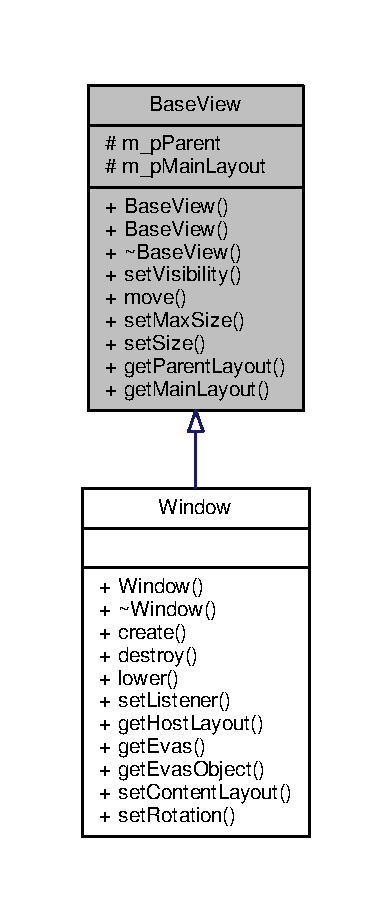
\includegraphics[width=188pt]{class_base_view__inherit__graph}
\end{center}
\end{figure}


Collaboration diagram for Base\-View\-:
\nopagebreak
\begin{figure}[H]
\begin{center}
\leavevmode
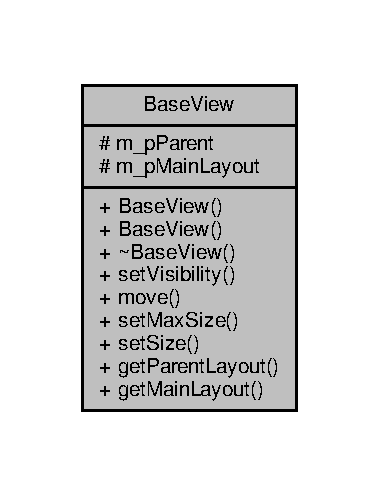
\includegraphics[width=182pt]{class_base_view__coll__graph}
\end{center}
\end{figure}
\subsection*{Public Member Functions}
\begin{DoxyCompactItemize}
\item 
\hyperlink{class_base_view_a0ea730b39012b33298fd37fa1d2c28b4}{Base\-View} (\hyperlink{class_base_view}{Base\-View} \&parent)
\item 
\hyperlink{class_base_view_ad88b86000a86a321ec237fc11eb21f00}{Base\-View} (Evas\-\_\-\-Object $\ast$parent)
\item 
virtual \hyperlink{class_base_view_a0b87986502d132344f08be851cdb15d2}{$\sim$\-Base\-View} ()
\item 
virtual void \hyperlink{class_base_view_a3fb4396cd7133b73f113251c3828538a}{set\-Visibility} (bool val)
\item 
virtual void \hyperlink{class_base_view_afa1b6656ef2b8eff83dd476e8b1e1200}{move} (int x, int y)
\item 
virtual void \hyperlink{class_base_view_a4737f13d8c9c17ecd2748e46e9f075b0}{set\-Max\-Size} (int width, int height)
\item 
virtual void \hyperlink{class_base_view_a41a081c844838223e991bfe2d1220090}{set\-Size} (int width, int height)
\item 
virtual Evas\-\_\-\-Object $\ast$ \hyperlink{class_base_view_a11e9825ed7ba6af5ad721acdbbe2762b}{get\-Parent\-Layout} () const 
\item 
virtual Evas\-\_\-\-Object $\ast$ \hyperlink{class_base_view_a4a09f445d9eb27d674382189f4ae7e14}{get\-Main\-Layout} () const 
\end{DoxyCompactItemize}
\subsection*{Protected Attributes}
\begin{DoxyCompactItemize}
\item 
Evas\-\_\-\-Object $\ast$ \hyperlink{class_base_view_af2e9d5f37dc60430d28cebcb55ffe2b4}{m\-\_\-p\-Parent}
\item 
Evas\-\_\-\-Object $\ast$ \hyperlink{class_base_view_a27bf1606488064c17a4fad81b0feb61f}{m\-\_\-p\-Main\-Layout}
\end{DoxyCompactItemize}


\subsection{Detailed Description}


Definition at line 27 of file Base\-View.\-h.



\subsection{Constructor \& Destructor Documentation}
\hypertarget{class_base_view_a0ea730b39012b33298fd37fa1d2c28b4}{\index{Base\-View@{Base\-View}!Base\-View@{Base\-View}}
\index{Base\-View@{Base\-View}!BaseView@{Base\-View}}
\subsubsection[{Base\-View}]{\setlength{\rightskip}{0pt plus 5cm}Base\-View\-::\-Base\-View (
\begin{DoxyParamCaption}
\item[{{\bf Base\-View} \&}]{parent}
\end{DoxyParamCaption}
)}}\label{class_base_view_a0ea730b39012b33298fd37fa1d2c28b4}
Constructor 
\begin{DoxyParams}{Parameters}
{\em ref.} & to parent parent view \\
\hline
\end{DoxyParams}


Definition at line 24 of file Base\-View.\-cpp.

\hypertarget{class_base_view_ad88b86000a86a321ec237fc11eb21f00}{\index{Base\-View@{Base\-View}!Base\-View@{Base\-View}}
\index{Base\-View@{Base\-View}!BaseView@{Base\-View}}
\subsubsection[{Base\-View}]{\setlength{\rightskip}{0pt plus 5cm}Base\-View\-::\-Base\-View (
\begin{DoxyParamCaption}
\item[{Evas\-\_\-\-Object $\ast$}]{parent}
\end{DoxyParamCaption}
)}}\label{class_base_view_ad88b86000a86a321ec237fc11eb21f00}
Constructor 
\begin{DoxyParams}{Parameters}
{\em pointer} & to parent Evas\-\_\-\-Object \\
\hline
\end{DoxyParams}


Definition at line 31 of file Base\-View.\-cpp.

\hypertarget{class_base_view_a0b87986502d132344f08be851cdb15d2}{\index{Base\-View@{Base\-View}!$\sim$\-Base\-View@{$\sim$\-Base\-View}}
\index{$\sim$\-Base\-View@{$\sim$\-Base\-View}!BaseView@{Base\-View}}
\subsubsection[{$\sim$\-Base\-View}]{\setlength{\rightskip}{0pt plus 5cm}Base\-View\-::$\sim$\-Base\-View (
\begin{DoxyParamCaption}
{}
\end{DoxyParamCaption}
)\hspace{0.3cm}{\ttfamily [virtual]}}}\label{class_base_view_a0b87986502d132344f08be851cdb15d2}
Destructor 

Definition at line 38 of file Base\-View.\-cpp.



\subsection{Member Function Documentation}
\hypertarget{class_base_view_a4a09f445d9eb27d674382189f4ae7e14}{\index{Base\-View@{Base\-View}!get\-Main\-Layout@{get\-Main\-Layout}}
\index{get\-Main\-Layout@{get\-Main\-Layout}!BaseView@{Base\-View}}
\subsubsection[{get\-Main\-Layout}]{\setlength{\rightskip}{0pt plus 5cm}Evas\-\_\-\-Object $\ast$ Base\-View\-::get\-Main\-Layout (
\begin{DoxyParamCaption}
{}
\end{DoxyParamCaption}
) const\hspace{0.3cm}{\ttfamily [virtual]}}}\label{class_base_view_a4a09f445d9eb27d674382189f4ae7e14}
Get main layout of view \begin{DoxyReturn}{Returns}
pointer to layout 
\end{DoxyReturn}


Definition at line 59 of file Base\-View.\-cpp.

\hypertarget{class_base_view_a11e9825ed7ba6af5ad721acdbbe2762b}{\index{Base\-View@{Base\-View}!get\-Parent\-Layout@{get\-Parent\-Layout}}
\index{get\-Parent\-Layout@{get\-Parent\-Layout}!BaseView@{Base\-View}}
\subsubsection[{get\-Parent\-Layout}]{\setlength{\rightskip}{0pt plus 5cm}Evas\-\_\-\-Object $\ast$ Base\-View\-::get\-Parent\-Layout (
\begin{DoxyParamCaption}
{}
\end{DoxyParamCaption}
) const\hspace{0.3cm}{\ttfamily [virtual]}}}\label{class_base_view_a11e9825ed7ba6af5ad721acdbbe2762b}
Get parent layout \begin{DoxyReturn}{Returns}
pointer to layout 
\end{DoxyReturn}


Definition at line 54 of file Base\-View.\-cpp.

\hypertarget{class_base_view_afa1b6656ef2b8eff83dd476e8b1e1200}{\index{Base\-View@{Base\-View}!move@{move}}
\index{move@{move}!BaseView@{Base\-View}}
\subsubsection[{move}]{\setlength{\rightskip}{0pt plus 5cm}void Base\-View\-::move (
\begin{DoxyParamCaption}
\item[{int}]{x, }
\item[{int}]{y}
\end{DoxyParamCaption}
)\hspace{0.3cm}{\ttfamily [virtual]}}}\label{class_base_view_afa1b6656ef2b8eff83dd476e8b1e1200}
Move view 
\begin{DoxyParams}{Parameters}
{\em x} & position to move the object to, in canvas. \\
\hline
{\em y} & position to move the object to, in canvas. \\
\hline
\end{DoxyParams}


Definition at line 64 of file Base\-View.\-cpp.

\hypertarget{class_base_view_a4737f13d8c9c17ecd2748e46e9f075b0}{\index{Base\-View@{Base\-View}!set\-Max\-Size@{set\-Max\-Size}}
\index{set\-Max\-Size@{set\-Max\-Size}!BaseView@{Base\-View}}
\subsubsection[{set\-Max\-Size}]{\setlength{\rightskip}{0pt plus 5cm}void Base\-View\-::set\-Max\-Size (
\begin{DoxyParamCaption}
\item[{int}]{width, }
\item[{int}]{height}
\end{DoxyParamCaption}
)\hspace{0.3cm}{\ttfamily [virtual]}}}\label{class_base_view_a4737f13d8c9c17ecd2748e46e9f075b0}
Set max size of view 
\begin{DoxyParams}{Parameters}
{\em width} & max width \\
\hline
{\em height} & max height \\
\hline
\end{DoxyParams}


Definition at line 70 of file Base\-View.\-cpp.



Here is the caller graph for this function\-:\nopagebreak
\begin{figure}[H]
\begin{center}
\leavevmode
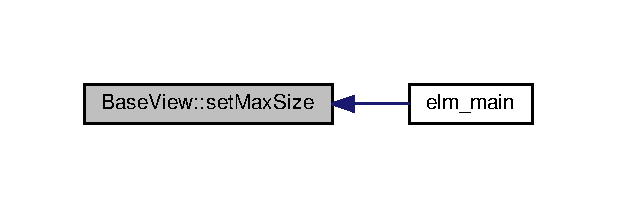
\includegraphics[width=296pt]{class_base_view_a4737f13d8c9c17ecd2748e46e9f075b0_icgraph}
\end{center}
\end{figure}


\hypertarget{class_base_view_a41a081c844838223e991bfe2d1220090}{\index{Base\-View@{Base\-View}!set\-Size@{set\-Size}}
\index{set\-Size@{set\-Size}!BaseView@{Base\-View}}
\subsubsection[{set\-Size}]{\setlength{\rightskip}{0pt plus 5cm}void Base\-View\-::set\-Size (
\begin{DoxyParamCaption}
\item[{int}]{width, }
\item[{int}]{height}
\end{DoxyParamCaption}
)\hspace{0.3cm}{\ttfamily [virtual]}}}\label{class_base_view_a41a081c844838223e991bfe2d1220090}
Set size 
\begin{DoxyParams}{Parameters}
{\em width} & width of view \\
\hline
{\em height} & height of view \\
\hline
\end{DoxyParams}


Definition at line 76 of file Base\-View.\-cpp.

\hypertarget{class_base_view_a3fb4396cd7133b73f113251c3828538a}{\index{Base\-View@{Base\-View}!set\-Visibility@{set\-Visibility}}
\index{set\-Visibility@{set\-Visibility}!BaseView@{Base\-View}}
\subsubsection[{set\-Visibility}]{\setlength{\rightskip}{0pt plus 5cm}void Base\-View\-::set\-Visibility (
\begin{DoxyParamCaption}
\item[{bool}]{val}
\end{DoxyParamCaption}
)\hspace{0.3cm}{\ttfamily [virtual]}}}\label{class_base_view_a3fb4396cd7133b73f113251c3828538a}
Set visibility 
\begin{DoxyParams}{Parameters}
{\em val} & true -\/ show, false -\/ hide \\
\hline
\end{DoxyParams}


Definition at line 43 of file Base\-View.\-cpp.



\subsection{Member Data Documentation}
\hypertarget{class_base_view_a27bf1606488064c17a4fad81b0feb61f}{\index{Base\-View@{Base\-View}!m\-\_\-p\-Main\-Layout@{m\-\_\-p\-Main\-Layout}}
\index{m\-\_\-p\-Main\-Layout@{m\-\_\-p\-Main\-Layout}!BaseView@{Base\-View}}
\subsubsection[{m\-\_\-p\-Main\-Layout}]{\setlength{\rightskip}{0pt plus 5cm}Evas\-\_\-\-Object$\ast$ Base\-View\-::m\-\_\-p\-Main\-Layout\hspace{0.3cm}{\ttfamily [protected]}}}\label{class_base_view_a27bf1606488064c17a4fad81b0feb61f}


Definition at line 88 of file Base\-View.\-h.

\hypertarget{class_base_view_af2e9d5f37dc60430d28cebcb55ffe2b4}{\index{Base\-View@{Base\-View}!m\-\_\-p\-Parent@{m\-\_\-p\-Parent}}
\index{m\-\_\-p\-Parent@{m\-\_\-p\-Parent}!BaseView@{Base\-View}}
\subsubsection[{m\-\_\-p\-Parent}]{\setlength{\rightskip}{0pt plus 5cm}Evas\-\_\-\-Object$\ast$ Base\-View\-::m\-\_\-p\-Parent\hspace{0.3cm}{\ttfamily [protected]}}}\label{class_base_view_af2e9d5f37dc60430d28cebcb55ffe2b4}


Definition at line 87 of file Base\-View.\-h.



The documentation for this class was generated from the following files\-:\begin{DoxyCompactItemize}
\item 
\hyperlink{_base_view_8h}{Base\-View.\-h}\item 
\hyperlink{_base_view_8cpp}{Base\-View.\-cpp}\end{DoxyCompactItemize}

\hypertarget{class_drawing_content}{\section{Drawing\-Content Class Reference}
\label{class_drawing_content}\index{Drawing\-Content@{Drawing\-Content}}
}


{\ttfamily \#include $<$Drawing\-Content.\-h$>$}



Inheritance diagram for Drawing\-Content\-:\nopagebreak
\begin{figure}[H]
\begin{center}
\leavevmode
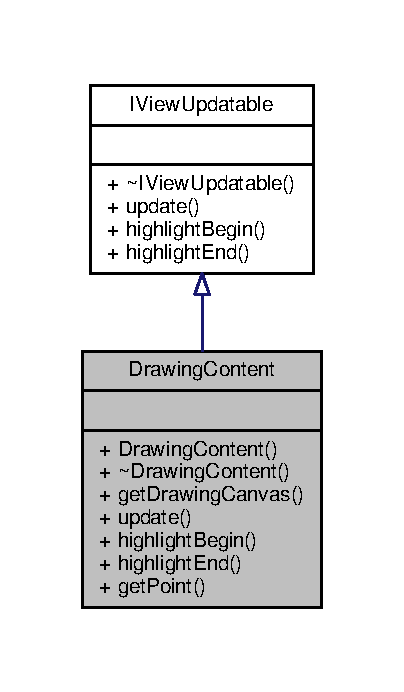
\includegraphics[width=194pt]{class_drawing_content__inherit__graph}
\end{center}
\end{figure}


Collaboration diagram for Drawing\-Content\-:
\nopagebreak
\begin{figure}[H]
\begin{center}
\leavevmode
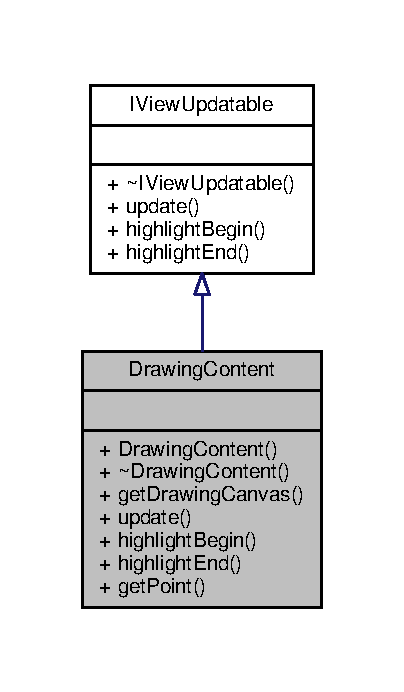
\includegraphics[width=194pt]{class_drawing_content__coll__graph}
\end{center}
\end{figure}
\subsection*{Public Member Functions}
\begin{DoxyCompactItemize}
\item 
\hyperlink{class_drawing_content_a7d8a1eb05da8003a6f849a59f6d52728}{Drawing\-Content} (Evas\-\_\-\-Object $\ast$main\-Layout)
\item 
virtual \hyperlink{class_drawing_content_aaccb2eb2a8202975bd7e03152f0b7eb4}{$\sim$\-Drawing\-Content} ()
\item 
Evas\-\_\-\-Object $\ast$ \hyperlink{class_drawing_content_ade92d7e68527c0df61b085d1808ee182}{get\-Drawing\-Canvas} ()
\item 
void \hyperlink{class_drawing_content_ae162f5d085ebdb6bd1d13bd2c895495a}{update} ()
\item 
void \hyperlink{class_drawing_content_a9c9c2b7812ac5ec2cff9d9712606c8fa}{highlight\-Begin} (\hyperlink{class_point}{Point} \&point)
\item 
void \hyperlink{class_drawing_content_aef196b253d9057b2396d7aa0e6aa5646}{highlight\-End} ()
\item 
bool \hyperlink{class_drawing_content_a991ef6e99883102af69b1af56b662be8}{get\-Point} (int x, int y, Graphic\-Point \&graphic\-Point)
\end{DoxyCompactItemize}


\subsection{Detailed Description}


Definition at line 18 of file Drawing\-Content.\-h.



\subsection{Constructor \& Destructor Documentation}
\hypertarget{class_drawing_content_a7d8a1eb05da8003a6f849a59f6d52728}{\index{Drawing\-Content@{Drawing\-Content}!Drawing\-Content@{Drawing\-Content}}
\index{Drawing\-Content@{Drawing\-Content}!DrawingContent@{Drawing\-Content}}
\subsubsection[{Drawing\-Content}]{\setlength{\rightskip}{0pt plus 5cm}Drawing\-Content\-::\-Drawing\-Content (
\begin{DoxyParamCaption}
\item[{Evas\-\_\-\-Object $\ast$}]{main\-Layout}
\end{DoxyParamCaption}
)}}\label{class_drawing_content_a7d8a1eb05da8003a6f849a59f6d52728}


Definition at line 19 of file Drawing\-Content.\-cpp.

\hypertarget{class_drawing_content_aaccb2eb2a8202975bd7e03152f0b7eb4}{\index{Drawing\-Content@{Drawing\-Content}!$\sim$\-Drawing\-Content@{$\sim$\-Drawing\-Content}}
\index{$\sim$\-Drawing\-Content@{$\sim$\-Drawing\-Content}!DrawingContent@{Drawing\-Content}}
\subsubsection[{$\sim$\-Drawing\-Content}]{\setlength{\rightskip}{0pt plus 5cm}Drawing\-Content\-::$\sim$\-Drawing\-Content (
\begin{DoxyParamCaption}
{}
\end{DoxyParamCaption}
)\hspace{0.3cm}{\ttfamily [virtual]}}}\label{class_drawing_content_aaccb2eb2a8202975bd7e03152f0b7eb4}


Definition at line 25 of file Drawing\-Content.\-cpp.



\subsection{Member Function Documentation}
\hypertarget{class_drawing_content_ade92d7e68527c0df61b085d1808ee182}{\index{Drawing\-Content@{Drawing\-Content}!get\-Drawing\-Canvas@{get\-Drawing\-Canvas}}
\index{get\-Drawing\-Canvas@{get\-Drawing\-Canvas}!DrawingContent@{Drawing\-Content}}
\subsubsection[{get\-Drawing\-Canvas}]{\setlength{\rightskip}{0pt plus 5cm}Evas\-\_\-\-Object $\ast$ Drawing\-Content\-::get\-Drawing\-Canvas (
\begin{DoxyParamCaption}
{}
\end{DoxyParamCaption}
)}}\label{class_drawing_content_ade92d7e68527c0df61b085d1808ee182}


Definition at line 56 of file Drawing\-Content.\-cpp.

\hypertarget{class_drawing_content_a991ef6e99883102af69b1af56b662be8}{\index{Drawing\-Content@{Drawing\-Content}!get\-Point@{get\-Point}}
\index{get\-Point@{get\-Point}!DrawingContent@{Drawing\-Content}}
\subsubsection[{get\-Point}]{\setlength{\rightskip}{0pt plus 5cm}bool Drawing\-Content\-::get\-Point (
\begin{DoxyParamCaption}
\item[{int}]{x, }
\item[{int}]{y, }
\item[{Graphic\-Point \&}]{graphic\-Point}
\end{DoxyParamCaption}
)}}\label{class_drawing_content_a991ef6e99883102af69b1af56b662be8}


Definition at line 141 of file Drawing\-Content.\-cpp.

\hypertarget{class_drawing_content_a9c9c2b7812ac5ec2cff9d9712606c8fa}{\index{Drawing\-Content@{Drawing\-Content}!highlight\-Begin@{highlight\-Begin}}
\index{highlight\-Begin@{highlight\-Begin}!DrawingContent@{Drawing\-Content}}
\subsubsection[{highlight\-Begin}]{\setlength{\rightskip}{0pt plus 5cm}void Drawing\-Content\-::highlight\-Begin (
\begin{DoxyParamCaption}
\item[{{\bf Point} \&}]{point}
\end{DoxyParamCaption}
)\hspace{0.3cm}{\ttfamily [virtual]}}}\label{class_drawing_content_a9c9c2b7812ac5ec2cff9d9712606c8fa}


Implements \hyperlink{class_i_view_updatable_aaf59f7e755222be617f6d24da32b7c47}{I\-View\-Updatable}.



Definition at line 70 of file Drawing\-Content.\-cpp.



Here is the call graph for this function\-:\nopagebreak
\begin{figure}[H]
\begin{center}
\leavevmode
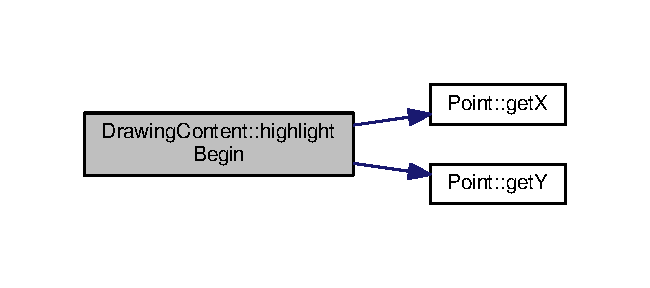
\includegraphics[width=312pt]{class_drawing_content_a9c9c2b7812ac5ec2cff9d9712606c8fa_cgraph}
\end{center}
\end{figure}


\hypertarget{class_drawing_content_aef196b253d9057b2396d7aa0e6aa5646}{\index{Drawing\-Content@{Drawing\-Content}!highlight\-End@{highlight\-End}}
\index{highlight\-End@{highlight\-End}!DrawingContent@{Drawing\-Content}}
\subsubsection[{highlight\-End}]{\setlength{\rightskip}{0pt plus 5cm}void Drawing\-Content\-::highlight\-End (
\begin{DoxyParamCaption}
{}
\end{DoxyParamCaption}
)\hspace{0.3cm}{\ttfamily [virtual]}}}\label{class_drawing_content_aef196b253d9057b2396d7aa0e6aa5646}


Implements \hyperlink{class_i_view_updatable_a3c3f25cec4eb59d005aa229b60dc0bdf}{I\-View\-Updatable}.



Definition at line 82 of file Drawing\-Content.\-cpp.

\hypertarget{class_drawing_content_ae162f5d085ebdb6bd1d13bd2c895495a}{\index{Drawing\-Content@{Drawing\-Content}!update@{update}}
\index{update@{update}!DrawingContent@{Drawing\-Content}}
\subsubsection[{update}]{\setlength{\rightskip}{0pt plus 5cm}void Drawing\-Content\-::update (
\begin{DoxyParamCaption}
{}
\end{DoxyParamCaption}
)\hspace{0.3cm}{\ttfamily [virtual]}}}\label{class_drawing_content_ae162f5d085ebdb6bd1d13bd2c895495a}


Implements \hyperlink{class_i_view_updatable_a7bb2c3735909fe059e5030ad3dde42ff}{I\-View\-Updatable}.



Definition at line 61 of file Drawing\-Content.\-cpp.



The documentation for this class was generated from the following files\-:\begin{DoxyCompactItemize}
\item 
\hyperlink{_drawing_content_8h}{Drawing\-Content.\-h}\item 
\hyperlink{_drawing_content_8cpp}{Drawing\-Content.\-cpp}\end{DoxyCompactItemize}

\hypertarget{class_geometry_object_factory}{\section{Geometry\-Object\-Factory Class Reference}
\label{class_geometry_object_factory}\index{Geometry\-Object\-Factory@{Geometry\-Object\-Factory}}
}


{\ttfamily \#include $<$Geometry\-Object\-Factory.\-h$>$}



Collaboration diagram for Geometry\-Object\-Factory\-:
\nopagebreak
\begin{figure}[H]
\begin{center}
\leavevmode
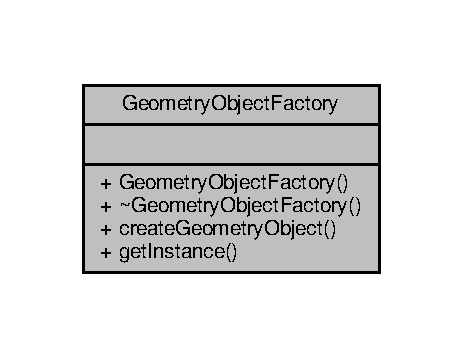
\includegraphics[width=222pt]{class_geometry_object_factory__coll__graph}
\end{center}
\end{figure}
\subsection*{Public Member Functions}
\begin{DoxyCompactItemize}
\item 
\hyperlink{class_geometry_object_factory_a759b281e3db965d1517d1490ef6d715d}{Geometry\-Object\-Factory} ()
\item 
virtual \hyperlink{class_geometry_object_factory_a1cc18355ea7a691ac628dcbc0b8cc76d}{$\sim$\-Geometry\-Object\-Factory} ()
\item 
\hyperlink{class_i_geometry_object}{I\-Geometry\-Object} $\ast$ \hyperlink{class_geometry_object_factory_ac1b7a6573f7dee62d37ff55e23ea16bc}{create\-Geometry\-Object} (\hyperlink{_geometry_objects_types_8h_adea8b8c3a289ca1fc1450d9424dcd33d}{Geometry\-Objects\-Types} type)
\end{DoxyCompactItemize}
\subsection*{Static Public Member Functions}
\begin{DoxyCompactItemize}
\item 
static \hyperlink{class_geometry_object_factory}{Geometry\-Object\-Factory} \& \hyperlink{class_geometry_object_factory_a517fdd10bb45b6d7cf924d9cbacca6d1}{get\-Instance} ()
\end{DoxyCompactItemize}


\subsection{Detailed Description}


Definition at line 14 of file Geometry\-Object\-Factory.\-h.



\subsection{Constructor \& Destructor Documentation}
\hypertarget{class_geometry_object_factory_a759b281e3db965d1517d1490ef6d715d}{\index{Geometry\-Object\-Factory@{Geometry\-Object\-Factory}!Geometry\-Object\-Factory@{Geometry\-Object\-Factory}}
\index{Geometry\-Object\-Factory@{Geometry\-Object\-Factory}!GeometryObjectFactory@{Geometry\-Object\-Factory}}
\subsubsection[{Geometry\-Object\-Factory}]{\setlength{\rightskip}{0pt plus 5cm}Geometry\-Object\-Factory\-::\-Geometry\-Object\-Factory (
\begin{DoxyParamCaption}
{}
\end{DoxyParamCaption}
)}}\label{class_geometry_object_factory_a759b281e3db965d1517d1490ef6d715d}


Definition at line 12 of file Geometry\-Object\-Factory.\-cpp.

\hypertarget{class_geometry_object_factory_a1cc18355ea7a691ac628dcbc0b8cc76d}{\index{Geometry\-Object\-Factory@{Geometry\-Object\-Factory}!$\sim$\-Geometry\-Object\-Factory@{$\sim$\-Geometry\-Object\-Factory}}
\index{$\sim$\-Geometry\-Object\-Factory@{$\sim$\-Geometry\-Object\-Factory}!GeometryObjectFactory@{Geometry\-Object\-Factory}}
\subsubsection[{$\sim$\-Geometry\-Object\-Factory}]{\setlength{\rightskip}{0pt plus 5cm}Geometry\-Object\-Factory\-::$\sim$\-Geometry\-Object\-Factory (
\begin{DoxyParamCaption}
{}
\end{DoxyParamCaption}
)\hspace{0.3cm}{\ttfamily [virtual]}}}\label{class_geometry_object_factory_a1cc18355ea7a691ac628dcbc0b8cc76d}


Definition at line 17 of file Geometry\-Object\-Factory.\-cpp.



\subsection{Member Function Documentation}
\hypertarget{class_geometry_object_factory_ac1b7a6573f7dee62d37ff55e23ea16bc}{\index{Geometry\-Object\-Factory@{Geometry\-Object\-Factory}!create\-Geometry\-Object@{create\-Geometry\-Object}}
\index{create\-Geometry\-Object@{create\-Geometry\-Object}!GeometryObjectFactory@{Geometry\-Object\-Factory}}
\subsubsection[{create\-Geometry\-Object}]{\setlength{\rightskip}{0pt plus 5cm}{\bf I\-Geometry\-Object} $\ast$ Geometry\-Object\-Factory\-::create\-Geometry\-Object (
\begin{DoxyParamCaption}
\item[{{\bf Geometry\-Objects\-Types}}]{type}
\end{DoxyParamCaption}
)}}\label{class_geometry_object_factory_ac1b7a6573f7dee62d37ff55e23ea16bc}


Definition at line 21 of file Geometry\-Object\-Factory.\-cpp.

\hypertarget{class_geometry_object_factory_a517fdd10bb45b6d7cf924d9cbacca6d1}{\index{Geometry\-Object\-Factory@{Geometry\-Object\-Factory}!get\-Instance@{get\-Instance}}
\index{get\-Instance@{get\-Instance}!GeometryObjectFactory@{Geometry\-Object\-Factory}}
\subsubsection[{get\-Instance}]{\setlength{\rightskip}{0pt plus 5cm}{\bf Geometry\-Object\-Factory} \& Geometry\-Object\-Factory\-::get\-Instance (
\begin{DoxyParamCaption}
{}
\end{DoxyParamCaption}
)\hspace{0.3cm}{\ttfamily [static]}}}\label{class_geometry_object_factory_a517fdd10bb45b6d7cf924d9cbacca6d1}


Definition at line 36 of file Geometry\-Object\-Factory.\-cpp.



Here is the caller graph for this function\-:\nopagebreak
\begin{figure}[H]
\begin{center}
\leavevmode
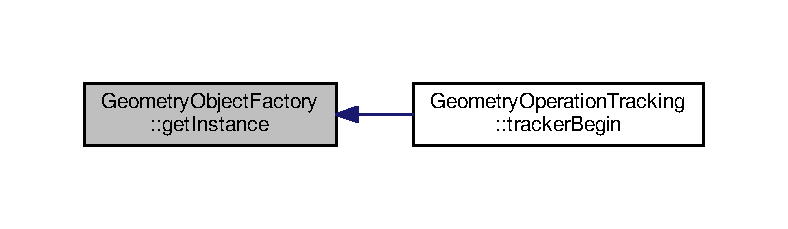
\includegraphics[width=350pt]{class_geometry_object_factory_a517fdd10bb45b6d7cf924d9cbacca6d1_icgraph}
\end{center}
\end{figure}




The documentation for this class was generated from the following files\-:\begin{DoxyCompactItemize}
\item 
\hyperlink{_geometry_object_factory_8h}{Geometry\-Object\-Factory.\-h}\item 
\hyperlink{_geometry_object_factory_8cpp}{Geometry\-Object\-Factory.\-cpp}\end{DoxyCompactItemize}

\hypertarget{class_geometry_objects_manager}{\section{Geometry\-Objects\-Manager Class Reference}
\label{class_geometry_objects_manager}\index{Geometry\-Objects\-Manager@{Geometry\-Objects\-Manager}}
}


{\ttfamily \#include $<$Geometry\-Objects\-Manager.\-h$>$}



Collaboration diagram for Geometry\-Objects\-Manager\-:
\nopagebreak
\begin{figure}[H]
\begin{center}
\leavevmode
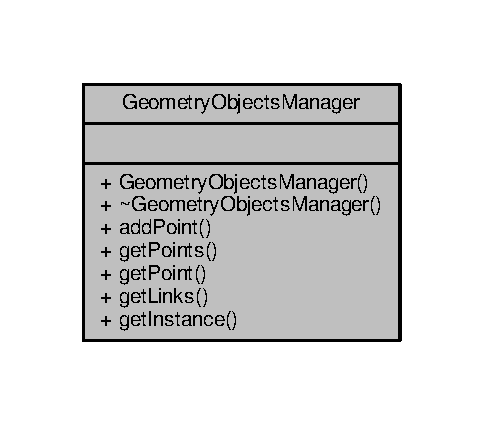
\includegraphics[width=232pt]{class_geometry_objects_manager__coll__graph}
\end{center}
\end{figure}
\subsection*{Public Member Functions}
\begin{DoxyCompactItemize}
\item 
\hyperlink{class_geometry_objects_manager_ac1847098c6290faaef1f64b1bb9f7163}{Geometry\-Objects\-Manager} ()
\item 
virtual \hyperlink{class_geometry_objects_manager_a4fe85a06b6810491f953b0463692e8e8}{$\sim$\-Geometry\-Objects\-Manager} ()
\item 
void \hyperlink{class_geometry_objects_manager_ab929b8e262f10bc34cf8f296794f19c2}{add\-Point} (\hyperlink{class_point}{Point} \&point)
\item 
void \hyperlink{class_geometry_objects_manager_a7023c883729a9301d4e11a3bce43f8dd}{get\-Points} (vector$<$ \hyperlink{class_point}{Point} $>$ \&points)
\item 
bool \hyperlink{class_geometry_objects_manager_a4c9b1d61333a56175336d6d12f9e0b0c}{get\-Point} (int x, int y, \hyperlink{class_point}{Point} \&point)
\item 
void \hyperlink{class_geometry_objects_manager_af6ec7cbc6947a1fe9d32861cefb3515e}{get\-Links} (vector$<$ \hyperlink{class_points_link}{Points\-Link} $>$ \&links)
\end{DoxyCompactItemize}
\subsection*{Static Public Member Functions}
\begin{DoxyCompactItemize}
\item 
static \hyperlink{class_geometry_objects_manager}{Geometry\-Objects\-Manager} \& \hyperlink{class_geometry_objects_manager_a34e70b86d34d51108132414cd0a57ab8}{get\-Instance} ()
\end{DoxyCompactItemize}


\subsection{Detailed Description}


Definition at line 17 of file Geometry\-Objects\-Manager.\-h.



\subsection{Constructor \& Destructor Documentation}
\hypertarget{class_geometry_objects_manager_ac1847098c6290faaef1f64b1bb9f7163}{\index{Geometry\-Objects\-Manager@{Geometry\-Objects\-Manager}!Geometry\-Objects\-Manager@{Geometry\-Objects\-Manager}}
\index{Geometry\-Objects\-Manager@{Geometry\-Objects\-Manager}!GeometryObjectsManager@{Geometry\-Objects\-Manager}}
\subsubsection[{Geometry\-Objects\-Manager}]{\setlength{\rightskip}{0pt plus 5cm}Geometry\-Objects\-Manager\-::\-Geometry\-Objects\-Manager (
\begin{DoxyParamCaption}
{}
\end{DoxyParamCaption}
)}}\label{class_geometry_objects_manager_ac1847098c6290faaef1f64b1bb9f7163}


Definition at line 12 of file Geometry\-Objects\-Manager.\-cpp.

\hypertarget{class_geometry_objects_manager_a4fe85a06b6810491f953b0463692e8e8}{\index{Geometry\-Objects\-Manager@{Geometry\-Objects\-Manager}!$\sim$\-Geometry\-Objects\-Manager@{$\sim$\-Geometry\-Objects\-Manager}}
\index{$\sim$\-Geometry\-Objects\-Manager@{$\sim$\-Geometry\-Objects\-Manager}!GeometryObjectsManager@{Geometry\-Objects\-Manager}}
\subsubsection[{$\sim$\-Geometry\-Objects\-Manager}]{\setlength{\rightskip}{0pt plus 5cm}Geometry\-Objects\-Manager\-::$\sim$\-Geometry\-Objects\-Manager (
\begin{DoxyParamCaption}
{}
\end{DoxyParamCaption}
)\hspace{0.3cm}{\ttfamily [virtual]}}}\label{class_geometry_objects_manager_a4fe85a06b6810491f953b0463692e8e8}


Definition at line 16 of file Geometry\-Objects\-Manager.\-cpp.



\subsection{Member Function Documentation}
\hypertarget{class_geometry_objects_manager_ab929b8e262f10bc34cf8f296794f19c2}{\index{Geometry\-Objects\-Manager@{Geometry\-Objects\-Manager}!add\-Point@{add\-Point}}
\index{add\-Point@{add\-Point}!GeometryObjectsManager@{Geometry\-Objects\-Manager}}
\subsubsection[{add\-Point}]{\setlength{\rightskip}{0pt plus 5cm}void Geometry\-Objects\-Manager\-::add\-Point (
\begin{DoxyParamCaption}
\item[{{\bf Point} \&}]{point}
\end{DoxyParamCaption}
)}}\label{class_geometry_objects_manager_ab929b8e262f10bc34cf8f296794f19c2}


Definition at line 20 of file Geometry\-Objects\-Manager.\-cpp.



Here is the caller graph for this function\-:\nopagebreak
\begin{figure}[H]
\begin{center}
\leavevmode
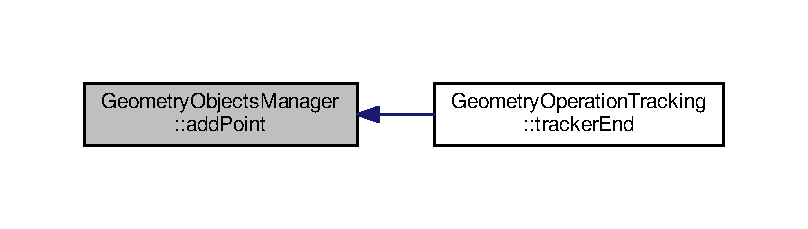
\includegraphics[width=350pt]{class_geometry_objects_manager_ab929b8e262f10bc34cf8f296794f19c2_icgraph}
\end{center}
\end{figure}


\hypertarget{class_geometry_objects_manager_a34e70b86d34d51108132414cd0a57ab8}{\index{Geometry\-Objects\-Manager@{Geometry\-Objects\-Manager}!get\-Instance@{get\-Instance}}
\index{get\-Instance@{get\-Instance}!GeometryObjectsManager@{Geometry\-Objects\-Manager}}
\subsubsection[{get\-Instance}]{\setlength{\rightskip}{0pt plus 5cm}{\bf Geometry\-Objects\-Manager} \& Geometry\-Objects\-Manager\-::get\-Instance (
\begin{DoxyParamCaption}
{}
\end{DoxyParamCaption}
)\hspace{0.3cm}{\ttfamily [static]}}}\label{class_geometry_objects_manager_a34e70b86d34d51108132414cd0a57ab8}


Definition at line 51 of file Geometry\-Objects\-Manager.\-cpp.



Here is the caller graph for this function\-:\nopagebreak
\begin{figure}[H]
\begin{center}
\leavevmode
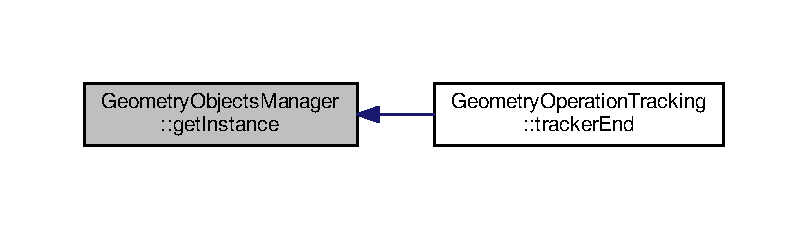
\includegraphics[width=350pt]{class_geometry_objects_manager_a34e70b86d34d51108132414cd0a57ab8_icgraph}
\end{center}
\end{figure}


\hypertarget{class_geometry_objects_manager_af6ec7cbc6947a1fe9d32861cefb3515e}{\index{Geometry\-Objects\-Manager@{Geometry\-Objects\-Manager}!get\-Links@{get\-Links}}
\index{get\-Links@{get\-Links}!GeometryObjectsManager@{Geometry\-Objects\-Manager}}
\subsubsection[{get\-Links}]{\setlength{\rightskip}{0pt plus 5cm}void Geometry\-Objects\-Manager\-::get\-Links (
\begin{DoxyParamCaption}
\item[{vector$<$ {\bf Points\-Link} $>$ \&}]{links}
\end{DoxyParamCaption}
)}}\label{class_geometry_objects_manager_af6ec7cbc6947a1fe9d32861cefb3515e}
\hypertarget{class_geometry_objects_manager_a4c9b1d61333a56175336d6d12f9e0b0c}{\index{Geometry\-Objects\-Manager@{Geometry\-Objects\-Manager}!get\-Point@{get\-Point}}
\index{get\-Point@{get\-Point}!GeometryObjectsManager@{Geometry\-Objects\-Manager}}
\subsubsection[{get\-Point}]{\setlength{\rightskip}{0pt plus 5cm}bool Geometry\-Objects\-Manager\-::get\-Point (
\begin{DoxyParamCaption}
\item[{int}]{x, }
\item[{int}]{y, }
\item[{{\bf Point} \&}]{point}
\end{DoxyParamCaption}
)}}\label{class_geometry_objects_manager_a4c9b1d61333a56175336d6d12f9e0b0c}


Definition at line 30 of file Geometry\-Objects\-Manager.\-cpp.

\hypertarget{class_geometry_objects_manager_a7023c883729a9301d4e11a3bce43f8dd}{\index{Geometry\-Objects\-Manager@{Geometry\-Objects\-Manager}!get\-Points@{get\-Points}}
\index{get\-Points@{get\-Points}!GeometryObjectsManager@{Geometry\-Objects\-Manager}}
\subsubsection[{get\-Points}]{\setlength{\rightskip}{0pt plus 5cm}void Geometry\-Objects\-Manager\-::get\-Points (
\begin{DoxyParamCaption}
\item[{vector$<$ {\bf Point} $>$ \&}]{points}
\end{DoxyParamCaption}
)}}\label{class_geometry_objects_manager_a7023c883729a9301d4e11a3bce43f8dd}


Definition at line 25 of file Geometry\-Objects\-Manager.\-cpp.



The documentation for this class was generated from the following files\-:\begin{DoxyCompactItemize}
\item 
\hyperlink{_geometry_objects_manager_8h}{Geometry\-Objects\-Manager.\-h}\item 
\hyperlink{_geometry_objects_manager_8cpp}{Geometry\-Objects\-Manager.\-cpp}\end{DoxyCompactItemize}

\hypertarget{class_geometry_operation_tracking}{\section{Geometry\-Operation\-Tracking Class Reference}
\label{class_geometry_operation_tracking}\index{Geometry\-Operation\-Tracking@{Geometry\-Operation\-Tracking}}
}


{\ttfamily \#include $<$Geometry\-Operation\-Tracking.\-h$>$}



Inheritance diagram for Geometry\-Operation\-Tracking\-:\nopagebreak
\begin{figure}[H]
\begin{center}
\leavevmode
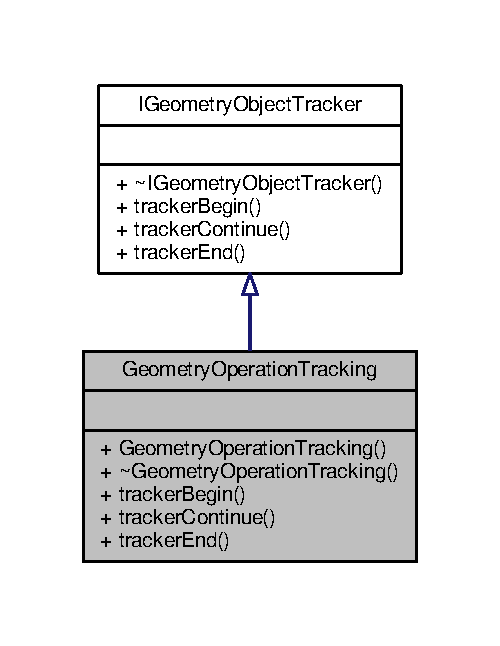
\includegraphics[width=240pt]{class_geometry_operation_tracking__inherit__graph}
\end{center}
\end{figure}


Collaboration diagram for Geometry\-Operation\-Tracking\-:
\nopagebreak
\begin{figure}[H]
\begin{center}
\leavevmode
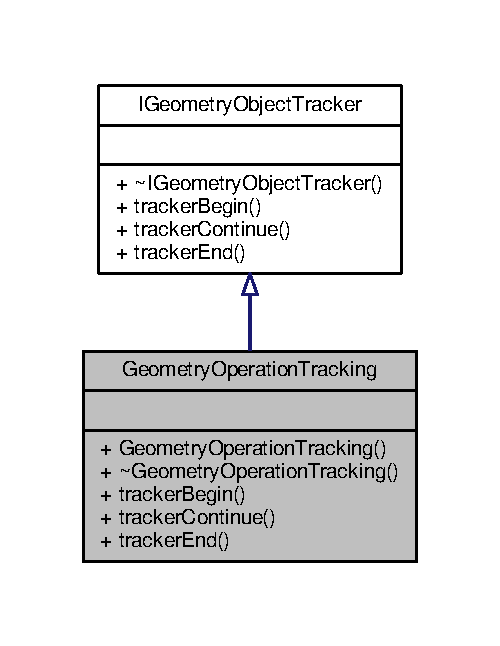
\includegraphics[width=240pt]{class_geometry_operation_tracking__coll__graph}
\end{center}
\end{figure}
\subsection*{Public Member Functions}
\begin{DoxyCompactItemize}
\item 
\hyperlink{class_geometry_operation_tracking_a527a60065b436171371c23e39ed8ebbd}{Geometry\-Operation\-Tracking} (\hyperlink{class_i_view_updatable}{I\-View\-Updatable} \&view\-Updater)
\item 
virtual \hyperlink{class_geometry_operation_tracking_a7f8681a53d38c0df0ffbbf25cb0ae0ec}{$\sim$\-Geometry\-Operation\-Tracking} ()
\item 
void \hyperlink{class_geometry_operation_tracking_a70bd6c4d97d234b40fd651ae8e64f11c}{tracker\-Begin} (int x, int y)
\item 
void \hyperlink{class_geometry_operation_tracking_acc5cf88d35759c05a5e8e7ffe24ee3d6}{tracker\-Continue} (int x, int y)
\item 
void \hyperlink{class_geometry_operation_tracking_ac67cebded53099bd604c4ffbef125080}{tracker\-End} (int x, int y)
\end{DoxyCompactItemize}


\subsection{Detailed Description}


Definition at line 19 of file Geometry\-Operation\-Tracking.\-h.



\subsection{Constructor \& Destructor Documentation}
\hypertarget{class_geometry_operation_tracking_a527a60065b436171371c23e39ed8ebbd}{\index{Geometry\-Operation\-Tracking@{Geometry\-Operation\-Tracking}!Geometry\-Operation\-Tracking@{Geometry\-Operation\-Tracking}}
\index{Geometry\-Operation\-Tracking@{Geometry\-Operation\-Tracking}!GeometryOperationTracking@{Geometry\-Operation\-Tracking}}
\subsubsection[{Geometry\-Operation\-Tracking}]{\setlength{\rightskip}{0pt plus 5cm}Geometry\-Operation\-Tracking\-::\-Geometry\-Operation\-Tracking (
\begin{DoxyParamCaption}
\item[{{\bf I\-View\-Updatable} \&}]{view\-Updater}
\end{DoxyParamCaption}
)}}\label{class_geometry_operation_tracking_a527a60065b436171371c23e39ed8ebbd}


Definition at line 12 of file Geometry\-Operation\-Tracking.\-cpp.

\hypertarget{class_geometry_operation_tracking_a7f8681a53d38c0df0ffbbf25cb0ae0ec}{\index{Geometry\-Operation\-Tracking@{Geometry\-Operation\-Tracking}!$\sim$\-Geometry\-Operation\-Tracking@{$\sim$\-Geometry\-Operation\-Tracking}}
\index{$\sim$\-Geometry\-Operation\-Tracking@{$\sim$\-Geometry\-Operation\-Tracking}!GeometryOperationTracking@{Geometry\-Operation\-Tracking}}
\subsubsection[{$\sim$\-Geometry\-Operation\-Tracking}]{\setlength{\rightskip}{0pt plus 5cm}Geometry\-Operation\-Tracking\-::$\sim$\-Geometry\-Operation\-Tracking (
\begin{DoxyParamCaption}
{}
\end{DoxyParamCaption}
)\hspace{0.3cm}{\ttfamily [virtual]}}}\label{class_geometry_operation_tracking_a7f8681a53d38c0df0ffbbf25cb0ae0ec}


Definition at line 17 of file Geometry\-Operation\-Tracking.\-cpp.



\subsection{Member Function Documentation}
\hypertarget{class_geometry_operation_tracking_a70bd6c4d97d234b40fd651ae8e64f11c}{\index{Geometry\-Operation\-Tracking@{Geometry\-Operation\-Tracking}!tracker\-Begin@{tracker\-Begin}}
\index{tracker\-Begin@{tracker\-Begin}!GeometryOperationTracking@{Geometry\-Operation\-Tracking}}
\subsubsection[{tracker\-Begin}]{\setlength{\rightskip}{0pt plus 5cm}void Geometry\-Operation\-Tracking\-::tracker\-Begin (
\begin{DoxyParamCaption}
\item[{int}]{x, }
\item[{int}]{y}
\end{DoxyParamCaption}
)\hspace{0.3cm}{\ttfamily [virtual]}}}\label{class_geometry_operation_tracking_a70bd6c4d97d234b40fd651ae8e64f11c}


Implements \hyperlink{class_i_geometry_object_tracker_a26378a17758fe170cb8187a9e604cda4}{I\-Geometry\-Object\-Tracker}.



Definition at line 22 of file Geometry\-Operation\-Tracking.\-cpp.



Here is the call graph for this function\-:\nopagebreak
\begin{figure}[H]
\begin{center}
\leavevmode
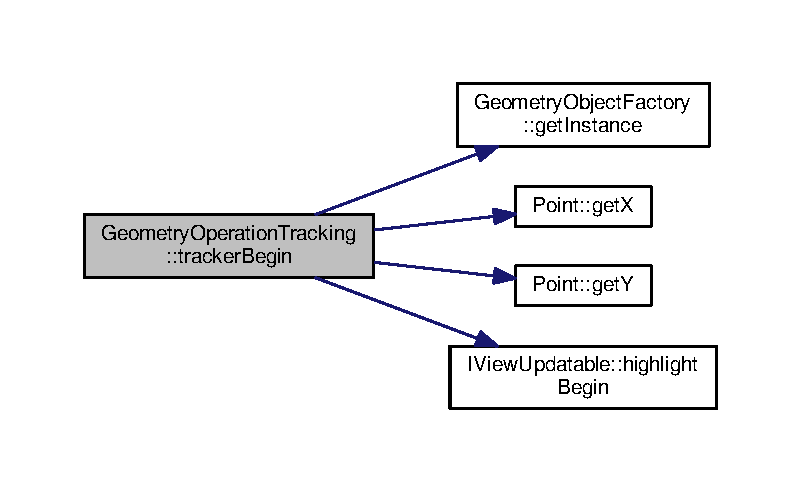
\includegraphics[width=350pt]{class_geometry_operation_tracking_a70bd6c4d97d234b40fd651ae8e64f11c_cgraph}
\end{center}
\end{figure}


\hypertarget{class_geometry_operation_tracking_acc5cf88d35759c05a5e8e7ffe24ee3d6}{\index{Geometry\-Operation\-Tracking@{Geometry\-Operation\-Tracking}!tracker\-Continue@{tracker\-Continue}}
\index{tracker\-Continue@{tracker\-Continue}!GeometryOperationTracking@{Geometry\-Operation\-Tracking}}
\subsubsection[{tracker\-Continue}]{\setlength{\rightskip}{0pt plus 5cm}void Geometry\-Operation\-Tracking\-::tracker\-Continue (
\begin{DoxyParamCaption}
\item[{int}]{x, }
\item[{int}]{y}
\end{DoxyParamCaption}
)\hspace{0.3cm}{\ttfamily [virtual]}}}\label{class_geometry_operation_tracking_acc5cf88d35759c05a5e8e7ffe24ee3d6}


Implements \hyperlink{class_i_geometry_object_tracker_a2bcfcca91ae8aa0db1553bb9459c862c}{I\-Geometry\-Object\-Tracker}.



Definition at line 45 of file Geometry\-Operation\-Tracking.\-cpp.

\hypertarget{class_geometry_operation_tracking_ac67cebded53099bd604c4ffbef125080}{\index{Geometry\-Operation\-Tracking@{Geometry\-Operation\-Tracking}!tracker\-End@{tracker\-End}}
\index{tracker\-End@{tracker\-End}!GeometryOperationTracking@{Geometry\-Operation\-Tracking}}
\subsubsection[{tracker\-End}]{\setlength{\rightskip}{0pt plus 5cm}void Geometry\-Operation\-Tracking\-::tracker\-End (
\begin{DoxyParamCaption}
\item[{int}]{x, }
\item[{int}]{y}
\end{DoxyParamCaption}
)\hspace{0.3cm}{\ttfamily [virtual]}}}\label{class_geometry_operation_tracking_ac67cebded53099bd604c4ffbef125080}


Implements \hyperlink{class_i_geometry_object_tracker_a92053b85849a8796e5ba01dba50a01fc}{I\-Geometry\-Object\-Tracker}.



Definition at line 62 of file Geometry\-Operation\-Tracking.\-cpp.



Here is the call graph for this function\-:\nopagebreak
\begin{figure}[H]
\begin{center}
\leavevmode
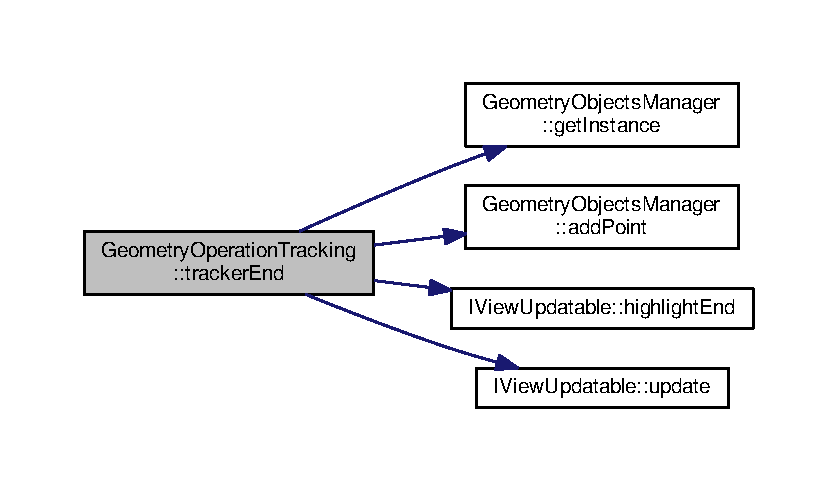
\includegraphics[width=350pt]{class_geometry_operation_tracking_ac67cebded53099bd604c4ffbef125080_cgraph}
\end{center}
\end{figure}




The documentation for this class was generated from the following files\-:\begin{DoxyCompactItemize}
\item 
\hyperlink{_geometry_operation_tracking_8h}{Geometry\-Operation\-Tracking.\-h}\item 
\hyperlink{_geometry_operation_tracking_8cpp}{Geometry\-Operation\-Tracking.\-cpp}\end{DoxyCompactItemize}

\hypertarget{class_i_geometry_object}{\section{I\-Geometry\-Object Class Reference}
\label{class_i_geometry_object}\index{I\-Geometry\-Object@{I\-Geometry\-Object}}
}


{\ttfamily \#include $<$I\-Geometry\-Object.\-h$>$}



Inheritance diagram for I\-Geometry\-Object\-:\nopagebreak
\begin{figure}[H]
\begin{center}
\leavevmode
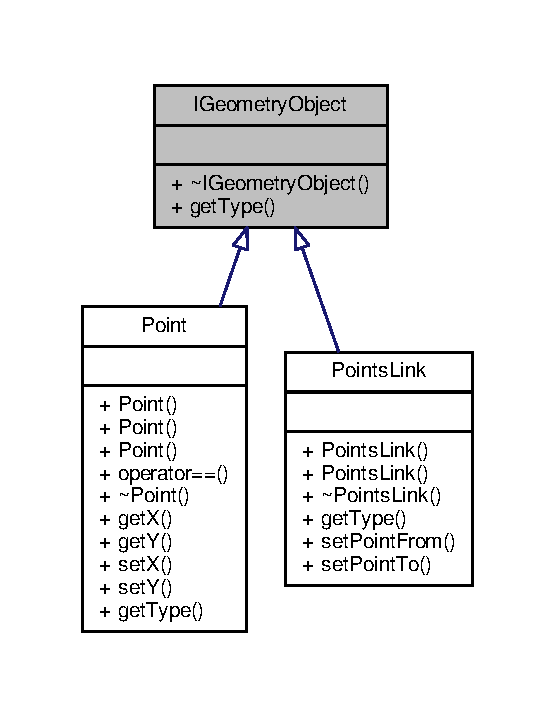
\includegraphics[width=267pt]{class_i_geometry_object__inherit__graph}
\end{center}
\end{figure}


Collaboration diagram for I\-Geometry\-Object\-:
\nopagebreak
\begin{figure}[H]
\begin{center}
\leavevmode
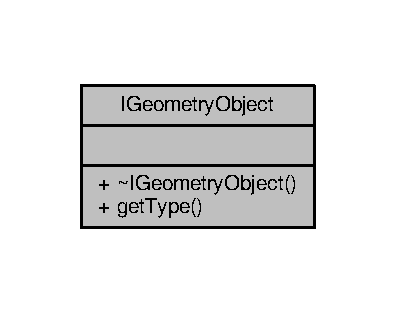
\includegraphics[width=190pt]{class_i_geometry_object__coll__graph}
\end{center}
\end{figure}
\subsection*{Public Member Functions}
\begin{DoxyCompactItemize}
\item 
virtual \hyperlink{class_i_geometry_object_a836b61dd74fd1a1ec22236b83a8523dc}{$\sim$\-I\-Geometry\-Object} ()
\item 
virtual \hyperlink{_geometry_objects_types_8h_adea8b8c3a289ca1fc1450d9424dcd33d}{Geometry\-Objects\-Types} \hyperlink{class_i_geometry_object_ae88064004986a5d599f5794fc3eefca3}{get\-Type} ()=0
\end{DoxyCompactItemize}


\subsection{Detailed Description}


Definition at line 13 of file I\-Geometry\-Object.\-h.



\subsection{Constructor \& Destructor Documentation}
\hypertarget{class_i_geometry_object_a836b61dd74fd1a1ec22236b83a8523dc}{\index{I\-Geometry\-Object@{I\-Geometry\-Object}!$\sim$\-I\-Geometry\-Object@{$\sim$\-I\-Geometry\-Object}}
\index{$\sim$\-I\-Geometry\-Object@{$\sim$\-I\-Geometry\-Object}!IGeometryObject@{I\-Geometry\-Object}}
\subsubsection[{$\sim$\-I\-Geometry\-Object}]{\setlength{\rightskip}{0pt plus 5cm}virtual I\-Geometry\-Object\-::$\sim$\-I\-Geometry\-Object (
\begin{DoxyParamCaption}
{}
\end{DoxyParamCaption}
)\hspace{0.3cm}{\ttfamily [inline]}, {\ttfamily [virtual]}}}\label{class_i_geometry_object_a836b61dd74fd1a1ec22236b83a8523dc}


Definition at line 16 of file I\-Geometry\-Object.\-h.



\subsection{Member Function Documentation}
\hypertarget{class_i_geometry_object_ae88064004986a5d599f5794fc3eefca3}{\index{I\-Geometry\-Object@{I\-Geometry\-Object}!get\-Type@{get\-Type}}
\index{get\-Type@{get\-Type}!IGeometryObject@{I\-Geometry\-Object}}
\subsubsection[{get\-Type}]{\setlength{\rightskip}{0pt plus 5cm}virtual {\bf Geometry\-Objects\-Types} I\-Geometry\-Object\-::get\-Type (
\begin{DoxyParamCaption}
{}
\end{DoxyParamCaption}
)\hspace{0.3cm}{\ttfamily [pure virtual]}}}\label{class_i_geometry_object_ae88064004986a5d599f5794fc3eefca3}


Implemented in \hyperlink{class_point_a87134ba772c2c01168a996a849214955}{Point}, and \hyperlink{class_points_link_a75fcf55b27002a8f1a8db18007fc85b1}{Points\-Link}.



The documentation for this class was generated from the following file\-:\begin{DoxyCompactItemize}
\item 
\hyperlink{_i_geometry_object_8h}{I\-Geometry\-Object.\-h}\end{DoxyCompactItemize}

\hypertarget{class_i_geometry_object_tracker}{\section{I\-Geometry\-Object\-Tracker Class Reference}
\label{class_i_geometry_object_tracker}\index{I\-Geometry\-Object\-Tracker@{I\-Geometry\-Object\-Tracker}}
}


{\ttfamily \#include $<$I\-Geometry\-Object\-Tracker.\-h$>$}



Inheritance diagram for I\-Geometry\-Object\-Tracker\-:\nopagebreak
\begin{figure}[H]
\begin{center}
\leavevmode
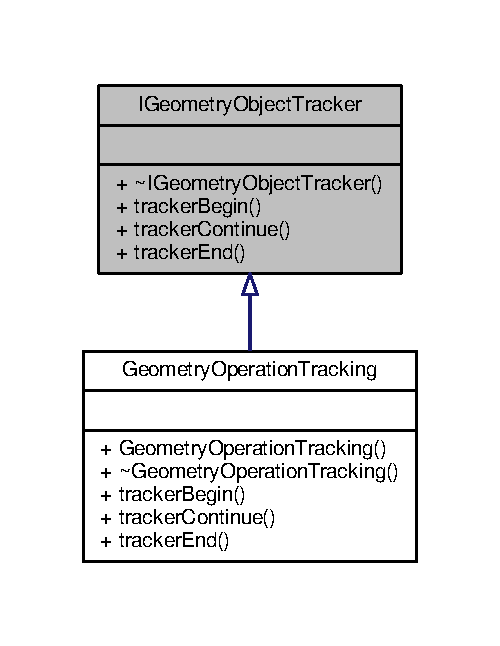
\includegraphics[width=240pt]{class_i_geometry_object_tracker__inherit__graph}
\end{center}
\end{figure}


Collaboration diagram for I\-Geometry\-Object\-Tracker\-:
\nopagebreak
\begin{figure}[H]
\begin{center}
\leavevmode
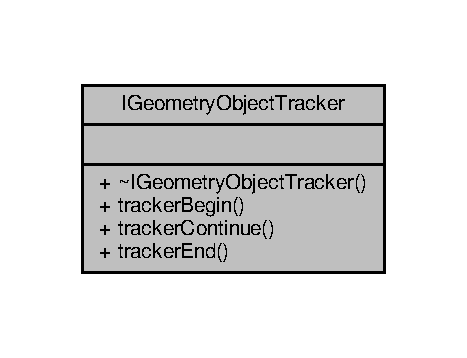
\includegraphics[width=224pt]{class_i_geometry_object_tracker__coll__graph}
\end{center}
\end{figure}
\subsection*{Public Member Functions}
\begin{DoxyCompactItemize}
\item 
virtual \hyperlink{class_i_geometry_object_tracker_a314a1e7373ba6400b91f7c2069aa9522}{$\sim$\-I\-Geometry\-Object\-Tracker} ()
\item 
virtual void \hyperlink{class_i_geometry_object_tracker_a26378a17758fe170cb8187a9e604cda4}{tracker\-Begin} (int x, int y)=0
\item 
virtual void \hyperlink{class_i_geometry_object_tracker_a2bcfcca91ae8aa0db1553bb9459c862c}{tracker\-Continue} (int x, int y)=0
\item 
virtual void \hyperlink{class_i_geometry_object_tracker_a92053b85849a8796e5ba01dba50a01fc}{tracker\-End} (int x, int y)=0
\end{DoxyCompactItemize}


\subsection{Detailed Description}


Definition at line 12 of file I\-Geometry\-Object\-Tracker.\-h.



\subsection{Constructor \& Destructor Documentation}
\hypertarget{class_i_geometry_object_tracker_a314a1e7373ba6400b91f7c2069aa9522}{\index{I\-Geometry\-Object\-Tracker@{I\-Geometry\-Object\-Tracker}!$\sim$\-I\-Geometry\-Object\-Tracker@{$\sim$\-I\-Geometry\-Object\-Tracker}}
\index{$\sim$\-I\-Geometry\-Object\-Tracker@{$\sim$\-I\-Geometry\-Object\-Tracker}!IGeometryObjectTracker@{I\-Geometry\-Object\-Tracker}}
\subsubsection[{$\sim$\-I\-Geometry\-Object\-Tracker}]{\setlength{\rightskip}{0pt plus 5cm}virtual I\-Geometry\-Object\-Tracker\-::$\sim$\-I\-Geometry\-Object\-Tracker (
\begin{DoxyParamCaption}
{}
\end{DoxyParamCaption}
)\hspace{0.3cm}{\ttfamily [inline]}, {\ttfamily [virtual]}}}\label{class_i_geometry_object_tracker_a314a1e7373ba6400b91f7c2069aa9522}


Definition at line 15 of file I\-Geometry\-Object\-Tracker.\-h.



\subsection{Member Function Documentation}
\hypertarget{class_i_geometry_object_tracker_a26378a17758fe170cb8187a9e604cda4}{\index{I\-Geometry\-Object\-Tracker@{I\-Geometry\-Object\-Tracker}!tracker\-Begin@{tracker\-Begin}}
\index{tracker\-Begin@{tracker\-Begin}!IGeometryObjectTracker@{I\-Geometry\-Object\-Tracker}}
\subsubsection[{tracker\-Begin}]{\setlength{\rightskip}{0pt plus 5cm}virtual void I\-Geometry\-Object\-Tracker\-::tracker\-Begin (
\begin{DoxyParamCaption}
\item[{int}]{x, }
\item[{int}]{y}
\end{DoxyParamCaption}
)\hspace{0.3cm}{\ttfamily [pure virtual]}}}\label{class_i_geometry_object_tracker_a26378a17758fe170cb8187a9e604cda4}


Implemented in \hyperlink{class_geometry_operation_tracking_a70bd6c4d97d234b40fd651ae8e64f11c}{Geometry\-Operation\-Tracking}.

\hypertarget{class_i_geometry_object_tracker_a2bcfcca91ae8aa0db1553bb9459c862c}{\index{I\-Geometry\-Object\-Tracker@{I\-Geometry\-Object\-Tracker}!tracker\-Continue@{tracker\-Continue}}
\index{tracker\-Continue@{tracker\-Continue}!IGeometryObjectTracker@{I\-Geometry\-Object\-Tracker}}
\subsubsection[{tracker\-Continue}]{\setlength{\rightskip}{0pt plus 5cm}virtual void I\-Geometry\-Object\-Tracker\-::tracker\-Continue (
\begin{DoxyParamCaption}
\item[{int}]{x, }
\item[{int}]{y}
\end{DoxyParamCaption}
)\hspace{0.3cm}{\ttfamily [pure virtual]}}}\label{class_i_geometry_object_tracker_a2bcfcca91ae8aa0db1553bb9459c862c}


Implemented in \hyperlink{class_geometry_operation_tracking_acc5cf88d35759c05a5e8e7ffe24ee3d6}{Geometry\-Operation\-Tracking}.

\hypertarget{class_i_geometry_object_tracker_a92053b85849a8796e5ba01dba50a01fc}{\index{I\-Geometry\-Object\-Tracker@{I\-Geometry\-Object\-Tracker}!tracker\-End@{tracker\-End}}
\index{tracker\-End@{tracker\-End}!IGeometryObjectTracker@{I\-Geometry\-Object\-Tracker}}
\subsubsection[{tracker\-End}]{\setlength{\rightskip}{0pt plus 5cm}virtual void I\-Geometry\-Object\-Tracker\-::tracker\-End (
\begin{DoxyParamCaption}
\item[{int}]{x, }
\item[{int}]{y}
\end{DoxyParamCaption}
)\hspace{0.3cm}{\ttfamily [pure virtual]}}}\label{class_i_geometry_object_tracker_a92053b85849a8796e5ba01dba50a01fc}


Implemented in \hyperlink{class_geometry_operation_tracking_ac67cebded53099bd604c4ffbef125080}{Geometry\-Operation\-Tracking}.



The documentation for this class was generated from the following file\-:\begin{DoxyCompactItemize}
\item 
\hyperlink{_i_geometry_object_tracker_8h}{I\-Geometry\-Object\-Tracker.\-h}\end{DoxyCompactItemize}

\hypertarget{class_i_view_updatable}{\section{I\-View\-Updatable Class Reference}
\label{class_i_view_updatable}\index{I\-View\-Updatable@{I\-View\-Updatable}}
}


{\ttfamily \#include $<$I\-View\-Updatable.\-h$>$}



Inheritance diagram for I\-View\-Updatable\-:\nopagebreak
\begin{figure}[H]
\begin{center}
\leavevmode
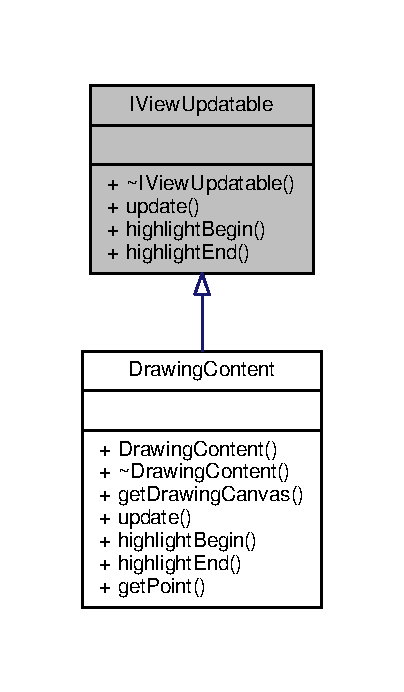
\includegraphics[width=194pt]{class_i_view_updatable__inherit__graph}
\end{center}
\end{figure}


Collaboration diagram for I\-View\-Updatable\-:
\nopagebreak
\begin{figure}[H]
\begin{center}
\leavevmode
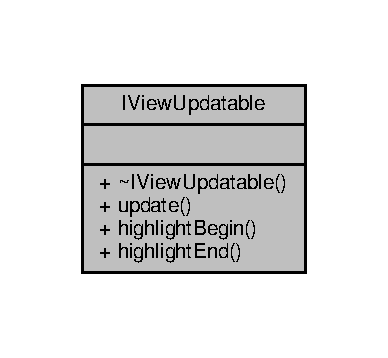
\includegraphics[width=186pt]{class_i_view_updatable__coll__graph}
\end{center}
\end{figure}
\subsection*{Public Member Functions}
\begin{DoxyCompactItemize}
\item 
virtual \hyperlink{class_i_view_updatable_a8b1b6977106371b566aa586cedca375d}{$\sim$\-I\-View\-Updatable} ()
\item 
virtual void \hyperlink{class_i_view_updatable_a7bb2c3735909fe059e5030ad3dde42ff}{update} ()=0
\item 
virtual void \hyperlink{class_i_view_updatable_aaf59f7e755222be617f6d24da32b7c47}{highlight\-Begin} (\hyperlink{class_point}{Point} \&point)=0
\item 
virtual void \hyperlink{class_i_view_updatable_a3c3f25cec4eb59d005aa229b60dc0bdf}{highlight\-End} ()=0
\end{DoxyCompactItemize}


\subsection{Detailed Description}


Definition at line 13 of file I\-View\-Updatable.\-h.



\subsection{Constructor \& Destructor Documentation}
\hypertarget{class_i_view_updatable_a8b1b6977106371b566aa586cedca375d}{\index{I\-View\-Updatable@{I\-View\-Updatable}!$\sim$\-I\-View\-Updatable@{$\sim$\-I\-View\-Updatable}}
\index{$\sim$\-I\-View\-Updatable@{$\sim$\-I\-View\-Updatable}!IViewUpdatable@{I\-View\-Updatable}}
\subsubsection[{$\sim$\-I\-View\-Updatable}]{\setlength{\rightskip}{0pt plus 5cm}virtual I\-View\-Updatable\-::$\sim$\-I\-View\-Updatable (
\begin{DoxyParamCaption}
{}
\end{DoxyParamCaption}
)\hspace{0.3cm}{\ttfamily [inline]}, {\ttfamily [virtual]}}}\label{class_i_view_updatable_a8b1b6977106371b566aa586cedca375d}


Definition at line 16 of file I\-View\-Updatable.\-h.



\subsection{Member Function Documentation}
\hypertarget{class_i_view_updatable_aaf59f7e755222be617f6d24da32b7c47}{\index{I\-View\-Updatable@{I\-View\-Updatable}!highlight\-Begin@{highlight\-Begin}}
\index{highlight\-Begin@{highlight\-Begin}!IViewUpdatable@{I\-View\-Updatable}}
\subsubsection[{highlight\-Begin}]{\setlength{\rightskip}{0pt plus 5cm}virtual void I\-View\-Updatable\-::highlight\-Begin (
\begin{DoxyParamCaption}
\item[{{\bf Point} \&}]{point}
\end{DoxyParamCaption}
)\hspace{0.3cm}{\ttfamily [pure virtual]}}}\label{class_i_view_updatable_aaf59f7e755222be617f6d24da32b7c47}


Implemented in \hyperlink{class_drawing_content_a9c9c2b7812ac5ec2cff9d9712606c8fa}{Drawing\-Content}.



Here is the caller graph for this function\-:\nopagebreak
\begin{figure}[H]
\begin{center}
\leavevmode
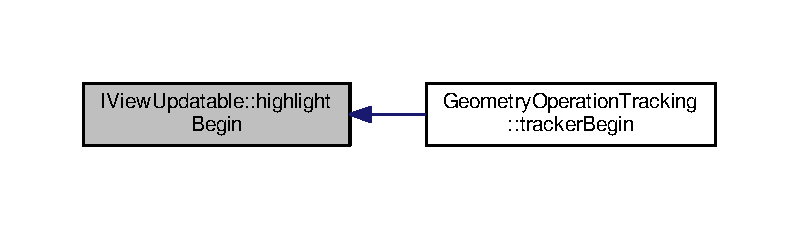
\includegraphics[width=350pt]{class_i_view_updatable_aaf59f7e755222be617f6d24da32b7c47_icgraph}
\end{center}
\end{figure}


\hypertarget{class_i_view_updatable_a3c3f25cec4eb59d005aa229b60dc0bdf}{\index{I\-View\-Updatable@{I\-View\-Updatable}!highlight\-End@{highlight\-End}}
\index{highlight\-End@{highlight\-End}!IViewUpdatable@{I\-View\-Updatable}}
\subsubsection[{highlight\-End}]{\setlength{\rightskip}{0pt plus 5cm}virtual void I\-View\-Updatable\-::highlight\-End (
\begin{DoxyParamCaption}
{}
\end{DoxyParamCaption}
)\hspace{0.3cm}{\ttfamily [pure virtual]}}}\label{class_i_view_updatable_a3c3f25cec4eb59d005aa229b60dc0bdf}


Implemented in \hyperlink{class_drawing_content_aef196b253d9057b2396d7aa0e6aa5646}{Drawing\-Content}.



Here is the caller graph for this function\-:\nopagebreak
\begin{figure}[H]
\begin{center}
\leavevmode
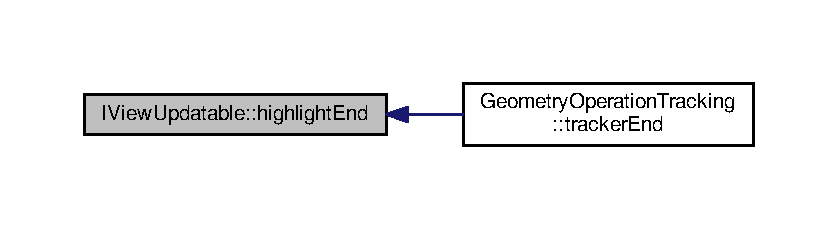
\includegraphics[width=350pt]{class_i_view_updatable_a3c3f25cec4eb59d005aa229b60dc0bdf_icgraph}
\end{center}
\end{figure}


\hypertarget{class_i_view_updatable_a7bb2c3735909fe059e5030ad3dde42ff}{\index{I\-View\-Updatable@{I\-View\-Updatable}!update@{update}}
\index{update@{update}!IViewUpdatable@{I\-View\-Updatable}}
\subsubsection[{update}]{\setlength{\rightskip}{0pt plus 5cm}virtual void I\-View\-Updatable\-::update (
\begin{DoxyParamCaption}
{}
\end{DoxyParamCaption}
)\hspace{0.3cm}{\ttfamily [pure virtual]}}}\label{class_i_view_updatable_a7bb2c3735909fe059e5030ad3dde42ff}


Implemented in \hyperlink{class_drawing_content_ae162f5d085ebdb6bd1d13bd2c895495a}{Drawing\-Content}.



Here is the caller graph for this function\-:\nopagebreak
\begin{figure}[H]
\begin{center}
\leavevmode
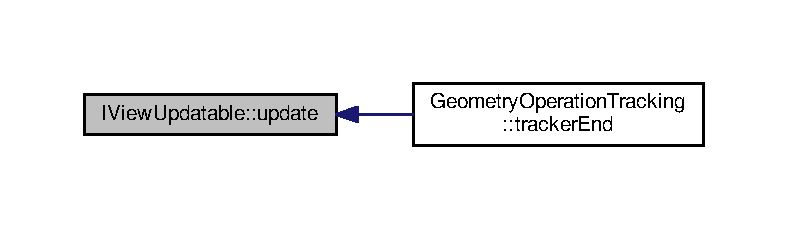
\includegraphics[width=350pt]{class_i_view_updatable_a7bb2c3735909fe059e5030ad3dde42ff_icgraph}
\end{center}
\end{figure}




The documentation for this class was generated from the following file\-:\begin{DoxyCompactItemize}
\item 
\hyperlink{_i_view_updatable_8h}{I\-View\-Updatable.\-h}\end{DoxyCompactItemize}

\hypertarget{class_i_window_listener}{\section{I\-Window\-Listener Class Reference}
\label{class_i_window_listener}\index{I\-Window\-Listener@{I\-Window\-Listener}}
}


{\ttfamily \#include $<$Window.\-h$>$}



Inheritance diagram for I\-Window\-Listener\-:\nopagebreak
\begin{figure}[H]
\begin{center}
\leavevmode
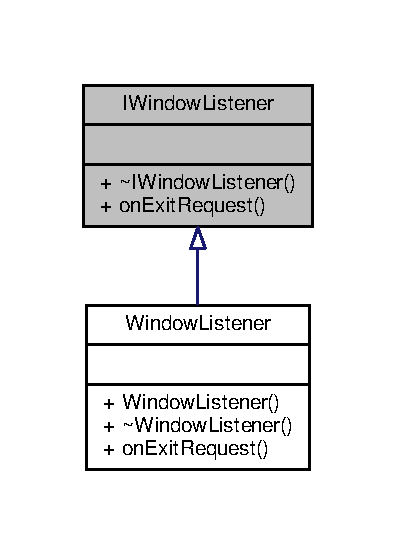
\includegraphics[width=190pt]{class_i_window_listener__inherit__graph}
\end{center}
\end{figure}


Collaboration diagram for I\-Window\-Listener\-:
\nopagebreak
\begin{figure}[H]
\begin{center}
\leavevmode
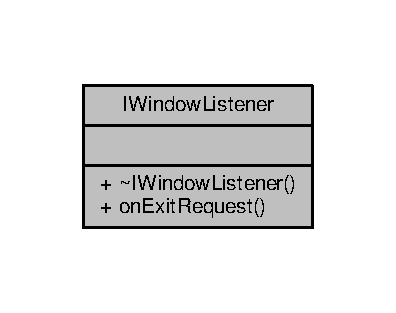
\includegraphics[width=190pt]{class_i_window_listener__coll__graph}
\end{center}
\end{figure}
\subsection*{Public Member Functions}
\begin{DoxyCompactItemize}
\item 
virtual \hyperlink{class_i_window_listener_ad7f9d263f3c12a679a61d537eda54d8d}{$\sim$\-I\-Window\-Listener} ()
\item 
virtual void \hyperlink{class_i_window_listener_ae96ae51b613e874865d985e376da01aa}{on\-Exit\-Request} (\hyperlink{class_window}{Window} \&win)=0
\end{DoxyCompactItemize}


\subsection{Detailed Description}


Definition at line 112 of file Window.\-h.



\subsection{Constructor \& Destructor Documentation}
\hypertarget{class_i_window_listener_ad7f9d263f3c12a679a61d537eda54d8d}{\index{I\-Window\-Listener@{I\-Window\-Listener}!$\sim$\-I\-Window\-Listener@{$\sim$\-I\-Window\-Listener}}
\index{$\sim$\-I\-Window\-Listener@{$\sim$\-I\-Window\-Listener}!IWindowListener@{I\-Window\-Listener}}
\subsubsection[{$\sim$\-I\-Window\-Listener}]{\setlength{\rightskip}{0pt plus 5cm}virtual I\-Window\-Listener\-::$\sim$\-I\-Window\-Listener (
\begin{DoxyParamCaption}
{}
\end{DoxyParamCaption}
)\hspace{0.3cm}{\ttfamily [inline]}, {\ttfamily [virtual]}}}\label{class_i_window_listener_ad7f9d263f3c12a679a61d537eda54d8d}


Definition at line 115 of file Window.\-h.



\subsection{Member Function Documentation}
\hypertarget{class_i_window_listener_ae96ae51b613e874865d985e376da01aa}{\index{I\-Window\-Listener@{I\-Window\-Listener}!on\-Exit\-Request@{on\-Exit\-Request}}
\index{on\-Exit\-Request@{on\-Exit\-Request}!IWindowListener@{I\-Window\-Listener}}
\subsubsection[{on\-Exit\-Request}]{\setlength{\rightskip}{0pt plus 5cm}virtual void I\-Window\-Listener\-::on\-Exit\-Request (
\begin{DoxyParamCaption}
\item[{{\bf Window} \&}]{win}
\end{DoxyParamCaption}
)\hspace{0.3cm}{\ttfamily [pure virtual]}}}\label{class_i_window_listener_ae96ae51b613e874865d985e376da01aa}
Call if user reqest close window 
\begin{DoxyParams}{Parameters}
{\em win} & ref. to \hyperlink{class_window}{Window} object \\
\hline
\end{DoxyParams}


Implemented in \hyperlink{class_window_listener_a2e4f8610046140cc051aa4fa5b609379}{Window\-Listener}.



The documentation for this class was generated from the following file\-:\begin{DoxyCompactItemize}
\item 
\hyperlink{_window_8h}{Window.\-h}\end{DoxyCompactItemize}

\hypertarget{class_main_content}{\section{Main\-Content Class Reference}
\label{class_main_content}\index{Main\-Content@{Main\-Content}}
}


{\ttfamily \#include $<$Main\-Content.\-h$>$}



Collaboration diagram for Main\-Content\-:
\nopagebreak
\begin{figure}[H]
\begin{center}
\leavevmode
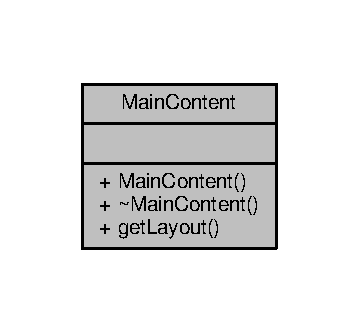
\includegraphics[width=172pt]{class_main_content__coll__graph}
\end{center}
\end{figure}
\subsection*{Public Member Functions}
\begin{DoxyCompactItemize}
\item 
\hyperlink{class_main_content_a9c13722e94a6f40d8679c54ce2f24dfc}{Main\-Content} (Evas\-\_\-\-Object $\ast$parent)
\item 
\hyperlink{class_main_content_af96ea732d30fb56c6295fa342015af3e}{$\sim$\-Main\-Content} ()
\item 
Evas\-\_\-\-Object $\ast$ \hyperlink{class_main_content_aa1917c663a7d5721e3f868eb6ae3ebe0}{get\-Layout} ()
\end{DoxyCompactItemize}


\subsection{Detailed Description}


Definition at line 13 of file Main\-Content.\-h.



\subsection{Constructor \& Destructor Documentation}
\hypertarget{class_main_content_a9c13722e94a6f40d8679c54ce2f24dfc}{\index{Main\-Content@{Main\-Content}!Main\-Content@{Main\-Content}}
\index{Main\-Content@{Main\-Content}!MainContent@{Main\-Content}}
\subsubsection[{Main\-Content}]{\setlength{\rightskip}{0pt plus 5cm}Main\-Content\-::\-Main\-Content (
\begin{DoxyParamCaption}
\item[{Evas\-\_\-\-Object $\ast$}]{parent}
\end{DoxyParamCaption}
)}}\label{class_main_content_a9c13722e94a6f40d8679c54ce2f24dfc}


Definition at line 18 of file Main\-Content.\-cpp.

\hypertarget{class_main_content_af96ea732d30fb56c6295fa342015af3e}{\index{Main\-Content@{Main\-Content}!$\sim$\-Main\-Content@{$\sim$\-Main\-Content}}
\index{$\sim$\-Main\-Content@{$\sim$\-Main\-Content}!MainContent@{Main\-Content}}
\subsubsection[{$\sim$\-Main\-Content}]{\setlength{\rightskip}{0pt plus 5cm}Main\-Content\-::$\sim$\-Main\-Content (
\begin{DoxyParamCaption}
{}
\end{DoxyParamCaption}
)}}\label{class_main_content_af96ea732d30fb56c6295fa342015af3e}


Definition at line 23 of file Main\-Content.\-cpp.



\subsection{Member Function Documentation}
\hypertarget{class_main_content_aa1917c663a7d5721e3f868eb6ae3ebe0}{\index{Main\-Content@{Main\-Content}!get\-Layout@{get\-Layout}}
\index{get\-Layout@{get\-Layout}!MainContent@{Main\-Content}}
\subsubsection[{get\-Layout}]{\setlength{\rightskip}{0pt plus 5cm}Evas\-\_\-\-Object $\ast$ Main\-Content\-::get\-Layout (
\begin{DoxyParamCaption}
{}
\end{DoxyParamCaption}
)}}\label{class_main_content_aa1917c663a7d5721e3f868eb6ae3ebe0}


Definition at line 28 of file Main\-Content.\-cpp.



The documentation for this class was generated from the following files\-:\begin{DoxyCompactItemize}
\item 
\hyperlink{_main_content_8h}{Main\-Content.\-h}\item 
\hyperlink{_main_content_8cpp}{Main\-Content.\-cpp}\end{DoxyCompactItemize}

\hypertarget{class_mouse_listener}{\section{Mouse\-Listener Class Reference}
\label{class_mouse_listener}\index{Mouse\-Listener@{Mouse\-Listener}}
}


{\ttfamily \#include $<$Mouse\-Listener.\-h$>$}



Collaboration diagram for Mouse\-Listener\-:
\nopagebreak
\begin{figure}[H]
\begin{center}
\leavevmode
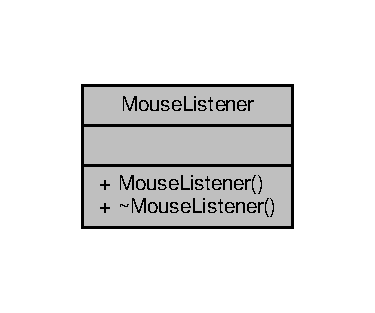
\includegraphics[width=180pt]{class_mouse_listener__coll__graph}
\end{center}
\end{figure}
\subsection*{Public Member Functions}
\begin{DoxyCompactItemize}
\item 
\hyperlink{class_mouse_listener_a0710a904e084b30269fd958ed36f82e4}{Mouse\-Listener} (\hyperlink{class_i_geometry_object_tracker}{I\-Geometry\-Object\-Tracker} \&geo\-Object\-Tracker, Evas\-\_\-\-Object $\ast$canvas)
\item 
virtual \hyperlink{class_mouse_listener_accd4936ce82d935281544d9d1b61fb7d}{$\sim$\-Mouse\-Listener} ()
\end{DoxyCompactItemize}


\subsection{Detailed Description}


Definition at line 14 of file Mouse\-Listener.\-h.



\subsection{Constructor \& Destructor Documentation}
\hypertarget{class_mouse_listener_a0710a904e084b30269fd958ed36f82e4}{\index{Mouse\-Listener@{Mouse\-Listener}!Mouse\-Listener@{Mouse\-Listener}}
\index{Mouse\-Listener@{Mouse\-Listener}!MouseListener@{Mouse\-Listener}}
\subsubsection[{Mouse\-Listener}]{\setlength{\rightskip}{0pt plus 5cm}Mouse\-Listener\-::\-Mouse\-Listener (
\begin{DoxyParamCaption}
\item[{{\bf I\-Geometry\-Object\-Tracker} \&}]{geo\-Object\-Tracker, }
\item[{Evas\-\_\-\-Object $\ast$}]{canvas}
\end{DoxyParamCaption}
)}}\label{class_mouse_listener_a0710a904e084b30269fd958ed36f82e4}


Definition at line 12 of file Mouse\-Listener.\-cpp.

\hypertarget{class_mouse_listener_accd4936ce82d935281544d9d1b61fb7d}{\index{Mouse\-Listener@{Mouse\-Listener}!$\sim$\-Mouse\-Listener@{$\sim$\-Mouse\-Listener}}
\index{$\sim$\-Mouse\-Listener@{$\sim$\-Mouse\-Listener}!MouseListener@{Mouse\-Listener}}
\subsubsection[{$\sim$\-Mouse\-Listener}]{\setlength{\rightskip}{0pt plus 5cm}Mouse\-Listener\-::$\sim$\-Mouse\-Listener (
\begin{DoxyParamCaption}
{}
\end{DoxyParamCaption}
)\hspace{0.3cm}{\ttfamily [virtual]}}}\label{class_mouse_listener_accd4936ce82d935281544d9d1b61fb7d}


Definition at line 20 of file Mouse\-Listener.\-cpp.



The documentation for this class was generated from the following files\-:\begin{DoxyCompactItemize}
\item 
\hyperlink{_mouse_listener_8h}{Mouse\-Listener.\-h}\item 
\hyperlink{_mouse_listener_8cpp}{Mouse\-Listener.\-cpp}\end{DoxyCompactItemize}

\hypertarget{class_point}{\section{Point Class Reference}
\label{class_point}\index{Point@{Point}}
}


{\ttfamily \#include $<$Point.\-h$>$}



Inheritance diagram for Point\-:\nopagebreak
\begin{figure}[H]
\begin{center}
\leavevmode
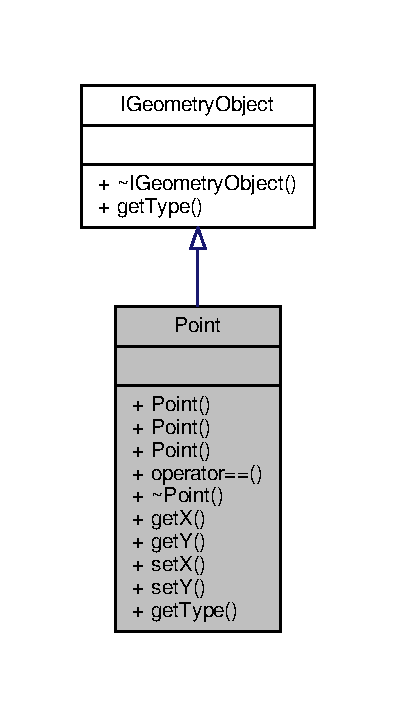
\includegraphics[width=190pt]{class_point__inherit__graph}
\end{center}
\end{figure}


Collaboration diagram for Point\-:
\nopagebreak
\begin{figure}[H]
\begin{center}
\leavevmode
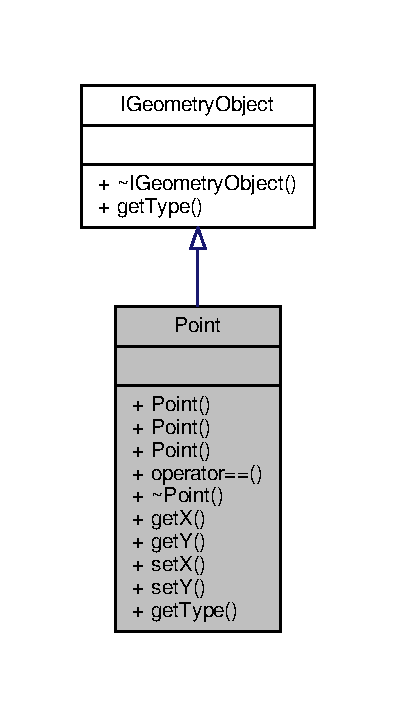
\includegraphics[width=190pt]{class_point__coll__graph}
\end{center}
\end{figure}
\subsection*{Public Member Functions}
\begin{DoxyCompactItemize}
\item 
\hyperlink{class_point_ad92f2337b839a94ce97dcdb439b4325a}{Point} ()
\item 
\hyperlink{class_point_a001c4958c310b248f5c26037aea38a9c}{Point} (int x, int y)
\item 
\hyperlink{class_point_a7485d0952c4bf845fc02bb1a75cbdcc1}{Point} (const \hyperlink{class_point}{Point} \&src)
\item 
bool \hyperlink{class_point_a7ee89c9b4947cf4f983d7dd227bfd56c}{operator==} (\hyperlink{class_point}{Point} \&src)
\item 
virtual \hyperlink{class_point_a395fa04b4ec126b66fc053f829a30cc1}{$\sim$\-Point} ()
\item 
int \hyperlink{class_point_a0b82a4aa9614c11854abc507d89a70a9}{get\-X} ()
\item 
int \hyperlink{class_point_a3770f321c49dfe7ca463900fddc2e2bc}{get\-Y} ()
\item 
void \hyperlink{class_point_acdc86ab607b2ae8415152883e2629015}{set\-X} (int x)
\item 
void \hyperlink{class_point_afccad787a359f062efc1af5e935a99ba}{set\-Y} (int y)
\item 
\hyperlink{_geometry_objects_types_8h_adea8b8c3a289ca1fc1450d9424dcd33d}{Geometry\-Objects\-Types} \hyperlink{class_point_a87134ba772c2c01168a996a849214955}{get\-Type} ()
\end{DoxyCompactItemize}


\subsection{Detailed Description}


Definition at line 13 of file Point.\-h.



\subsection{Constructor \& Destructor Documentation}
\hypertarget{class_point_ad92f2337b839a94ce97dcdb439b4325a}{\index{Point@{Point}!Point@{Point}}
\index{Point@{Point}!Point@{Point}}
\subsubsection[{Point}]{\setlength{\rightskip}{0pt plus 5cm}Point\-::\-Point (
\begin{DoxyParamCaption}
{}
\end{DoxyParamCaption}
)}}\label{class_point_ad92f2337b839a94ce97dcdb439b4325a}


Definition at line 10 of file Point.\-cpp.

\hypertarget{class_point_a001c4958c310b248f5c26037aea38a9c}{\index{Point@{Point}!Point@{Point}}
\index{Point@{Point}!Point@{Point}}
\subsubsection[{Point}]{\setlength{\rightskip}{0pt plus 5cm}Point\-::\-Point (
\begin{DoxyParamCaption}
\item[{int}]{x, }
\item[{int}]{y}
\end{DoxyParamCaption}
)}}\label{class_point_a001c4958c310b248f5c26037aea38a9c}


Definition at line 15 of file Point.\-cpp.

\hypertarget{class_point_a7485d0952c4bf845fc02bb1a75cbdcc1}{\index{Point@{Point}!Point@{Point}}
\index{Point@{Point}!Point@{Point}}
\subsubsection[{Point}]{\setlength{\rightskip}{0pt plus 5cm}Point\-::\-Point (
\begin{DoxyParamCaption}
\item[{const {\bf Point} \&}]{src}
\end{DoxyParamCaption}
)}}\label{class_point_a7485d0952c4bf845fc02bb1a75cbdcc1}


Definition at line 20 of file Point.\-cpp.

\hypertarget{class_point_a395fa04b4ec126b66fc053f829a30cc1}{\index{Point@{Point}!$\sim$\-Point@{$\sim$\-Point}}
\index{$\sim$\-Point@{$\sim$\-Point}!Point@{Point}}
\subsubsection[{$\sim$\-Point}]{\setlength{\rightskip}{0pt plus 5cm}Point\-::$\sim$\-Point (
\begin{DoxyParamCaption}
{}
\end{DoxyParamCaption}
)\hspace{0.3cm}{\ttfamily [virtual]}}}\label{class_point_a395fa04b4ec126b66fc053f829a30cc1}


Definition at line 39 of file Point.\-cpp.



\subsection{Member Function Documentation}
\hypertarget{class_point_a87134ba772c2c01168a996a849214955}{\index{Point@{Point}!get\-Type@{get\-Type}}
\index{get\-Type@{get\-Type}!Point@{Point}}
\subsubsection[{get\-Type}]{\setlength{\rightskip}{0pt plus 5cm}{\bf Geometry\-Objects\-Types} Point\-::get\-Type (
\begin{DoxyParamCaption}
{}
\end{DoxyParamCaption}
)\hspace{0.3cm}{\ttfamily [virtual]}}}\label{class_point_a87134ba772c2c01168a996a849214955}


Implements \hyperlink{class_i_geometry_object_ae88064004986a5d599f5794fc3eefca3}{I\-Geometry\-Object}.



Definition at line 63 of file Point.\-cpp.

\hypertarget{class_point_a0b82a4aa9614c11854abc507d89a70a9}{\index{Point@{Point}!get\-X@{get\-X}}
\index{get\-X@{get\-X}!Point@{Point}}
\subsubsection[{get\-X}]{\setlength{\rightskip}{0pt plus 5cm}int Point\-::get\-X (
\begin{DoxyParamCaption}
{}
\end{DoxyParamCaption}
)}}\label{class_point_a0b82a4aa9614c11854abc507d89a70a9}


Definition at line 43 of file Point.\-cpp.



Here is the caller graph for this function\-:\nopagebreak
\begin{figure}[H]
\begin{center}
\leavevmode
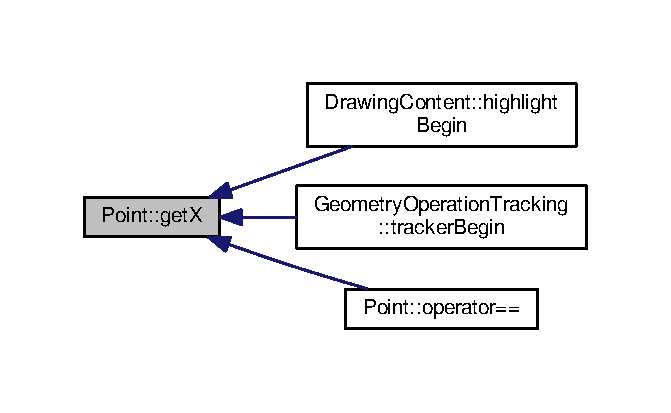
\includegraphics[width=322pt]{class_point_a0b82a4aa9614c11854abc507d89a70a9_icgraph}
\end{center}
\end{figure}


\hypertarget{class_point_a3770f321c49dfe7ca463900fddc2e2bc}{\index{Point@{Point}!get\-Y@{get\-Y}}
\index{get\-Y@{get\-Y}!Point@{Point}}
\subsubsection[{get\-Y}]{\setlength{\rightskip}{0pt plus 5cm}int Point\-::get\-Y (
\begin{DoxyParamCaption}
{}
\end{DoxyParamCaption}
)}}\label{class_point_a3770f321c49dfe7ca463900fddc2e2bc}


Definition at line 48 of file Point.\-cpp.



Here is the caller graph for this function\-:\nopagebreak
\begin{figure}[H]
\begin{center}
\leavevmode
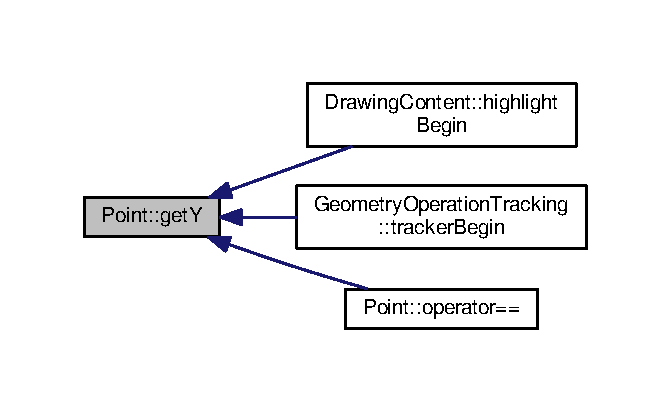
\includegraphics[width=322pt]{class_point_a3770f321c49dfe7ca463900fddc2e2bc_icgraph}
\end{center}
\end{figure}


\hypertarget{class_point_a7ee89c9b4947cf4f983d7dd227bfd56c}{\index{Point@{Point}!operator==@{operator==}}
\index{operator==@{operator==}!Point@{Point}}
\subsubsection[{operator==}]{\setlength{\rightskip}{0pt plus 5cm}bool Point\-::operator== (
\begin{DoxyParamCaption}
\item[{{\bf Point} \&}]{src}
\end{DoxyParamCaption}
)}}\label{class_point_a7ee89c9b4947cf4f983d7dd227bfd56c}


Definition at line 26 of file Point.\-cpp.



Here is the call graph for this function\-:\nopagebreak
\begin{figure}[H]
\begin{center}
\leavevmode
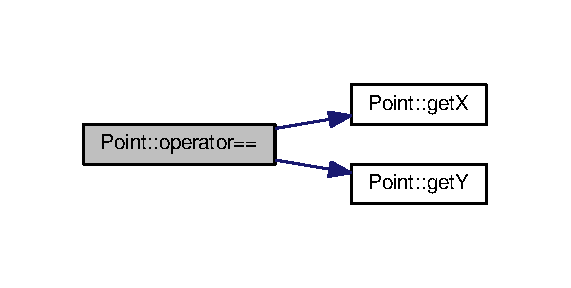
\includegraphics[width=274pt]{class_point_a7ee89c9b4947cf4f983d7dd227bfd56c_cgraph}
\end{center}
\end{figure}


\hypertarget{class_point_acdc86ab607b2ae8415152883e2629015}{\index{Point@{Point}!set\-X@{set\-X}}
\index{set\-X@{set\-X}!Point@{Point}}
\subsubsection[{set\-X}]{\setlength{\rightskip}{0pt plus 5cm}void Point\-::set\-X (
\begin{DoxyParamCaption}
\item[{int}]{x}
\end{DoxyParamCaption}
)}}\label{class_point_acdc86ab607b2ae8415152883e2629015}


Definition at line 53 of file Point.\-cpp.

\hypertarget{class_point_afccad787a359f062efc1af5e935a99ba}{\index{Point@{Point}!set\-Y@{set\-Y}}
\index{set\-Y@{set\-Y}!Point@{Point}}
\subsubsection[{set\-Y}]{\setlength{\rightskip}{0pt plus 5cm}void Point\-::set\-Y (
\begin{DoxyParamCaption}
\item[{int}]{y}
\end{DoxyParamCaption}
)}}\label{class_point_afccad787a359f062efc1af5e935a99ba}


Definition at line 58 of file Point.\-cpp.



The documentation for this class was generated from the following files\-:\begin{DoxyCompactItemize}
\item 
\hyperlink{_point_8h}{Point.\-h}\item 
\hyperlink{_point_8cpp}{Point.\-cpp}\end{DoxyCompactItemize}

\hypertarget{class_points_link}{\section{Points\-Link Class Reference}
\label{class_points_link}\index{Points\-Link@{Points\-Link}}
}


{\ttfamily \#include $<$Points\-Link.\-h$>$}



Inheritance diagram for Points\-Link\-:\nopagebreak
\begin{figure}[H]
\begin{center}
\leavevmode
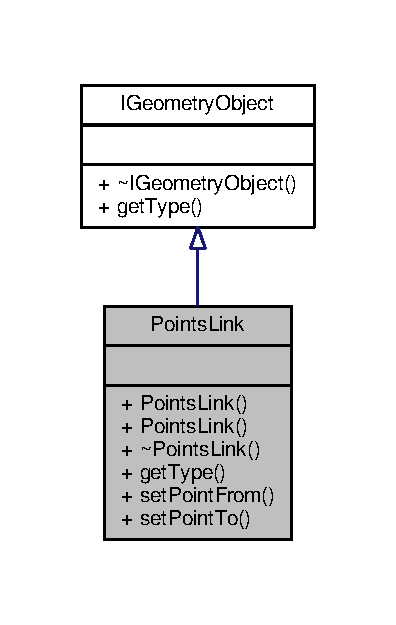
\includegraphics[width=190pt]{class_points_link__inherit__graph}
\end{center}
\end{figure}


Collaboration diagram for Points\-Link\-:
\nopagebreak
\begin{figure}[H]
\begin{center}
\leavevmode
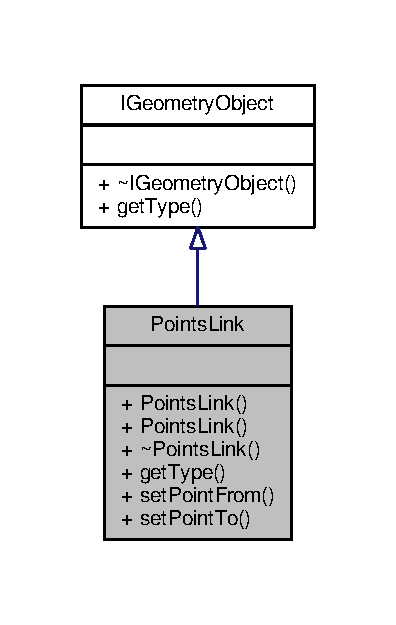
\includegraphics[width=190pt]{class_points_link__coll__graph}
\end{center}
\end{figure}
\subsection*{Public Member Functions}
\begin{DoxyCompactItemize}
\item 
\hyperlink{class_points_link_a30aadb6817dd5d1aa84bde68c87aee16}{Points\-Link} ()
\item 
\hyperlink{class_points_link_a1fd145b672d302bdd58298a2561199c4}{Points\-Link} (\hyperlink{class_point}{Point} \&point\-\_\-1, \hyperlink{class_point}{Point} \&point\-\_\-2)
\item 
virtual \hyperlink{class_points_link_a2ebcfa8b0e25d50fb72a51f458b3226f}{$\sim$\-Points\-Link} ()
\item 
\hyperlink{_geometry_objects_types_8h_adea8b8c3a289ca1fc1450d9424dcd33d}{Geometry\-Objects\-Types} \hyperlink{class_points_link_a75fcf55b27002a8f1a8db18007fc85b1}{get\-Type} ()
\item 
void \hyperlink{class_points_link_a033aaf418b2c62ad661d41b88d456387}{set\-Point\-From} (\hyperlink{class_point}{Point} \&point)
\item 
void \hyperlink{class_points_link_aa12b875826ea699987858da52c89249c}{set\-Point\-To} (\hyperlink{class_point}{Point} \&point)
\end{DoxyCompactItemize}


\subsection{Detailed Description}


Definition at line 16 of file Points\-Link.\-h.



\subsection{Constructor \& Destructor Documentation}
\hypertarget{class_points_link_a30aadb6817dd5d1aa84bde68c87aee16}{\index{Points\-Link@{Points\-Link}!Points\-Link@{Points\-Link}}
\index{Points\-Link@{Points\-Link}!PointsLink@{Points\-Link}}
\subsubsection[{Points\-Link}]{\setlength{\rightskip}{0pt plus 5cm}Points\-Link\-::\-Points\-Link (
\begin{DoxyParamCaption}
{}
\end{DoxyParamCaption}
)}}\label{class_points_link_a30aadb6817dd5d1aa84bde68c87aee16}


Definition at line 10 of file Points\-Link.\-cpp.

\hypertarget{class_points_link_a1fd145b672d302bdd58298a2561199c4}{\index{Points\-Link@{Points\-Link}!Points\-Link@{Points\-Link}}
\index{Points\-Link@{Points\-Link}!PointsLink@{Points\-Link}}
\subsubsection[{Points\-Link}]{\setlength{\rightskip}{0pt plus 5cm}Points\-Link\-::\-Points\-Link (
\begin{DoxyParamCaption}
\item[{{\bf Point} \&}]{point\-\_\-1, }
\item[{{\bf Point} \&}]{point\-\_\-2}
\end{DoxyParamCaption}
)}}\label{class_points_link_a1fd145b672d302bdd58298a2561199c4}


Definition at line 15 of file Points\-Link.\-cpp.

\hypertarget{class_points_link_a2ebcfa8b0e25d50fb72a51f458b3226f}{\index{Points\-Link@{Points\-Link}!$\sim$\-Points\-Link@{$\sim$\-Points\-Link}}
\index{$\sim$\-Points\-Link@{$\sim$\-Points\-Link}!PointsLink@{Points\-Link}}
\subsubsection[{$\sim$\-Points\-Link}]{\setlength{\rightskip}{0pt plus 5cm}Points\-Link\-::$\sim$\-Points\-Link (
\begin{DoxyParamCaption}
{}
\end{DoxyParamCaption}
)\hspace{0.3cm}{\ttfamily [virtual]}}}\label{class_points_link_a2ebcfa8b0e25d50fb72a51f458b3226f}


Definition at line 21 of file Points\-Link.\-cpp.



\subsection{Member Function Documentation}
\hypertarget{class_points_link_a75fcf55b27002a8f1a8db18007fc85b1}{\index{Points\-Link@{Points\-Link}!get\-Type@{get\-Type}}
\index{get\-Type@{get\-Type}!PointsLink@{Points\-Link}}
\subsubsection[{get\-Type}]{\setlength{\rightskip}{0pt plus 5cm}{\bf Geometry\-Objects\-Types} Points\-Link\-::get\-Type (
\begin{DoxyParamCaption}
{}
\end{DoxyParamCaption}
)\hspace{0.3cm}{\ttfamily [virtual]}}}\label{class_points_link_a75fcf55b27002a8f1a8db18007fc85b1}


Implements \hyperlink{class_i_geometry_object_ae88064004986a5d599f5794fc3eefca3}{I\-Geometry\-Object}.



Definition at line 25 of file Points\-Link.\-cpp.

\hypertarget{class_points_link_a033aaf418b2c62ad661d41b88d456387}{\index{Points\-Link@{Points\-Link}!set\-Point\-From@{set\-Point\-From}}
\index{set\-Point\-From@{set\-Point\-From}!PointsLink@{Points\-Link}}
\subsubsection[{set\-Point\-From}]{\setlength{\rightskip}{0pt plus 5cm}void Points\-Link\-::set\-Point\-From (
\begin{DoxyParamCaption}
\item[{{\bf Point} \&}]{point}
\end{DoxyParamCaption}
)}}\label{class_points_link_a033aaf418b2c62ad661d41b88d456387}


Definition at line 30 of file Points\-Link.\-cpp.

\hypertarget{class_points_link_aa12b875826ea699987858da52c89249c}{\index{Points\-Link@{Points\-Link}!set\-Point\-To@{set\-Point\-To}}
\index{set\-Point\-To@{set\-Point\-To}!PointsLink@{Points\-Link}}
\subsubsection[{set\-Point\-To}]{\setlength{\rightskip}{0pt plus 5cm}void Points\-Link\-::set\-Point\-To (
\begin{DoxyParamCaption}
\item[{{\bf Point} \&}]{point}
\end{DoxyParamCaption}
)}}\label{class_points_link_aa12b875826ea699987858da52c89249c}


Definition at line 35 of file Points\-Link.\-cpp.



The documentation for this class was generated from the following files\-:\begin{DoxyCompactItemize}
\item 
\hyperlink{_points_link_8h}{Points\-Link.\-h}\item 
\hyperlink{_points_link_8cpp}{Points\-Link.\-cpp}\end{DoxyCompactItemize}

\hypertarget{class_toolbar_content}{\section{Toolbar\-Content Class Reference}
\label{class_toolbar_content}\index{Toolbar\-Content@{Toolbar\-Content}}
}


{\ttfamily \#include $<$Toolbar\-Content.\-h$>$}



Collaboration diagram for Toolbar\-Content\-:
\nopagebreak
\begin{figure}[H]
\begin{center}
\leavevmode
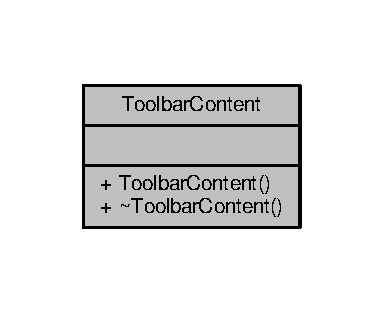
\includegraphics[width=184pt]{class_toolbar_content__coll__graph}
\end{center}
\end{figure}
\subsection*{Public Member Functions}
\begin{DoxyCompactItemize}
\item 
\hyperlink{class_toolbar_content_a8b8a2cee113baa40ca627bed75cc31d3}{Toolbar\-Content} (Evas\-\_\-\-Object $\ast$parent)
\item 
virtual \hyperlink{class_toolbar_content_a0c36bbfa7661875937f02807f9f4f16f}{$\sim$\-Toolbar\-Content} ()
\end{DoxyCompactItemize}


\subsection{Detailed Description}


Definition at line 13 of file Toolbar\-Content.\-h.



\subsection{Constructor \& Destructor Documentation}
\hypertarget{class_toolbar_content_a8b8a2cee113baa40ca627bed75cc31d3}{\index{Toolbar\-Content@{Toolbar\-Content}!Toolbar\-Content@{Toolbar\-Content}}
\index{Toolbar\-Content@{Toolbar\-Content}!ToolbarContent@{Toolbar\-Content}}
\subsubsection[{Toolbar\-Content}]{\setlength{\rightskip}{0pt plus 5cm}Toolbar\-Content\-::\-Toolbar\-Content (
\begin{DoxyParamCaption}
\item[{Evas\-\_\-\-Object $\ast$}]{parent}
\end{DoxyParamCaption}
)}}\label{class_toolbar_content_a8b8a2cee113baa40ca627bed75cc31d3}


Definition at line 16 of file Toolbar\-Content.\-cpp.

\hypertarget{class_toolbar_content_a0c36bbfa7661875937f02807f9f4f16f}{\index{Toolbar\-Content@{Toolbar\-Content}!$\sim$\-Toolbar\-Content@{$\sim$\-Toolbar\-Content}}
\index{$\sim$\-Toolbar\-Content@{$\sim$\-Toolbar\-Content}!ToolbarContent@{Toolbar\-Content}}
\subsubsection[{$\sim$\-Toolbar\-Content}]{\setlength{\rightskip}{0pt plus 5cm}Toolbar\-Content\-::$\sim$\-Toolbar\-Content (
\begin{DoxyParamCaption}
{}
\end{DoxyParamCaption}
)\hspace{0.3cm}{\ttfamily [virtual]}}}\label{class_toolbar_content_a0c36bbfa7661875937f02807f9f4f16f}


Definition at line 24 of file Toolbar\-Content.\-cpp.



The documentation for this class was generated from the following files\-:\begin{DoxyCompactItemize}
\item 
\hyperlink{_toolbar_content_8h}{Toolbar\-Content.\-h}\item 
\hyperlink{_toolbar_content_8cpp}{Toolbar\-Content.\-cpp}\end{DoxyCompactItemize}

\hypertarget{class_window}{\section{Window Class Reference}
\label{class_window}\index{Window@{Window}}
}


{\ttfamily \#include $<$Window.\-h$>$}



Inheritance diagram for Window\-:\nopagebreak
\begin{figure}[H]
\begin{center}
\leavevmode
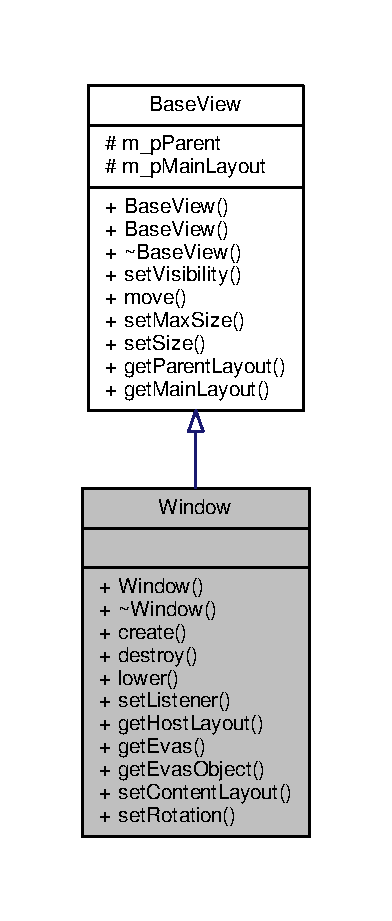
\includegraphics[width=188pt]{class_window__inherit__graph}
\end{center}
\end{figure}


Collaboration diagram for Window\-:
\nopagebreak
\begin{figure}[H]
\begin{center}
\leavevmode
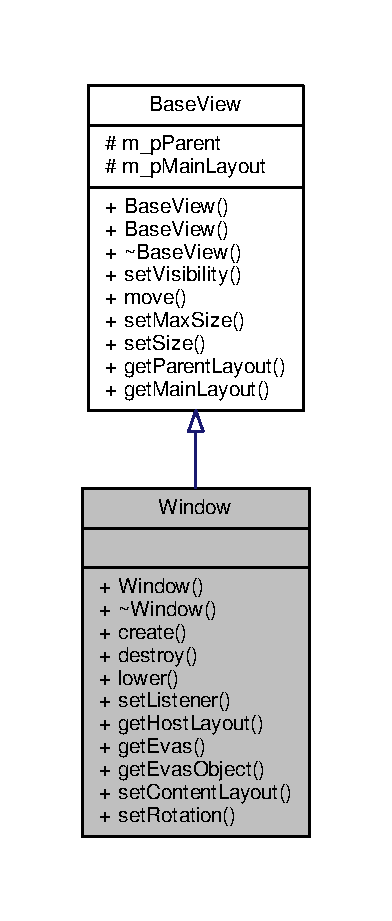
\includegraphics[width=188pt]{class_window__coll__graph}
\end{center}
\end{figure}
\subsection*{Public Member Functions}
\begin{DoxyCompactItemize}
\item 
\hyperlink{class_window_a74e6087da23d3c24e9fac0245e5ec92c}{Window} ()
\item 
virtual \hyperlink{class_window_a245d821e6016fa1f6970ccbbedd635f6}{$\sim$\-Window} ()
\item 
bool \hyperlink{class_window_a7800222f6ccedd6203126ecc9047b884}{create} ()
\item 
void \hyperlink{class_window_aa89262ad2538473c8d7e4d8dd641849d}{destroy} ()
\item 
void \hyperlink{class_window_a1cadc8b2dbfd05d10910ad53315354d1}{lower} ()
\item 
void \hyperlink{class_window_aefe72579d0c1b8308f7c0a5019eecd30}{set\-Listener} (\hyperlink{class_i_window_listener}{I\-Window\-Listener} $\ast$listener)
\item 
Evas\-\_\-\-Object $\ast$ \hyperlink{class_window_a42320edec04f8ac1d2d30c1e825ba54b}{get\-Host\-Layout} () const 
\item 
Evas $\ast$ \hyperlink{class_window_a6392b9bfee006c3152e053c998c89f85}{get\-Evas} () const 
\item 
Evas\-\_\-\-Object $\ast$ \hyperlink{class_window_a241ade30878ce1086b5cf31d117bbdc8}{get\-Evas\-Object} () const 
\item 
void \hyperlink{class_window_a65083355da28c011ece7a82011e1ec0c}{set\-Content\-Layout} (Evas\-\_\-\-Object $\ast$content)
\item 
void \hyperlink{class_window_a550a3c5b830d843e9fc3864105eb0127}{set\-Rotation} (int rotation)
\end{DoxyCompactItemize}
\subsection*{Additional Inherited Members}


\subsection{Detailed Description}


Definition at line 35 of file Window.\-h.



\subsection{Constructor \& Destructor Documentation}
\hypertarget{class_window_a74e6087da23d3c24e9fac0245e5ec92c}{\index{Window@{Window}!Window@{Window}}
\index{Window@{Window}!Window@{Window}}
\subsubsection[{Window}]{\setlength{\rightskip}{0pt plus 5cm}Window\-::\-Window (
\begin{DoxyParamCaption}
{}
\end{DoxyParamCaption}
)}}\label{class_window_a74e6087da23d3c24e9fac0245e5ec92c}
Constructor 

Definition at line 32 of file Window.\-cpp.

\hypertarget{class_window_a245d821e6016fa1f6970ccbbedd635f6}{\index{Window@{Window}!$\sim$\-Window@{$\sim$\-Window}}
\index{$\sim$\-Window@{$\sim$\-Window}!Window@{Window}}
\subsubsection[{$\sim$\-Window}]{\setlength{\rightskip}{0pt plus 5cm}Window\-::$\sim$\-Window (
\begin{DoxyParamCaption}
{}
\end{DoxyParamCaption}
)\hspace{0.3cm}{\ttfamily [virtual]}}}\label{class_window_a245d821e6016fa1f6970ccbbedd635f6}
Destructor 

Definition at line 41 of file Window.\-cpp.



Here is the call graph for this function\-:\nopagebreak
\begin{figure}[H]
\begin{center}
\leavevmode
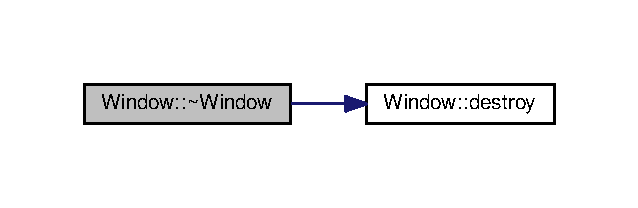
\includegraphics[width=306pt]{class_window_a245d821e6016fa1f6970ccbbedd635f6_cgraph}
\end{center}
\end{figure}




\subsection{Member Function Documentation}
\hypertarget{class_window_a7800222f6ccedd6203126ecc9047b884}{\index{Window@{Window}!create@{create}}
\index{create@{create}!Window@{Window}}
\subsubsection[{create}]{\setlength{\rightskip}{0pt plus 5cm}bool Window\-::create (
\begin{DoxyParamCaption}
{}
\end{DoxyParamCaption}
)}}\label{class_window_a7800222f6ccedd6203126ecc9047b884}
Create window 

Definition at line 46 of file Window.\-cpp.



Here is the caller graph for this function\-:\nopagebreak
\begin{figure}[H]
\begin{center}
\leavevmode
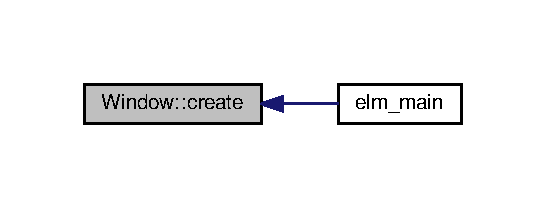
\includegraphics[width=262pt]{class_window_a7800222f6ccedd6203126ecc9047b884_icgraph}
\end{center}
\end{figure}


\hypertarget{class_window_aa89262ad2538473c8d7e4d8dd641849d}{\index{Window@{Window}!destroy@{destroy}}
\index{destroy@{destroy}!Window@{Window}}
\subsubsection[{destroy}]{\setlength{\rightskip}{0pt plus 5cm}void Window\-::destroy (
\begin{DoxyParamCaption}
{}
\end{DoxyParamCaption}
)}}\label{class_window_aa89262ad2538473c8d7e4d8dd641849d}
Destroy window 

Definition at line 79 of file Window.\-cpp.



Here is the caller graph for this function\-:\nopagebreak
\begin{figure}[H]
\begin{center}
\leavevmode
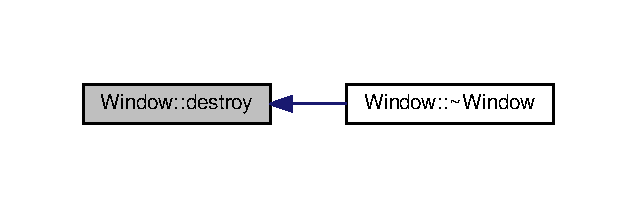
\includegraphics[width=306pt]{class_window_aa89262ad2538473c8d7e4d8dd641849d_icgraph}
\end{center}
\end{figure}


\hypertarget{class_window_a6392b9bfee006c3152e053c998c89f85}{\index{Window@{Window}!get\-Evas@{get\-Evas}}
\index{get\-Evas@{get\-Evas}!Window@{Window}}
\subsubsection[{get\-Evas}]{\setlength{\rightskip}{0pt plus 5cm}Evas $\ast$ Window\-::get\-Evas (
\begin{DoxyParamCaption}
{}
\end{DoxyParamCaption}
) const}}\label{class_window_a6392b9bfee006c3152e053c998c89f85}
Get canvas \begin{DoxyReturn}{Returns}
canvas 
\end{DoxyReturn}


Definition at line 99 of file Window.\-cpp.

\hypertarget{class_window_a241ade30878ce1086b5cf31d117bbdc8}{\index{Window@{Window}!get\-Evas\-Object@{get\-Evas\-Object}}
\index{get\-Evas\-Object@{get\-Evas\-Object}!Window@{Window}}
\subsubsection[{get\-Evas\-Object}]{\setlength{\rightskip}{0pt plus 5cm}Evas\-\_\-\-Object $\ast$ Window\-::get\-Evas\-Object (
\begin{DoxyParamCaption}
{}
\end{DoxyParamCaption}
) const}}\label{class_window_a241ade30878ce1086b5cf31d117bbdc8}
Get canvas object \begin{DoxyReturn}{Returns}
canvas object 
\end{DoxyReturn}


Definition at line 104 of file Window.\-cpp.



Here is the caller graph for this function\-:\nopagebreak
\begin{figure}[H]
\begin{center}
\leavevmode
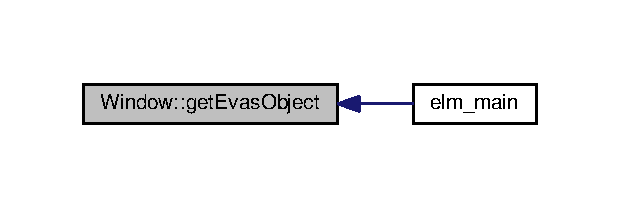
\includegraphics[width=298pt]{class_window_a241ade30878ce1086b5cf31d117bbdc8_icgraph}
\end{center}
\end{figure}


\hypertarget{class_window_a42320edec04f8ac1d2d30c1e825ba54b}{\index{Window@{Window}!get\-Host\-Layout@{get\-Host\-Layout}}
\index{get\-Host\-Layout@{get\-Host\-Layout}!Window@{Window}}
\subsubsection[{get\-Host\-Layout}]{\setlength{\rightskip}{0pt plus 5cm}Evas\-\_\-\-Object $\ast$ Window\-::get\-Host\-Layout (
\begin{DoxyParamCaption}
{}
\end{DoxyParamCaption}
) const}}\label{class_window_a42320edec04f8ac1d2d30c1e825ba54b}
Get host layout \begin{DoxyReturn}{Returns}
host Evas\-\_\-\-Object 
\end{DoxyReturn}


Definition at line 94 of file Window.\-cpp.

\hypertarget{class_window_a1cadc8b2dbfd05d10910ad53315354d1}{\index{Window@{Window}!lower@{lower}}
\index{lower@{lower}!Window@{Window}}
\subsubsection[{lower}]{\setlength{\rightskip}{0pt plus 5cm}void Window\-::lower (
\begin{DoxyParamCaption}
{}
\end{DoxyParamCaption}
)}}\label{class_window_a1cadc8b2dbfd05d10910ad53315354d1}
Lowe the window 

Definition at line 88 of file Window.\-cpp.

\hypertarget{class_window_a65083355da28c011ece7a82011e1ec0c}{\index{Window@{Window}!set\-Content\-Layout@{set\-Content\-Layout}}
\index{set\-Content\-Layout@{set\-Content\-Layout}!Window@{Window}}
\subsubsection[{set\-Content\-Layout}]{\setlength{\rightskip}{0pt plus 5cm}void Window\-::set\-Content\-Layout (
\begin{DoxyParamCaption}
\item[{Evas\-\_\-\-Object $\ast$}]{content}
\end{DoxyParamCaption}
)}}\label{class_window_a65083355da28c011ece7a82011e1ec0c}
Set or unset content 
\begin{DoxyParams}{Parameters}
{\em layout} & -\/ content layout \\
\hline
\end{DoxyParams}


Definition at line 121 of file Window.\-cpp.



Here is the caller graph for this function\-:\nopagebreak
\begin{figure}[H]
\begin{center}
\leavevmode
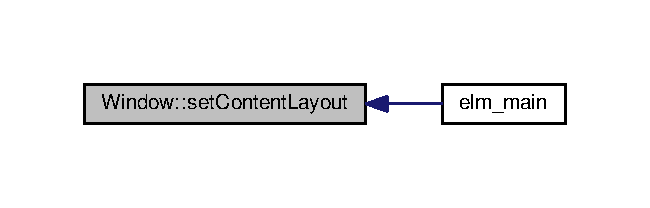
\includegraphics[width=312pt]{class_window_a65083355da28c011ece7a82011e1ec0c_icgraph}
\end{center}
\end{figure}


\hypertarget{class_window_aefe72579d0c1b8308f7c0a5019eecd30}{\index{Window@{Window}!set\-Listener@{set\-Listener}}
\index{set\-Listener@{set\-Listener}!Window@{Window}}
\subsubsection[{set\-Listener}]{\setlength{\rightskip}{0pt plus 5cm}void Window\-::set\-Listener (
\begin{DoxyParamCaption}
\item[{{\bf I\-Window\-Listener} $\ast$}]{listener}
\end{DoxyParamCaption}
)}}\label{class_window_aefe72579d0c1b8308f7c0a5019eecd30}
Set or unset listener 
\begin{DoxyParams}{Parameters}
{\em listener} & pointer to listener, use 0 to unset listener \\
\hline
\end{DoxyParams}


Definition at line 116 of file Window.\-cpp.



Here is the caller graph for this function\-:\nopagebreak
\begin{figure}[H]
\begin{center}
\leavevmode
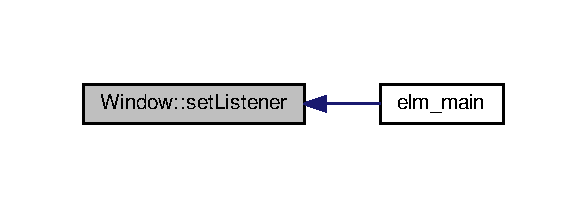
\includegraphics[width=282pt]{class_window_aefe72579d0c1b8308f7c0a5019eecd30_icgraph}
\end{center}
\end{figure}


\hypertarget{class_window_a550a3c5b830d843e9fc3864105eb0127}{\index{Window@{Window}!set\-Rotation@{set\-Rotation}}
\index{set\-Rotation@{set\-Rotation}!Window@{Window}}
\subsubsection[{set\-Rotation}]{\setlength{\rightskip}{0pt plus 5cm}void Window\-::set\-Rotation (
\begin{DoxyParamCaption}
\item[{int}]{rotation}
\end{DoxyParamCaption}
)}}\label{class_window_a550a3c5b830d843e9fc3864105eb0127}
Rotates the window 
\begin{DoxyParams}{Parameters}
{\em rotation} & The rotation of the window, in degrees (0-\/360), \\
\hline
\end{DoxyParams}


Definition at line 147 of file Window.\-cpp.



The documentation for this class was generated from the following files\-:\begin{DoxyCompactItemize}
\item 
\hyperlink{_window_8h}{Window.\-h}\item 
\hyperlink{_window_8cpp}{Window.\-cpp}\end{DoxyCompactItemize}

\hypertarget{class_window_listener}{\section{Window\-Listener Class Reference}
\label{class_window_listener}\index{Window\-Listener@{Window\-Listener}}
}


{\ttfamily \#include $<$Window\-Listener.\-h$>$}



Inheritance diagram for Window\-Listener\-:\nopagebreak
\begin{figure}[H]
\begin{center}
\leavevmode
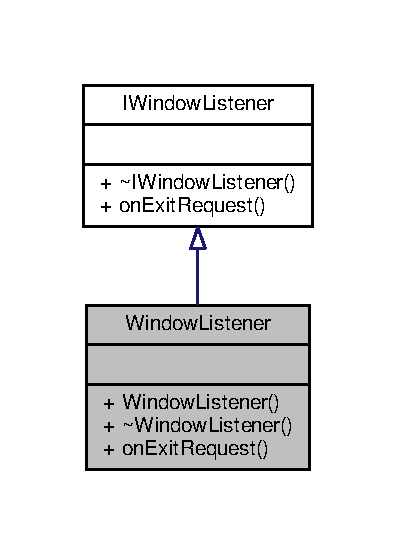
\includegraphics[width=190pt]{class_window_listener__inherit__graph}
\end{center}
\end{figure}


Collaboration diagram for Window\-Listener\-:
\nopagebreak
\begin{figure}[H]
\begin{center}
\leavevmode
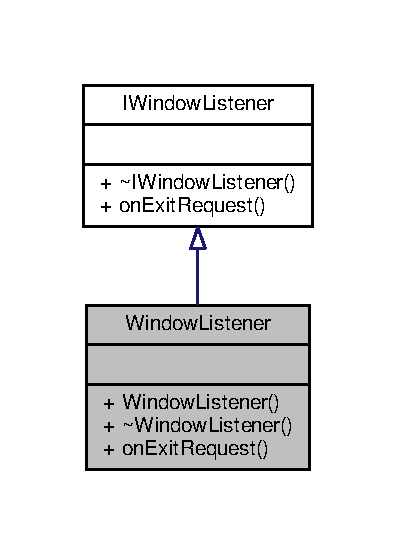
\includegraphics[width=190pt]{class_window_listener__coll__graph}
\end{center}
\end{figure}
\subsection*{Public Member Functions}
\begin{DoxyCompactItemize}
\item 
\hyperlink{class_window_listener_ac7c45d558c826ca380451ecc4276917f}{Window\-Listener} ()
\item 
virtual \hyperlink{class_window_listener_a1578b04817896e39a25640aa7b207dba}{$\sim$\-Window\-Listener} ()
\item 
virtual void \hyperlink{class_window_listener_a2e4f8610046140cc051aa4fa5b609379}{on\-Exit\-Request} (\hyperlink{class_window}{Window} \&win)
\end{DoxyCompactItemize}


\subsection{Detailed Description}


Definition at line 13 of file Window\-Listener.\-h.



\subsection{Constructor \& Destructor Documentation}
\hypertarget{class_window_listener_ac7c45d558c826ca380451ecc4276917f}{\index{Window\-Listener@{Window\-Listener}!Window\-Listener@{Window\-Listener}}
\index{Window\-Listener@{Window\-Listener}!WindowListener@{Window\-Listener}}
\subsubsection[{Window\-Listener}]{\setlength{\rightskip}{0pt plus 5cm}Window\-Listener\-::\-Window\-Listener (
\begin{DoxyParamCaption}
{}
\end{DoxyParamCaption}
)}}\label{class_window_listener_ac7c45d558c826ca380451ecc4276917f}


Definition at line 11 of file Window\-Listener.\-cpp.

\hypertarget{class_window_listener_a1578b04817896e39a25640aa7b207dba}{\index{Window\-Listener@{Window\-Listener}!$\sim$\-Window\-Listener@{$\sim$\-Window\-Listener}}
\index{$\sim$\-Window\-Listener@{$\sim$\-Window\-Listener}!WindowListener@{Window\-Listener}}
\subsubsection[{$\sim$\-Window\-Listener}]{\setlength{\rightskip}{0pt plus 5cm}Window\-Listener\-::$\sim$\-Window\-Listener (
\begin{DoxyParamCaption}
{}
\end{DoxyParamCaption}
)\hspace{0.3cm}{\ttfamily [virtual]}}}\label{class_window_listener_a1578b04817896e39a25640aa7b207dba}


Definition at line 16 of file Window\-Listener.\-cpp.



\subsection{Member Function Documentation}
\hypertarget{class_window_listener_a2e4f8610046140cc051aa4fa5b609379}{\index{Window\-Listener@{Window\-Listener}!on\-Exit\-Request@{on\-Exit\-Request}}
\index{on\-Exit\-Request@{on\-Exit\-Request}!WindowListener@{Window\-Listener}}
\subsubsection[{on\-Exit\-Request}]{\setlength{\rightskip}{0pt plus 5cm}void Window\-Listener\-::on\-Exit\-Request (
\begin{DoxyParamCaption}
\item[{{\bf Window} \&}]{win}
\end{DoxyParamCaption}
)\hspace{0.3cm}{\ttfamily [virtual]}}}\label{class_window_listener_a2e4f8610046140cc051aa4fa5b609379}
Call if user reqest close window 
\begin{DoxyParams}{Parameters}
{\em win} & ref. to \hyperlink{class_window}{Window} object \\
\hline
\end{DoxyParams}


Implements \hyperlink{class_i_window_listener_ae96ae51b613e874865d985e376da01aa}{I\-Window\-Listener}.



Definition at line 20 of file Window\-Listener.\-cpp.



The documentation for this class was generated from the following files\-:\begin{DoxyCompactItemize}
\item 
\hyperlink{_window_listener_8h}{Window\-Listener.\-h}\item 
\hyperlink{_window_listener_8cpp}{Window\-Listener.\-cpp}\end{DoxyCompactItemize}

\chapter{File Documentation}
\hypertarget{_base_view_8cpp}{\section{Base\-View.\-cpp File Reference}
\label{_base_view_8cpp}\index{Base\-View.\-cpp@{Base\-View.\-cpp}}
}


Base View for all view classes.  


{\ttfamily \#include \char`\"{}Base\-View.\-h\char`\"{}}\\*
Include dependency graph for Base\-View.\-cpp\-:\nopagebreak
\begin{figure}[H]
\begin{center}
\leavevmode
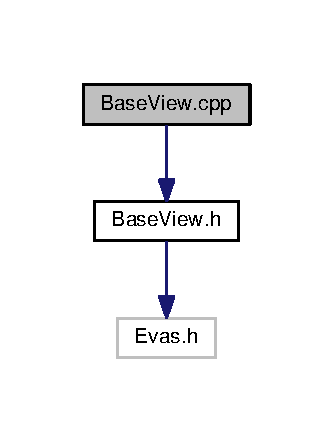
\includegraphics[width=160pt]{_base_view_8cpp__incl}
\end{center}
\end{figure}


\subsection{Detailed Description}
Base View for all view classes. \begin{DoxyAuthor}{Author}
Denis Dolzhenko(\href{mailto:d.dolzhenko@samsung.com}{\tt d.\-dolzhenko@samsung.\-com}) 
\end{DoxyAuthor}


Definition in file \hyperlink{_base_view_8cpp_source}{Base\-View.\-cpp}.


\hypertarget{_base_view_8h}{\section{Base\-View.\-h File Reference}
\label{_base_view_8h}\index{Base\-View.\-h@{Base\-View.\-h}}
}


Base View for all view classes.  


{\ttfamily \#include $<$Evas.\-h$>$}\\*
Include dependency graph for Base\-View.\-h\-:\nopagebreak
\begin{figure}[H]
\begin{center}
\leavevmode
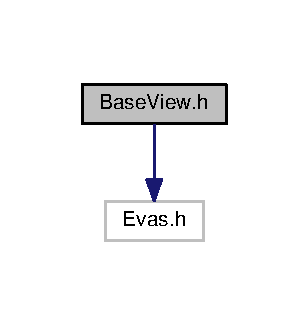
\includegraphics[width=148pt]{_base_view_8h__incl}
\end{center}
\end{figure}
This graph shows which files directly or indirectly include this file\-:\nopagebreak
\begin{figure}[H]
\begin{center}
\leavevmode
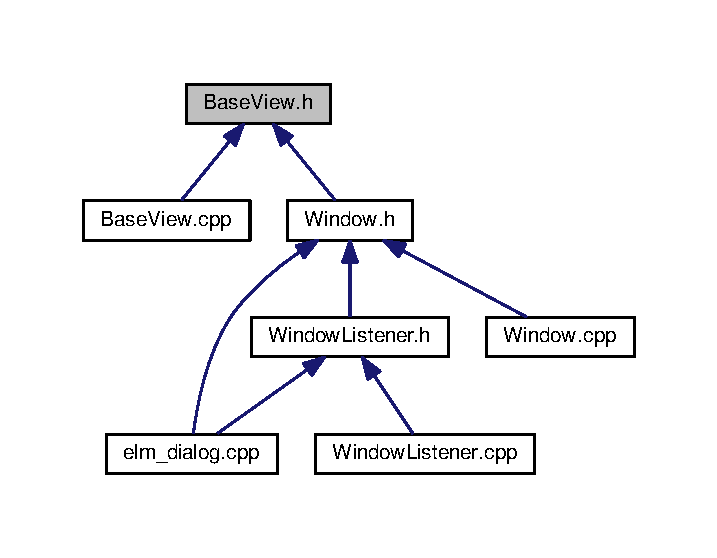
\includegraphics[width=344pt]{_base_view_8h__dep__incl}
\end{center}
\end{figure}
\subsection*{Classes}
\begin{DoxyCompactItemize}
\item 
class \hyperlink{class_base_view}{Base\-View}
\end{DoxyCompactItemize}


\subsection{Detailed Description}
Base View for all view classes. \begin{DoxyAuthor}{Author}
Denis Dolzhenko(\href{mailto:d.dolzhenko@samsung.com}{\tt d.\-dolzhenko@samsung.\-com}) 
\end{DoxyAuthor}


Definition in file \hyperlink{_base_view_8h_source}{Base\-View.\-h}.


\hypertarget{_drawing_content_8cpp}{\section{Drawing\-Content.\-cpp File Reference}
\label{_drawing_content_8cpp}\index{Drawing\-Content.\-cpp@{Drawing\-Content.\-cpp}}
}
{\ttfamily \#include \char`\"{}Drawing\-Content.\-h\char`\"{}}\\*
{\ttfamily \#include \char`\"{}Geometry\-Objects\-Manager.\-h\char`\"{}}\\*
{\ttfamily \#include $<$Elementary.\-h$>$}\\*
{\ttfamily \#include $<$iostream$>$}\\*
{\ttfamily \#include $<$algorithm$>$}\\*
Include dependency graph for Drawing\-Content.\-cpp\-:\nopagebreak
\begin{figure}[H]
\begin{center}
\leavevmode
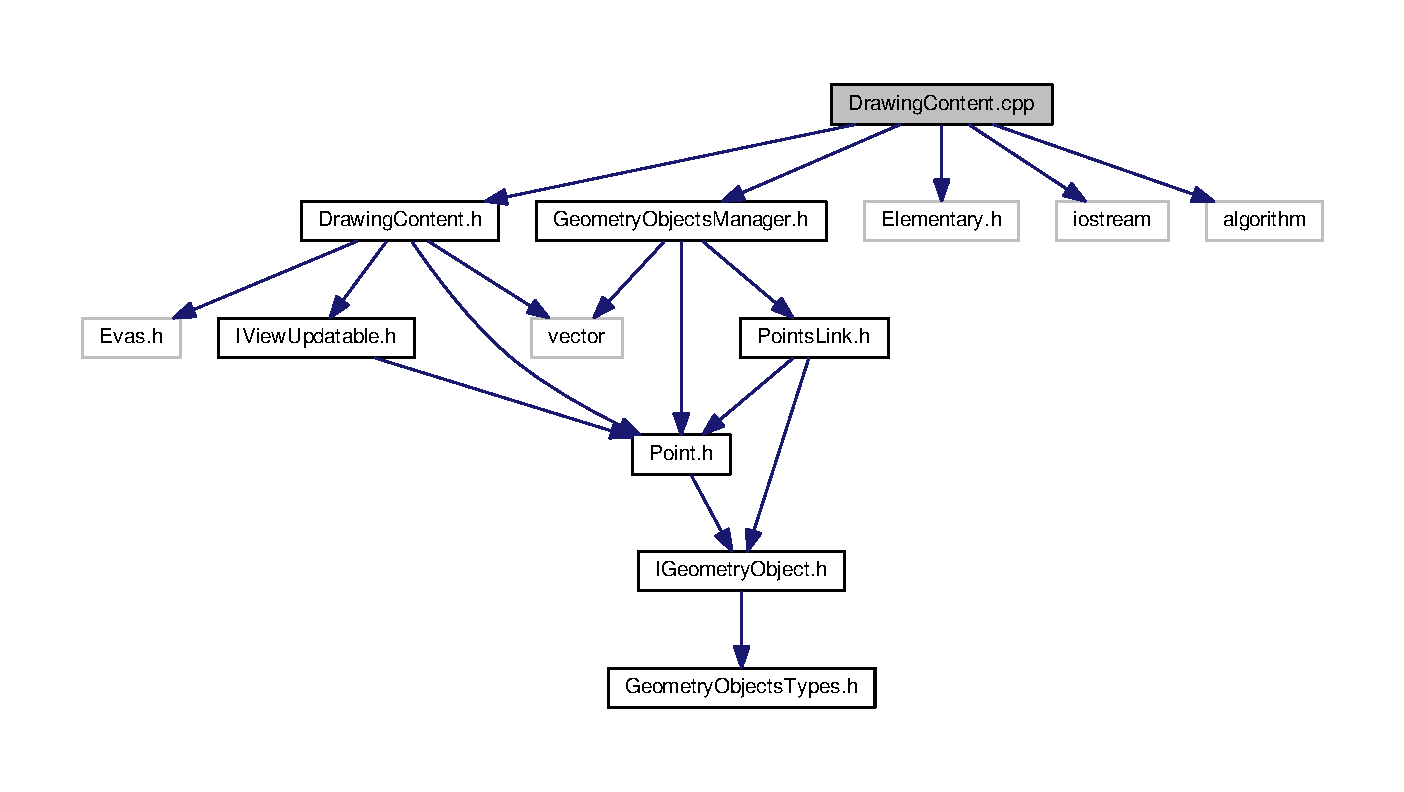
\includegraphics[width=350pt]{_drawing_content_8cpp__incl}
\end{center}
\end{figure}
\subsection*{Macros}
\begin{DoxyCompactItemize}
\item 
\#define \hyperlink{_drawing_content_8cpp_addf4dfb049deddbfe162c8638412af26}{M\-A\-I\-N\-\_\-\-E\-D\-J}~\char`\"{}./main.\-edj\char`\"{}
\item 
\#define \hyperlink{_drawing_content_8cpp_a764171f7d884d73db3eff322dda7ef3a}{S\-E\-A\-R\-C\-H\-I\-N\-G\-\_\-\-P\-O\-I\-N\-T\-\_\-\-R\-A\-D\-I\-U\-S}~20
\end{DoxyCompactItemize}


\subsection{Macro Definition Documentation}
\hypertarget{_drawing_content_8cpp_addf4dfb049deddbfe162c8638412af26}{\index{Drawing\-Content.\-cpp@{Drawing\-Content.\-cpp}!M\-A\-I\-N\-\_\-\-E\-D\-J@{M\-A\-I\-N\-\_\-\-E\-D\-J}}
\index{M\-A\-I\-N\-\_\-\-E\-D\-J@{M\-A\-I\-N\-\_\-\-E\-D\-J}!DrawingContent.cpp@{Drawing\-Content.\-cpp}}
\subsubsection[{M\-A\-I\-N\-\_\-\-E\-D\-J}]{\setlength{\rightskip}{0pt plus 5cm}\#define M\-A\-I\-N\-\_\-\-E\-D\-J~\char`\"{}./main.\-edj\char`\"{}}}\label{_drawing_content_8cpp_addf4dfb049deddbfe162c8638412af26}


Definition at line 15 of file Drawing\-Content.\-cpp.

\hypertarget{_drawing_content_8cpp_a764171f7d884d73db3eff322dda7ef3a}{\index{Drawing\-Content.\-cpp@{Drawing\-Content.\-cpp}!S\-E\-A\-R\-C\-H\-I\-N\-G\-\_\-\-P\-O\-I\-N\-T\-\_\-\-R\-A\-D\-I\-U\-S@{S\-E\-A\-R\-C\-H\-I\-N\-G\-\_\-\-P\-O\-I\-N\-T\-\_\-\-R\-A\-D\-I\-U\-S}}
\index{S\-E\-A\-R\-C\-H\-I\-N\-G\-\_\-\-P\-O\-I\-N\-T\-\_\-\-R\-A\-D\-I\-U\-S@{S\-E\-A\-R\-C\-H\-I\-N\-G\-\_\-\-P\-O\-I\-N\-T\-\_\-\-R\-A\-D\-I\-U\-S}!DrawingContent.cpp@{Drawing\-Content.\-cpp}}
\subsubsection[{S\-E\-A\-R\-C\-H\-I\-N\-G\-\_\-\-P\-O\-I\-N\-T\-\_\-\-R\-A\-D\-I\-U\-S}]{\setlength{\rightskip}{0pt plus 5cm}\#define S\-E\-A\-R\-C\-H\-I\-N\-G\-\_\-\-P\-O\-I\-N\-T\-\_\-\-R\-A\-D\-I\-U\-S~20}}\label{_drawing_content_8cpp_a764171f7d884d73db3eff322dda7ef3a}


Definition at line 17 of file Drawing\-Content.\-cpp.


\hypertarget{_drawing_content_8h}{\section{Drawing\-Content.\-h File Reference}
\label{_drawing_content_8h}\index{Drawing\-Content.\-h@{Drawing\-Content.\-h}}
}
{\ttfamily \#include $<$Evas.\-h$>$}\\*
{\ttfamily \#include $<$vector$>$}\\*
{\ttfamily \#include \char`\"{}I\-View\-Updatable.\-h\char`\"{}}\\*
{\ttfamily \#include \char`\"{}Point.\-h\char`\"{}}\\*
Include dependency graph for Drawing\-Content.\-h\-:\nopagebreak
\begin{figure}[H]
\begin{center}
\leavevmode
\includegraphics[width=350pt]{_drawing_content_8h__incl}
\end{center}
\end{figure}
This graph shows which files directly or indirectly include this file\-:\nopagebreak
\begin{figure}[H]
\begin{center}
\leavevmode
\includegraphics[width=285pt]{_drawing_content_8h__dep__incl}
\end{center}
\end{figure}
\subsection*{Classes}
\begin{DoxyCompactItemize}
\item 
class \hyperlink{class_drawing_content}{Drawing\-Content}
\end{DoxyCompactItemize}

\hypertarget{elm__dialog_8cpp}{\section{elm\-\_\-dialog.\-cpp File Reference}
\label{elm__dialog_8cpp}\index{elm\-\_\-dialog.\-cpp@{elm\-\_\-dialog.\-cpp}}
}
{\ttfamily \#include $<$iostream$>$}\\*
{\ttfamily \#include $<$Elementary.\-h$>$}\\*
{\ttfamily \#include \char`\"{}Window.\-h\char`\"{}}\\*
{\ttfamily \#include \char`\"{}Main\-Content.\-h\char`\"{}}\\*
{\ttfamily \#include \char`\"{}Toolbar\-Content.\-h\char`\"{}}\\*
{\ttfamily \#include \char`\"{}Drawing\-Content.\-h\char`\"{}}\\*
{\ttfamily \#include \char`\"{}Window\-Listener.\-h\char`\"{}}\\*
{\ttfamily \#include \char`\"{}Mouse\-Listener.\-h\char`\"{}}\\*
{\ttfamily \#include \char`\"{}Geometry\-Operation\-Tracking.\-h\char`\"{}}\\*
Include dependency graph for elm\-\_\-dialog.\-cpp\-:\nopagebreak
\begin{figure}[H]
\begin{center}
\leavevmode
\includegraphics[width=350pt]{elm__dialog_8cpp__incl}
\end{center}
\end{figure}
\subsection*{Functions}
\begin{DoxyCompactItemize}
\item 
E\-A\-P\-I\-\_\-\-M\-A\-I\-N int \hyperlink{elm__dialog_8cpp_ad4627be9ebc6a22634b1a2548a3f09d6}{elm\-\_\-main} (int argc, char $\ast$$\ast$argv)
\end{DoxyCompactItemize}


\subsection{Function Documentation}
\hypertarget{elm__dialog_8cpp_ad4627be9ebc6a22634b1a2548a3f09d6}{\index{elm\-\_\-dialog.\-cpp@{elm\-\_\-dialog.\-cpp}!elm\-\_\-main@{elm\-\_\-main}}
\index{elm\-\_\-main@{elm\-\_\-main}!elm_dialog.cpp@{elm\-\_\-dialog.\-cpp}}
\subsubsection[{elm\-\_\-main}]{\setlength{\rightskip}{0pt plus 5cm}E\-A\-P\-I\-\_\-\-M\-A\-I\-N int elm\-\_\-main (
\begin{DoxyParamCaption}
\item[{int}]{argc, }
\item[{char $\ast$$\ast$}]{argv}
\end{DoxyParamCaption}
)}}\label{elm__dialog_8cpp_ad4627be9ebc6a22634b1a2548a3f09d6}


Definition at line 22 of file elm\-\_\-dialog.\-cpp.



Here is the call graph for this function\-:\nopagebreak
\begin{figure}[H]
\begin{center}
\leavevmode
\includegraphics[width=312pt]{elm__dialog_8cpp_ad4627be9ebc6a22634b1a2548a3f09d6_cgraph}
\end{center}
\end{figure}



\hypertarget{_geometry_object_factory_8cpp}{\section{Geometry\-Object\-Factory.\-cpp File Reference}
\label{_geometry_object_factory_8cpp}\index{Geometry\-Object\-Factory.\-cpp@{Geometry\-Object\-Factory.\-cpp}}
}
{\ttfamily \#include \char`\"{}Geometry\-Object\-Factory.\-h\char`\"{}}\\*
{\ttfamily \#include \char`\"{}Point.\-h\char`\"{}}\\*
{\ttfamily \#include \char`\"{}Points\-Link.\-h\char`\"{}}\\*
Include dependency graph for Geometry\-Object\-Factory.\-cpp\-:\nopagebreak
\begin{figure}[H]
\begin{center}
\leavevmode
\includegraphics[width=311pt]{_geometry_object_factory_8cpp__incl}
\end{center}
\end{figure}

\hypertarget{_geometry_object_factory_8h}{\section{Geometry\-Object\-Factory.\-h File Reference}
\label{_geometry_object_factory_8h}\index{Geometry\-Object\-Factory.\-h@{Geometry\-Object\-Factory.\-h}}
}
{\ttfamily \#include \char`\"{}I\-Geometry\-Object.\-h\char`\"{}}\\*
{\ttfamily \#include \char`\"{}Geometry\-Objects\-Types.\-h\char`\"{}}\\*
Include dependency graph for Geometry\-Object\-Factory.\-h\-:\nopagebreak
\begin{figure}[H]
\begin{center}
\leavevmode
\includegraphics[width=232pt]{_geometry_object_factory_8h__incl}
\end{center}
\end{figure}
This graph shows which files directly or indirectly include this file\-:\nopagebreak
\begin{figure}[H]
\begin{center}
\leavevmode
\includegraphics[width=350pt]{_geometry_object_factory_8h__dep__incl}
\end{center}
\end{figure}
\subsection*{Classes}
\begin{DoxyCompactItemize}
\item 
class \hyperlink{class_geometry_object_factory}{Geometry\-Object\-Factory}
\end{DoxyCompactItemize}

\hypertarget{_geometry_objects_manager_8cpp}{\section{Geometry\-Objects\-Manager.\-cpp File Reference}
\label{_geometry_objects_manager_8cpp}\index{Geometry\-Objects\-Manager.\-cpp@{Geometry\-Objects\-Manager.\-cpp}}
}
{\ttfamily \#include \char`\"{}Geometry\-Objects\-Manager.\-h\char`\"{}}\\*
Include dependency graph for Geometry\-Objects\-Manager.\-cpp\-:\nopagebreak
\begin{figure}[H]
\begin{center}
\leavevmode
\includegraphics[width=267pt]{_geometry_objects_manager_8cpp__incl}
\end{center}
\end{figure}
\subsection*{Macros}
\begin{DoxyCompactItemize}
\item 
\#define \hyperlink{_geometry_objects_manager_8cpp_ae6ec26955ffd41b6ecd85ae5f54c6c1f}{U\-N\-\_\-\-T\-R\-A\-C\-K\-I\-N\-G\-\_\-\-P\-O\-I\-N\-T\-\_\-\-R\-A\-D\-I\-U\-S}~40
\end{DoxyCompactItemize}


\subsection{Macro Definition Documentation}
\hypertarget{_geometry_objects_manager_8cpp_ae6ec26955ffd41b6ecd85ae5f54c6c1f}{\index{Geometry\-Objects\-Manager.\-cpp@{Geometry\-Objects\-Manager.\-cpp}!U\-N\-\_\-\-T\-R\-A\-C\-K\-I\-N\-G\-\_\-\-P\-O\-I\-N\-T\-\_\-\-R\-A\-D\-I\-U\-S@{U\-N\-\_\-\-T\-R\-A\-C\-K\-I\-N\-G\-\_\-\-P\-O\-I\-N\-T\-\_\-\-R\-A\-D\-I\-U\-S}}
\index{U\-N\-\_\-\-T\-R\-A\-C\-K\-I\-N\-G\-\_\-\-P\-O\-I\-N\-T\-\_\-\-R\-A\-D\-I\-U\-S@{U\-N\-\_\-\-T\-R\-A\-C\-K\-I\-N\-G\-\_\-\-P\-O\-I\-N\-T\-\_\-\-R\-A\-D\-I\-U\-S}!GeometryObjectsManager.cpp@{Geometry\-Objects\-Manager.\-cpp}}
\subsubsection[{U\-N\-\_\-\-T\-R\-A\-C\-K\-I\-N\-G\-\_\-\-P\-O\-I\-N\-T\-\_\-\-R\-A\-D\-I\-U\-S}]{\setlength{\rightskip}{0pt plus 5cm}\#define U\-N\-\_\-\-T\-R\-A\-C\-K\-I\-N\-G\-\_\-\-P\-O\-I\-N\-T\-\_\-\-R\-A\-D\-I\-U\-S~40}}\label{_geometry_objects_manager_8cpp_ae6ec26955ffd41b6ecd85ae5f54c6c1f}


Definition at line 10 of file Geometry\-Objects\-Manager.\-cpp.


\hypertarget{_geometry_objects_manager_8h}{\section{Geometry\-Objects\-Manager.\-h File Reference}
\label{_geometry_objects_manager_8h}\index{Geometry\-Objects\-Manager.\-h@{Geometry\-Objects\-Manager.\-h}}
}
{\ttfamily \#include \char`\"{}Point.\-h\char`\"{}}\\*
{\ttfamily \#include \char`\"{}Points\-Link.\-h\char`\"{}}\\*
{\ttfamily \#include $<$vector$>$}\\*
Include dependency graph for Geometry\-Objects\-Manager.\-h\-:\nopagebreak
\begin{figure}[H]
\begin{center}
\leavevmode
\includegraphics[width=267pt]{_geometry_objects_manager_8h__incl}
\end{center}
\end{figure}
This graph shows which files directly or indirectly include this file\-:\nopagebreak
\begin{figure}[H]
\begin{center}
\leavevmode
\includegraphics[width=350pt]{_geometry_objects_manager_8h__dep__incl}
\end{center}
\end{figure}
\subsection*{Classes}
\begin{DoxyCompactItemize}
\item 
class \hyperlink{class_geometry_objects_manager}{Geometry\-Objects\-Manager}
\end{DoxyCompactItemize}

\hypertarget{_geometry_objects_types_8h}{\section{Geometry\-Objects\-Types.\-h File Reference}
\label{_geometry_objects_types_8h}\index{Geometry\-Objects\-Types.\-h@{Geometry\-Objects\-Types.\-h}}
}
This graph shows which files directly or indirectly include this file\-:\nopagebreak
\begin{figure}[H]
\begin{center}
\leavevmode
\includegraphics[width=350pt]{_geometry_objects_types_8h__dep__incl}
\end{center}
\end{figure}
\subsection*{Enumerations}
\begin{DoxyCompactItemize}
\item 
enum \hyperlink{_geometry_objects_types_8h_adea8b8c3a289ca1fc1450d9424dcd33d}{Geometry\-Objects\-Types} \{ \hyperlink{_geometry_objects_types_8h_adea8b8c3a289ca1fc1450d9424dcd33daee15602406420a789151d4a4b3b3a1fd}{G\-E\-O\-M\-E\-T\-R\-Y\-O\-B\-J\-E\-C\-T\-\_\-\-P\-O\-I\-N\-T}, 
\hyperlink{_geometry_objects_types_8h_adea8b8c3a289ca1fc1450d9424dcd33dac31e310bb4971f1df89c251143ebd2d4}{G\-E\-O\-M\-E\-T\-R\-Y\-O\-B\-J\-E\-C\-T\-\_\-\-L\-I\-N\-K}
 \}
\end{DoxyCompactItemize}


\subsection{Enumeration Type Documentation}
\hypertarget{_geometry_objects_types_8h_adea8b8c3a289ca1fc1450d9424dcd33d}{\index{Geometry\-Objects\-Types.\-h@{Geometry\-Objects\-Types.\-h}!Geometry\-Objects\-Types@{Geometry\-Objects\-Types}}
\index{Geometry\-Objects\-Types@{Geometry\-Objects\-Types}!GeometryObjectsTypes.h@{Geometry\-Objects\-Types.\-h}}
\subsubsection[{Geometry\-Objects\-Types}]{\setlength{\rightskip}{0pt plus 5cm}enum {\bf Geometry\-Objects\-Types}}}\label{_geometry_objects_types_8h_adea8b8c3a289ca1fc1450d9424dcd33d}
\begin{Desc}
\item[Enumerator]\par
\begin{description}
\index{G\-E\-O\-M\-E\-T\-R\-Y\-O\-B\-J\-E\-C\-T\-\_\-\-P\-O\-I\-N\-T@{G\-E\-O\-M\-E\-T\-R\-Y\-O\-B\-J\-E\-C\-T\-\_\-\-P\-O\-I\-N\-T}!Geometry\-Objects\-Types.\-h@{Geometry\-Objects\-Types.\-h}}\index{Geometry\-Objects\-Types.\-h@{Geometry\-Objects\-Types.\-h}!G\-E\-O\-M\-E\-T\-R\-Y\-O\-B\-J\-E\-C\-T\-\_\-\-P\-O\-I\-N\-T@{G\-E\-O\-M\-E\-T\-R\-Y\-O\-B\-J\-E\-C\-T\-\_\-\-P\-O\-I\-N\-T}}\item[{\em 
\hypertarget{_geometry_objects_types_8h_adea8b8c3a289ca1fc1450d9424dcd33daee15602406420a789151d4a4b3b3a1fd}{G\-E\-O\-M\-E\-T\-R\-Y\-O\-B\-J\-E\-C\-T\-\_\-\-P\-O\-I\-N\-T}\label{_geometry_objects_types_8h_adea8b8c3a289ca1fc1450d9424dcd33daee15602406420a789151d4a4b3b3a1fd}
}]\index{G\-E\-O\-M\-E\-T\-R\-Y\-O\-B\-J\-E\-C\-T\-\_\-\-L\-I\-N\-K@{G\-E\-O\-M\-E\-T\-R\-Y\-O\-B\-J\-E\-C\-T\-\_\-\-L\-I\-N\-K}!Geometry\-Objects\-Types.\-h@{Geometry\-Objects\-Types.\-h}}\index{Geometry\-Objects\-Types.\-h@{Geometry\-Objects\-Types.\-h}!G\-E\-O\-M\-E\-T\-R\-Y\-O\-B\-J\-E\-C\-T\-\_\-\-L\-I\-N\-K@{G\-E\-O\-M\-E\-T\-R\-Y\-O\-B\-J\-E\-C\-T\-\_\-\-L\-I\-N\-K}}\item[{\em 
\hypertarget{_geometry_objects_types_8h_adea8b8c3a289ca1fc1450d9424dcd33dac31e310bb4971f1df89c251143ebd2d4}{G\-E\-O\-M\-E\-T\-R\-Y\-O\-B\-J\-E\-C\-T\-\_\-\-L\-I\-N\-K}\label{_geometry_objects_types_8h_adea8b8c3a289ca1fc1450d9424dcd33dac31e310bb4971f1df89c251143ebd2d4}
}]\end{description}
\end{Desc}


Definition at line 12 of file Geometry\-Objects\-Types.\-h.


\hypertarget{_geometry_operation_tracking_8cpp}{\section{Geometry\-Operation\-Tracking.\-cpp File Reference}
\label{_geometry_operation_tracking_8cpp}\index{Geometry\-Operation\-Tracking.\-cpp@{Geometry\-Operation\-Tracking.\-cpp}}
}
{\ttfamily \#include \char`\"{}Geometry\-Operation\-Tracking.\-h\char`\"{}}\\*
{\ttfamily \#include \char`\"{}Geometry\-Objects\-Manager.\-h\char`\"{}}\\*
{\ttfamily \#include \char`\"{}Geometry\-Object\-Factory.\-h\char`\"{}}\\*
Include dependency graph for Geometry\-Operation\-Tracking.\-cpp\-:\nopagebreak
\begin{figure}[H]
\begin{center}
\leavevmode
\includegraphics[width=350pt]{_geometry_operation_tracking_8cpp__incl}
\end{center}
\end{figure}

\hypertarget{_geometry_operation_tracking_8h}{\section{Geometry\-Operation\-Tracking.\-h File Reference}
\label{_geometry_operation_tracking_8h}\index{Geometry\-Operation\-Tracking.\-h@{Geometry\-Operation\-Tracking.\-h}}
}
{\ttfamily \#include \char`\"{}I\-Geometry\-Object\-Tracker.\-h\char`\"{}}\\*
{\ttfamily \#include \char`\"{}Object\-Operation\-Status.\-h\char`\"{}}\\*
{\ttfamily \#include \char`\"{}I\-View\-Updatable.\-h\char`\"{}}\\*
{\ttfamily \#include \char`\"{}Point.\-h\char`\"{}}\\*
{\ttfamily \#include $<$vector$>$}\\*
Include dependency graph for Geometry\-Operation\-Tracking.\-h\-:\nopagebreak
\begin{figure}[H]
\begin{center}
\leavevmode
\includegraphics[width=350pt]{_geometry_operation_tracking_8h__incl}
\end{center}
\end{figure}
This graph shows which files directly or indirectly include this file\-:\nopagebreak
\begin{figure}[H]
\begin{center}
\leavevmode
\includegraphics[width=337pt]{_geometry_operation_tracking_8h__dep__incl}
\end{center}
\end{figure}
\subsection*{Classes}
\begin{DoxyCompactItemize}
\item 
class \hyperlink{class_geometry_operation_tracking}{Geometry\-Operation\-Tracking}
\end{DoxyCompactItemize}

\hypertarget{_i_geometry_object_8h}{\section{I\-Geometry\-Object.\-h File Reference}
\label{_i_geometry_object_8h}\index{I\-Geometry\-Object.\-h@{I\-Geometry\-Object.\-h}}
}
{\ttfamily \#include \char`\"{}Geometry\-Objects\-Types.\-h\char`\"{}}\\*
Include dependency graph for I\-Geometry\-Object.\-h\-:\nopagebreak
\begin{figure}[H]
\begin{center}
\leavevmode
\includegraphics[width=208pt]{_i_geometry_object_8h__incl}
\end{center}
\end{figure}
This graph shows which files directly or indirectly include this file\-:\nopagebreak
\begin{figure}[H]
\begin{center}
\leavevmode
\includegraphics[width=350pt]{_i_geometry_object_8h__dep__incl}
\end{center}
\end{figure}
\subsection*{Classes}
\begin{DoxyCompactItemize}
\item 
class \hyperlink{class_i_geometry_object}{I\-Geometry\-Object}
\end{DoxyCompactItemize}

\hypertarget{_i_geometry_object_tracker_8h}{\section{I\-Geometry\-Object\-Tracker.\-h File Reference}
\label{_i_geometry_object_tracker_8h}\index{I\-Geometry\-Object\-Tracker.\-h@{I\-Geometry\-Object\-Tracker.\-h}}
}
This graph shows which files directly or indirectly include this file\-:\nopagebreak
\begin{figure}[H]
\begin{center}
\leavevmode
\includegraphics[width=350pt]{_i_geometry_object_tracker_8h__dep__incl}
\end{center}
\end{figure}
\subsection*{Classes}
\begin{DoxyCompactItemize}
\item 
class \hyperlink{class_i_geometry_object_tracker}{I\-Geometry\-Object\-Tracker}
\end{DoxyCompactItemize}

\hypertarget{_i_view_updatable_8h}{\section{I\-View\-Updatable.\-h File Reference}
\label{_i_view_updatable_8h}\index{I\-View\-Updatable.\-h@{I\-View\-Updatable.\-h}}
}
{\ttfamily \#include \char`\"{}Point.\-h\char`\"{}}\\*
Include dependency graph for I\-View\-Updatable.\-h\-:\nopagebreak
\begin{figure}[H]
\begin{center}
\leavevmode
\includegraphics[width=208pt]{_i_view_updatable_8h__incl}
\end{center}
\end{figure}
This graph shows which files directly or indirectly include this file\-:\nopagebreak
\begin{figure}[H]
\begin{center}
\leavevmode
\includegraphics[width=350pt]{_i_view_updatable_8h__dep__incl}
\end{center}
\end{figure}
\subsection*{Classes}
\begin{DoxyCompactItemize}
\item 
class \hyperlink{class_i_view_updatable}{I\-View\-Updatable}
\end{DoxyCompactItemize}

\hypertarget{_main_content_8cpp}{\section{Main\-Content.\-cpp File Reference}
\label{_main_content_8cpp}\index{Main\-Content.\-cpp@{Main\-Content.\-cpp}}
}
{\ttfamily \#include \char`\"{}Main\-Content.\-h\char`\"{}}\\*
{\ttfamily \#include $<$Elementary.\-h$>$}\\*
{\ttfamily \#include $<$Evas\-\_\-\-Engine\-\_\-\-Buffer.\-h$>$}\\*
{\ttfamily \#include $<$iostream$>$}\\*
Include dependency graph for Main\-Content.\-cpp\-:\nopagebreak
\begin{figure}[H]
\begin{center}
\leavevmode
\includegraphics[width=350pt]{_main_content_8cpp__incl}
\end{center}
\end{figure}
\subsection*{Macros}
\begin{DoxyCompactItemize}
\item 
\#define \hyperlink{_main_content_8cpp_addf4dfb049deddbfe162c8638412af26}{M\-A\-I\-N\-\_\-\-E\-D\-J}~\char`\"{}./main.\-edj\char`\"{}
\end{DoxyCompactItemize}


\subsection{Macro Definition Documentation}
\hypertarget{_main_content_8cpp_addf4dfb049deddbfe162c8638412af26}{\index{Main\-Content.\-cpp@{Main\-Content.\-cpp}!M\-A\-I\-N\-\_\-\-E\-D\-J@{M\-A\-I\-N\-\_\-\-E\-D\-J}}
\index{M\-A\-I\-N\-\_\-\-E\-D\-J@{M\-A\-I\-N\-\_\-\-E\-D\-J}!MainContent.cpp@{Main\-Content.\-cpp}}
\subsubsection[{M\-A\-I\-N\-\_\-\-E\-D\-J}]{\setlength{\rightskip}{0pt plus 5cm}\#define M\-A\-I\-N\-\_\-\-E\-D\-J~\char`\"{}./main.\-edj\char`\"{}}}\label{_main_content_8cpp_addf4dfb049deddbfe162c8638412af26}


Definition at line 16 of file Main\-Content.\-cpp.


\hypertarget{_main_content_8h}{\section{Main\-Content.\-h File Reference}
\label{_main_content_8h}\index{Main\-Content.\-h@{Main\-Content.\-h}}
}
{\ttfamily \#include $<$Evas.\-h$>$}\\*
Include dependency graph for Main\-Content.\-h\-:\nopagebreak
\begin{figure}[H]
\begin{center}
\leavevmode
\includegraphics[width=160pt]{_main_content_8h__incl}
\end{center}
\end{figure}
This graph shows which files directly or indirectly include this file\-:\nopagebreak
\begin{figure}[H]
\begin{center}
\leavevmode
\includegraphics[width=271pt]{_main_content_8h__dep__incl}
\end{center}
\end{figure}
\subsection*{Classes}
\begin{DoxyCompactItemize}
\item 
class \hyperlink{class_main_content}{Main\-Content}
\end{DoxyCompactItemize}

\hypertarget{_mouse_listener_8cpp}{\section{Mouse\-Listener.\-cpp File Reference}
\label{_mouse_listener_8cpp}\index{Mouse\-Listener.\-cpp@{Mouse\-Listener.\-cpp}}
}
{\ttfamily \#include \char`\"{}Mouse\-Listener.\-h\char`\"{}}\\*
{\ttfamily \#include $<$iostream$>$}\\*
Include dependency graph for Mouse\-Listener.\-cpp\-:\nopagebreak
\begin{figure}[H]
\begin{center}
\leavevmode
\includegraphics[width=277pt]{_mouse_listener_8cpp__incl}
\end{center}
\end{figure}

\hypertarget{_mouse_listener_8h}{\section{Mouse\-Listener.\-h File Reference}
\label{_mouse_listener_8h}\index{Mouse\-Listener.\-h@{Mouse\-Listener.\-h}}
}
{\ttfamily \#include $<$Evas.\-h$>$}\\*
{\ttfamily \#include \char`\"{}I\-Geometry\-Object\-Tracker.\-h\char`\"{}}\\*
Include dependency graph for Mouse\-Listener.\-h\-:\nopagebreak
\begin{figure}[H]
\begin{center}
\leavevmode
\includegraphics[width=277pt]{_mouse_listener_8h__incl}
\end{center}
\end{figure}
This graph shows which files directly or indirectly include this file\-:\nopagebreak
\begin{figure}[H]
\begin{center}
\leavevmode
\includegraphics[width=279pt]{_mouse_listener_8h__dep__incl}
\end{center}
\end{figure}
\subsection*{Classes}
\begin{DoxyCompactItemize}
\item 
class \hyperlink{class_mouse_listener}{Mouse\-Listener}
\end{DoxyCompactItemize}

\hypertarget{_object_operation_status_8h}{\section{Object\-Operation\-Status.\-h File Reference}
\label{_object_operation_status_8h}\index{Object\-Operation\-Status.\-h@{Object\-Operation\-Status.\-h}}
}
This graph shows which files directly or indirectly include this file\-:\nopagebreak
\begin{figure}[H]
\begin{center}
\leavevmode
\includegraphics[width=337pt]{_object_operation_status_8h__dep__incl}
\end{center}
\end{figure}
\subsection*{Enumerations}
\begin{DoxyCompactItemize}
\item 
enum \hyperlink{_object_operation_status_8h_a421f61b6f60de2a3da448b2790134f99}{Object\-State} \{ \\*
\hyperlink{_object_operation_status_8h_a421f61b6f60de2a3da448b2790134f99a4935756997f731df406a527a22af531c}{O\-B\-J\-E\-C\-T\-\_\-\-N\-O\-N\-E}, 
\hyperlink{_object_operation_status_8h_a421f61b6f60de2a3da448b2790134f99a4a2cc75d420a142cf094998daf1d721e}{O\-B\-J\-E\-C\-T\-\_\-\-P\-O\-I\-N\-T\-\_\-\-C\-R\-E\-A\-T\-I\-N\-G}, 
\hyperlink{_object_operation_status_8h_a421f61b6f60de2a3da448b2790134f99adbc6857fc6e8d292c96f8fceef32f17b}{O\-B\-J\-E\-C\-T\-\_\-\-P\-O\-I\-N\-T\-\_\-\-C\-R\-E\-A\-T\-E\-D}, 
\hyperlink{_object_operation_status_8h_a421f61b6f60de2a3da448b2790134f99a31bb8887aebac8971a01995e6fd6ea41}{O\-B\-J\-E\-C\-T\-\_\-\-L\-I\-N\-K\-\_\-\-C\-R\-E\-A\-T\-I\-N\-G}, 
\\*
\hyperlink{_object_operation_status_8h_a421f61b6f60de2a3da448b2790134f99a4b253b5b55296a54d5fc7441b6aba1b3}{O\-B\-J\-E\-C\-T\-\_\-\-L\-I\-N\-K\-\_\-\-C\-R\-E\-A\-T\-E\-D}
 \}
\end{DoxyCompactItemize}


\subsection{Enumeration Type Documentation}
\hypertarget{_object_operation_status_8h_a421f61b6f60de2a3da448b2790134f99}{\index{Object\-Operation\-Status.\-h@{Object\-Operation\-Status.\-h}!Object\-State@{Object\-State}}
\index{Object\-State@{Object\-State}!ObjectOperationStatus.h@{Object\-Operation\-Status.\-h}}
\subsubsection[{Object\-State}]{\setlength{\rightskip}{0pt plus 5cm}enum {\bf Object\-State}}}\label{_object_operation_status_8h_a421f61b6f60de2a3da448b2790134f99}
\begin{Desc}
\item[Enumerator]\par
\begin{description}
\index{O\-B\-J\-E\-C\-T\-\_\-\-N\-O\-N\-E@{O\-B\-J\-E\-C\-T\-\_\-\-N\-O\-N\-E}!Object\-Operation\-Status.\-h@{Object\-Operation\-Status.\-h}}\index{Object\-Operation\-Status.\-h@{Object\-Operation\-Status.\-h}!O\-B\-J\-E\-C\-T\-\_\-\-N\-O\-N\-E@{O\-B\-J\-E\-C\-T\-\_\-\-N\-O\-N\-E}}\item[{\em 
\hypertarget{_object_operation_status_8h_a421f61b6f60de2a3da448b2790134f99a4935756997f731df406a527a22af531c}{O\-B\-J\-E\-C\-T\-\_\-\-N\-O\-N\-E}\label{_object_operation_status_8h_a421f61b6f60de2a3da448b2790134f99a4935756997f731df406a527a22af531c}
}]\index{O\-B\-J\-E\-C\-T\-\_\-\-P\-O\-I\-N\-T\-\_\-\-C\-R\-E\-A\-T\-I\-N\-G@{O\-B\-J\-E\-C\-T\-\_\-\-P\-O\-I\-N\-T\-\_\-\-C\-R\-E\-A\-T\-I\-N\-G}!Object\-Operation\-Status.\-h@{Object\-Operation\-Status.\-h}}\index{Object\-Operation\-Status.\-h@{Object\-Operation\-Status.\-h}!O\-B\-J\-E\-C\-T\-\_\-\-P\-O\-I\-N\-T\-\_\-\-C\-R\-E\-A\-T\-I\-N\-G@{O\-B\-J\-E\-C\-T\-\_\-\-P\-O\-I\-N\-T\-\_\-\-C\-R\-E\-A\-T\-I\-N\-G}}\item[{\em 
\hypertarget{_object_operation_status_8h_a421f61b6f60de2a3da448b2790134f99a4a2cc75d420a142cf094998daf1d721e}{O\-B\-J\-E\-C\-T\-\_\-\-P\-O\-I\-N\-T\-\_\-\-C\-R\-E\-A\-T\-I\-N\-G}\label{_object_operation_status_8h_a421f61b6f60de2a3da448b2790134f99a4a2cc75d420a142cf094998daf1d721e}
}]\index{O\-B\-J\-E\-C\-T\-\_\-\-P\-O\-I\-N\-T\-\_\-\-C\-R\-E\-A\-T\-E\-D@{O\-B\-J\-E\-C\-T\-\_\-\-P\-O\-I\-N\-T\-\_\-\-C\-R\-E\-A\-T\-E\-D}!Object\-Operation\-Status.\-h@{Object\-Operation\-Status.\-h}}\index{Object\-Operation\-Status.\-h@{Object\-Operation\-Status.\-h}!O\-B\-J\-E\-C\-T\-\_\-\-P\-O\-I\-N\-T\-\_\-\-C\-R\-E\-A\-T\-E\-D@{O\-B\-J\-E\-C\-T\-\_\-\-P\-O\-I\-N\-T\-\_\-\-C\-R\-E\-A\-T\-E\-D}}\item[{\em 
\hypertarget{_object_operation_status_8h_a421f61b6f60de2a3da448b2790134f99adbc6857fc6e8d292c96f8fceef32f17b}{O\-B\-J\-E\-C\-T\-\_\-\-P\-O\-I\-N\-T\-\_\-\-C\-R\-E\-A\-T\-E\-D}\label{_object_operation_status_8h_a421f61b6f60de2a3da448b2790134f99adbc6857fc6e8d292c96f8fceef32f17b}
}]\index{O\-B\-J\-E\-C\-T\-\_\-\-L\-I\-N\-K\-\_\-\-C\-R\-E\-A\-T\-I\-N\-G@{O\-B\-J\-E\-C\-T\-\_\-\-L\-I\-N\-K\-\_\-\-C\-R\-E\-A\-T\-I\-N\-G}!Object\-Operation\-Status.\-h@{Object\-Operation\-Status.\-h}}\index{Object\-Operation\-Status.\-h@{Object\-Operation\-Status.\-h}!O\-B\-J\-E\-C\-T\-\_\-\-L\-I\-N\-K\-\_\-\-C\-R\-E\-A\-T\-I\-N\-G@{O\-B\-J\-E\-C\-T\-\_\-\-L\-I\-N\-K\-\_\-\-C\-R\-E\-A\-T\-I\-N\-G}}\item[{\em 
\hypertarget{_object_operation_status_8h_a421f61b6f60de2a3da448b2790134f99a31bb8887aebac8971a01995e6fd6ea41}{O\-B\-J\-E\-C\-T\-\_\-\-L\-I\-N\-K\-\_\-\-C\-R\-E\-A\-T\-I\-N\-G}\label{_object_operation_status_8h_a421f61b6f60de2a3da448b2790134f99a31bb8887aebac8971a01995e6fd6ea41}
}]\index{O\-B\-J\-E\-C\-T\-\_\-\-L\-I\-N\-K\-\_\-\-C\-R\-E\-A\-T\-E\-D@{O\-B\-J\-E\-C\-T\-\_\-\-L\-I\-N\-K\-\_\-\-C\-R\-E\-A\-T\-E\-D}!Object\-Operation\-Status.\-h@{Object\-Operation\-Status.\-h}}\index{Object\-Operation\-Status.\-h@{Object\-Operation\-Status.\-h}!O\-B\-J\-E\-C\-T\-\_\-\-L\-I\-N\-K\-\_\-\-C\-R\-E\-A\-T\-E\-D@{O\-B\-J\-E\-C\-T\-\_\-\-L\-I\-N\-K\-\_\-\-C\-R\-E\-A\-T\-E\-D}}\item[{\em 
\hypertarget{_object_operation_status_8h_a421f61b6f60de2a3da448b2790134f99a4b253b5b55296a54d5fc7441b6aba1b3}{O\-B\-J\-E\-C\-T\-\_\-\-L\-I\-N\-K\-\_\-\-C\-R\-E\-A\-T\-E\-D}\label{_object_operation_status_8h_a421f61b6f60de2a3da448b2790134f99a4b253b5b55296a54d5fc7441b6aba1b3}
}]\end{description}
\end{Desc}


Definition at line 12 of file Object\-Operation\-Status.\-h.


\hypertarget{_point_8cpp}{\section{Point.\-cpp File Reference}
\label{_point_8cpp}\index{Point.\-cpp@{Point.\-cpp}}
}
{\ttfamily \#include \char`\"{}Point.\-h\char`\"{}}\\*
Include dependency graph for Point.\-cpp\-:\nopagebreak
\begin{figure}[H]
\begin{center}
\leavevmode
\includegraphics[width=208pt]{_point_8cpp__incl}
\end{center}
\end{figure}

\hypertarget{_point_8h}{\section{Point.\-h File Reference}
\label{_point_8h}\index{Point.\-h@{Point.\-h}}
}
{\ttfamily \#include \char`\"{}I\-Geometry\-Object.\-h\char`\"{}}\\*
Include dependency graph for Point.\-h\-:\nopagebreak
\begin{figure}[H]
\begin{center}
\leavevmode
\includegraphics[width=208pt]{_point_8h__incl}
\end{center}
\end{figure}
This graph shows which files directly or indirectly include this file\-:\nopagebreak
\begin{figure}[H]
\begin{center}
\leavevmode
\includegraphics[width=350pt]{_point_8h__dep__incl}
\end{center}
\end{figure}
\subsection*{Classes}
\begin{DoxyCompactItemize}
\item 
class \hyperlink{class_point}{Point}
\end{DoxyCompactItemize}

\hypertarget{_points_link_8cpp}{\section{Points\-Link.\-cpp File Reference}
\label{_points_link_8cpp}\index{Points\-Link.\-cpp@{Points\-Link.\-cpp}}
}
{\ttfamily \#include \char`\"{}Points\-Link.\-h\char`\"{}}\\*
Include dependency graph for Points\-Link.\-cpp\-:\nopagebreak
\begin{figure}[H]
\begin{center}
\leavevmode
\includegraphics[width=208pt]{_points_link_8cpp__incl}
\end{center}
\end{figure}

\hypertarget{_points_link_8h}{\section{Points\-Link.\-h File Reference}
\label{_points_link_8h}\index{Points\-Link.\-h@{Points\-Link.\-h}}
}
{\ttfamily \#include \char`\"{}Point.\-h\char`\"{}}\\*
{\ttfamily \#include \char`\"{}I\-Geometry\-Object.\-h\char`\"{}}\\*
Include dependency graph for Points\-Link.\-h\-:\nopagebreak
\begin{figure}[H]
\begin{center}
\leavevmode
\includegraphics[width=208pt]{_points_link_8h__incl}
\end{center}
\end{figure}
This graph shows which files directly or indirectly include this file\-:\nopagebreak
\begin{figure}[H]
\begin{center}
\leavevmode
\includegraphics[width=350pt]{_points_link_8h__dep__incl}
\end{center}
\end{figure}
\subsection*{Classes}
\begin{DoxyCompactItemize}
\item 
class \hyperlink{class_points_link}{Points\-Link}
\end{DoxyCompactItemize}

\hypertarget{_toolbar_content_8cpp}{\section{Toolbar\-Content.\-cpp File Reference}
\label{_toolbar_content_8cpp}\index{Toolbar\-Content.\-cpp@{Toolbar\-Content.\-cpp}}
}
{\ttfamily \#include \char`\"{}Toolbar\-Content.\-h\char`\"{}}\\*
{\ttfamily \#include $<$Elementary.\-h$>$}\\*
{\ttfamily \#include $<$iostream$>$}\\*
Include dependency graph for Toolbar\-Content.\-cpp\-:\nopagebreak
\begin{figure}[H]
\begin{center}
\leavevmode
\includegraphics[width=336pt]{_toolbar_content_8cpp__incl}
\end{center}
\end{figure}
\subsection*{Macros}
\begin{DoxyCompactItemize}
\item 
\#define \hyperlink{_toolbar_content_8cpp_addf4dfb049deddbfe162c8638412af26}{M\-A\-I\-N\-\_\-\-E\-D\-J}~\char`\"{}./main.\-edj\char`\"{}
\end{DoxyCompactItemize}
\subsection*{Functions}
\begin{DoxyCompactItemize}
\item 
void \hyperlink{_toolbar_content_8cpp_a4841c36e278db4339e33aa122c19bd72}{on\-\_\-clicked} (void $\ast$data, Evas\-\_\-\-Object $\ast$obj, void $\ast$event\-\_\-info)
\end{DoxyCompactItemize}


\subsection{Macro Definition Documentation}
\hypertarget{_toolbar_content_8cpp_addf4dfb049deddbfe162c8638412af26}{\index{Toolbar\-Content.\-cpp@{Toolbar\-Content.\-cpp}!M\-A\-I\-N\-\_\-\-E\-D\-J@{M\-A\-I\-N\-\_\-\-E\-D\-J}}
\index{M\-A\-I\-N\-\_\-\-E\-D\-J@{M\-A\-I\-N\-\_\-\-E\-D\-J}!ToolbarContent.cpp@{Toolbar\-Content.\-cpp}}
\subsubsection[{M\-A\-I\-N\-\_\-\-E\-D\-J}]{\setlength{\rightskip}{0pt plus 5cm}\#define M\-A\-I\-N\-\_\-\-E\-D\-J~\char`\"{}./main.\-edj\char`\"{}}}\label{_toolbar_content_8cpp_addf4dfb049deddbfe162c8638412af26}


Definition at line 14 of file Toolbar\-Content.\-cpp.



\subsection{Function Documentation}
\hypertarget{_toolbar_content_8cpp_a4841c36e278db4339e33aa122c19bd72}{\index{Toolbar\-Content.\-cpp@{Toolbar\-Content.\-cpp}!on\-\_\-clicked@{on\-\_\-clicked}}
\index{on\-\_\-clicked@{on\-\_\-clicked}!ToolbarContent.cpp@{Toolbar\-Content.\-cpp}}
\subsubsection[{on\-\_\-clicked}]{\setlength{\rightskip}{0pt plus 5cm}void on\-\_\-clicked (
\begin{DoxyParamCaption}
\item[{void $\ast$}]{data, }
\item[{Evas\-\_\-\-Object $\ast$}]{obj, }
\item[{void $\ast$}]{event\-\_\-info}
\end{DoxyParamCaption}
)}}\label{_toolbar_content_8cpp_a4841c36e278db4339e33aa122c19bd72}


Definition at line 36 of file Toolbar\-Content.\-cpp.


\hypertarget{_toolbar_content_8h}{\section{Toolbar\-Content.\-h File Reference}
\label{_toolbar_content_8h}\index{Toolbar\-Content.\-h@{Toolbar\-Content.\-h}}
}
{\ttfamily \#include $<$Evas.\-h$>$}\\*
Include dependency graph for Toolbar\-Content.\-h\-:\nopagebreak
\begin{figure}[H]
\begin{center}
\leavevmode
\includegraphics[width=172pt]{_toolbar_content_8h__incl}
\end{center}
\end{figure}
This graph shows which files directly or indirectly include this file\-:\nopagebreak
\begin{figure}[H]
\begin{center}
\leavevmode
\includegraphics[width=281pt]{_toolbar_content_8h__dep__incl}
\end{center}
\end{figure}
\subsection*{Classes}
\begin{DoxyCompactItemize}
\item 
class \hyperlink{class_toolbar_content}{Toolbar\-Content}
\end{DoxyCompactItemize}

\hypertarget{_window_8cpp}{\section{Window.\-cpp File Reference}
\label{_window_8cpp}\index{Window.\-cpp@{Window.\-cpp}}
}


The window class.  


{\ttfamily \#include \char`\"{}Window.\-h\char`\"{}}\\*
{\ttfamily \#include $<$Elementary.\-h$>$}\\*
{\ttfamily \#include $<$Ecore.\-h$>$}\\*
{\ttfamily \#include $<$Ecore\-\_\-\-X.\-h$>$}\\*
{\ttfamily \#include $<$iostream$>$}\\*
Include dependency graph for Window.\-cpp\-:\nopagebreak
\begin{figure}[H]
\begin{center}
\leavevmode
\includegraphics[width=350pt]{_window_8cpp__incl}
\end{center}
\end{figure}
\subsection*{Macros}
\begin{DoxyCompactItemize}
\item 
\#define \hyperlink{_window_8cpp_aca8570fb706c81df371b7f9bc454ae03}{P\-A\-C\-K\-A\-G\-E}~\char`\"{}elm\-\_\-dialog\char`\"{}
\end{DoxyCompactItemize}


\subsection{Detailed Description}
The window class. \begin{DoxyAuthor}{Author}
Denis Dolzhenko(\href{mailto:d.dolzhenko@samsung.com}{\tt d.\-dolzhenko@samsung.\-com}) 
\end{DoxyAuthor}


Definition in file \hyperlink{_window_8cpp_source}{Window.\-cpp}.



\subsection{Macro Definition Documentation}
\hypertarget{_window_8cpp_aca8570fb706c81df371b7f9bc454ae03}{\index{Window.\-cpp@{Window.\-cpp}!P\-A\-C\-K\-A\-G\-E@{P\-A\-C\-K\-A\-G\-E}}
\index{P\-A\-C\-K\-A\-G\-E@{P\-A\-C\-K\-A\-G\-E}!Window.cpp@{Window.\-cpp}}
\subsubsection[{P\-A\-C\-K\-A\-G\-E}]{\setlength{\rightskip}{0pt plus 5cm}\#define P\-A\-C\-K\-A\-G\-E~\char`\"{}elm\-\_\-dialog\char`\"{}}}\label{_window_8cpp_aca8570fb706c81df371b7f9bc454ae03}


Definition at line 30 of file Window.\-cpp.


\hypertarget{_window_8h}{\section{Window.\-h File Reference}
\label{_window_8h}\index{Window.\-h@{Window.\-h}}
}


The window class.  


{\ttfamily \#include \char`\"{}Base\-View.\-h\char`\"{}}\\*
{\ttfamily \#include $<$Evas.\-h$>$}\\*
{\ttfamily \#include $<$memory$>$}\\*
Include dependency graph for Window.\-h\-:\nopagebreak
\begin{figure}[H]
\begin{center}
\leavevmode
\includegraphics[width=257pt]{_window_8h__incl}
\end{center}
\end{figure}
This graph shows which files directly or indirectly include this file\-:\nopagebreak
\begin{figure}[H]
\begin{center}
\leavevmode
\includegraphics[width=333pt]{_window_8h__dep__incl}
\end{center}
\end{figure}
\subsection*{Classes}
\begin{DoxyCompactItemize}
\item 
class \hyperlink{class_window}{Window}
\item 
class \hyperlink{class_i_window_listener}{I\-Window\-Listener}
\end{DoxyCompactItemize}


\subsection{Detailed Description}
The window class. \begin{DoxyAuthor}{Author}
Denis Dolzhenko(\href{mailto:d.dolzhenko@samsung.com}{\tt d.\-dolzhenko@samsung.\-com}) 
\end{DoxyAuthor}


Definition in file \hyperlink{_window_8h_source}{Window.\-h}.


\hypertarget{_window_listener_8cpp}{\section{Window\-Listener.\-cpp File Reference}
\label{_window_listener_8cpp}\index{Window\-Listener.\-cpp@{Window\-Listener.\-cpp}}
}
{\ttfamily \#include \char`\"{}Window\-Listener.\-h\char`\"{}}\\*
{\ttfamily \#include $<$Elementary.\-h$>$}\\*
Include dependency graph for Window\-Listener.\-cpp\-:\nopagebreak
\begin{figure}[H]
\begin{center}
\leavevmode
\includegraphics[width=317pt]{_window_listener_8cpp__incl}
\end{center}
\end{figure}

\hypertarget{_window_listener_8h}{\section{Window\-Listener.\-h File Reference}
\label{_window_listener_8h}\index{Window\-Listener.\-h@{Window\-Listener.\-h}}
}
{\ttfamily \#include \char`\"{}Window.\-h\char`\"{}}\\*
Include dependency graph for Window\-Listener.\-h\-:\nopagebreak
\begin{figure}[H]
\begin{center}
\leavevmode
\includegraphics[width=257pt]{_window_listener_8h__incl}
\end{center}
\end{figure}
This graph shows which files directly or indirectly include this file\-:\nopagebreak
\begin{figure}[H]
\begin{center}
\leavevmode
\includegraphics[width=285pt]{_window_listener_8h__dep__incl}
\end{center}
\end{figure}
\subsection*{Classes}
\begin{DoxyCompactItemize}
\item 
class \hyperlink{class_window_listener}{Window\-Listener}
\end{DoxyCompactItemize}

%--- End generated contents ---

% Index
\newpage
\phantomsection
\addcontentsline{toc}{chapter}{Index}
\printindex

\end{document}
